\chapter{Desarrollo}

\section{Modelo matemático del PMSM}

En esta sección, se abordará de manera gradual la introducción al control vectorial de máquinas eléctricas. Es importante tener en cuenta que existen muchas simplificaciones matemáticas, suposiciones no justificadas y pasos omitidos ya que la extensión de la sección sería extremadamente larga en caso de razonar desde cero todos los resultados.

\subsection{Marco de referencia estático}

Los motores síncronos de imanes permanentes (PMSM) están hechos de hierro, cobre y imanes. Se limita el análisis a máquinas de tres fases, aunque el análisis para sistemas con más de tres fases es similar. El cobre se distribuye en devanados, que tienen una resistencia y una inductancia iguales entre ellas si la máquina está equilibrada. Además, cuando el rotor gira, los imanes permanentes inducen una tensión en los devanados, lo que se conoce como fuerza contraelectromotriz (BEMF).
\begin{figure}[H]
	\centering
	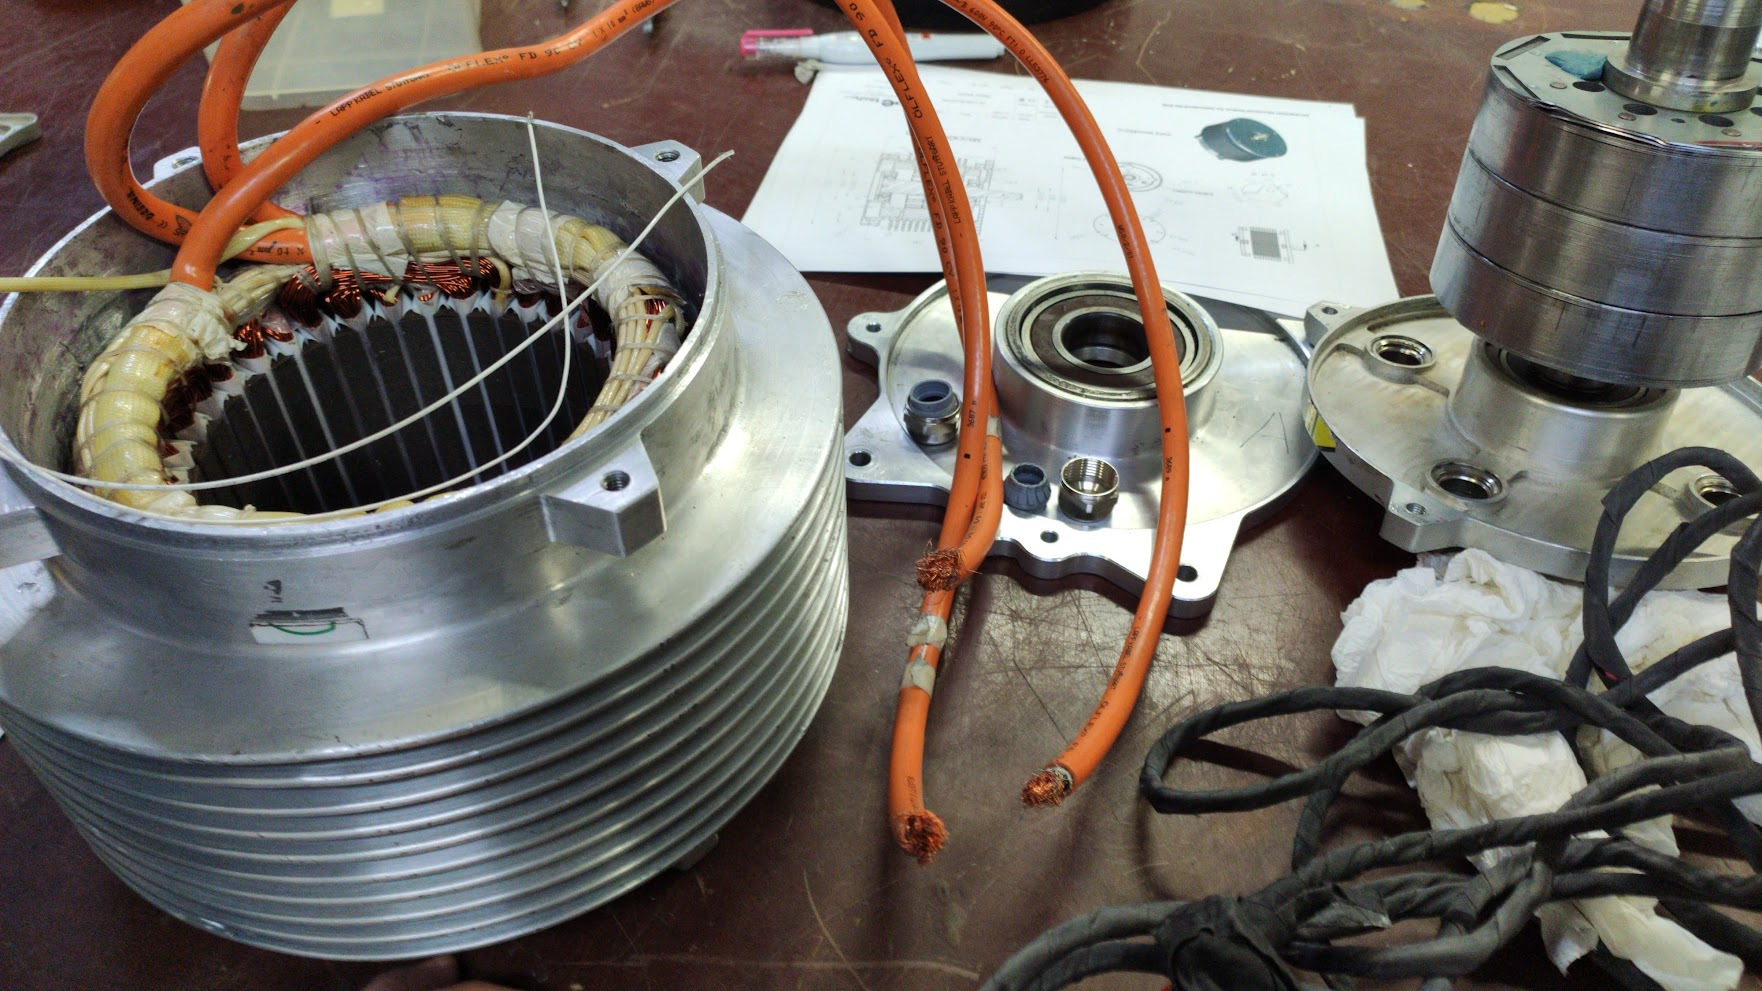
\includegraphics[width=0.7\linewidth]{fig/MVIMG_20220302_114007.jpg}
	\caption{Motor síncrono de imanes permanentes desmontado, de manera que se pueden ver los empilados del rotor y el estátor, los imanes y el bobinado.}
\end{figure}


Se trabajará con motores cuyos devanados estén conectados en configuración estrella, ya que se utiliza con mucha más frecuencia que la configuración delta. De todas maneras, es sencillo extender el modelo y el control a motores con conexión delta.


\begin{figure}[H]
	\centering
	\begin{circuitikz}
		% Draw three phases
		\draw (0,0) to [L, l=$L_s$, o-] ++(2,0) to [R, l=$R_s$] ++(2,0) to [sV, v=$e_a$] ++(2,0) -- ++(0,-2){};
		
		\draw (0,-2) to [L, l=$L_s$, o-] ++(2,0) to [R, l=$R_s$] ++(2,0) to [sV, v=$e_b$] ++(2,0) -- ++(0,2);
		
		\draw (0,-4) to [L, l=$L_s$, o-] ++(2,0) to [R, l=$R_s$] ++(2,0) to [sV, v=$e_c$] ++(2,0) -- ++(0,2);
		
		% Draw neutral point
		\draw (6,-2) node[circ]{} -- ++(0.5,0) node[circ]{} node[right]{$N$};
	\end{circuitikz}
	\caption{Circuito eléctrico equivalente de un PMSM trifásico en configuración estrella.}
\end{figure}

\subsection{Representación en el espacio vectorial}

Cuando el PMSM gira, las formas de onda de corriente y voltaje son aproximadamente senoidales. Se representan las formas de onda de la corriente en la figura \ref{3phaseVoltage}.

\begin{figure}[H]
    \centering
    \hspace*{-1.5cm}
    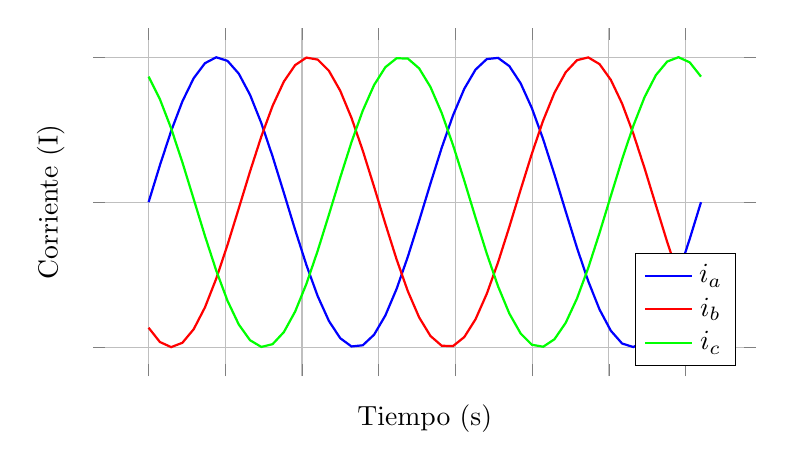
\begin{tikzpicture}
    \begin{axis}[
        width=10cm,
        height=6cm,
        xlabel={Tiempo (s)},
        ylabel={Corriente (I)},
        legend entries={$i_a$, $i_b$, $i_c$},
        grid=major,  
        legend pos=south east,
        samples=50,
        domain=0:2*360,
        axis line style={draw=none},  % Elimina el recuadro exterior
        xticklabels=\empty,  % Elimina las marcas en el eje x
        yticklabels=\empty,  % Elimina las marcas en el eje y
    ]
    \addplot[blue, thick, domain=0:2*360] {sin(x)};
    \addplot[red, thick, domain=0:2*360] {sin(x - 120)};
    \addplot[green, thick, domain=0:2*360] {sin(x - 240)};
    \end{axis}
    \end{tikzpicture}
    \caption{Sistema trifásico representado en el tiempo.}
    \label{3phaseVoltage}
\end{figure}

Todas las ecuaciones se pueden definir a partir de este modelo, pero se vuelve muy poco práctico para análisis más complejos. Se introduce una forma de representar estas formas de onda en el espacio tridimensional $\mathbb{R}^3$, en el que se escogen los ejes \((a, b, c)\). Lo que debería esperarse ver es una forma tridimensional en el espacio $\mathbb{R}^3$. Se comienza en \(t = 0\) y se dibuja un punto en las coordenadas \([i_a(0), i_b(0), i_c(0)]\). Luego, se continúa trazando puntos mientras se avanza a lo largo del eje del tiempo. La forma se puede expresar como curva paramétrica \([i_a(t), i_b(t), i_c(t)]\). Cuando se representa la forma resultante, puede sorprender, ya que es un círculo perfectamente plano. Cabe destacar que el orden de los ejes depende del contexto, y en este trabajo se toma el sistema de referencia mostrado en la figura \ref{spaceVectorGuapo}.


\begin{figure}[H]
    \centering
    \begin{subfigure}[b]{3cm}
        \centering
        \hspace*{-1.5cm}
        \begin{tikzpicture}
        \begin{axis}[
            %view={-45}{-35},
            view={-20}{-15},
            %view={54.74}{-15},
            axis lines=none,
            xmin=-1.5,
            xmax=1.5,
            ymin=-1.5,
            ymax=1.5,
            zmin=-1.5,
            zmax=1.5,
            no markers,
            axis equal,
            enlargelimits={upper=0.2},
            scale=1,
        ]
        \addplot3+[red, thick, no markers, samples=30, domain=-pi:pi, variable=\t]
            ({sin(deg(\t))}, {sin(deg(\t + 2*pi/3))}, {sin(deg(\t - 2*pi/3))});
       	
       % Ejes abc
       \draw[red, line width=1.5pt, -{Latex[length=1.5mm,width=1mm]}] (axis cs:0, 0, 0) -- (axis cs:0.5, 0, 0) node[pos=1.5]{$b$};
       \draw[red, line width=1.5pt, -{Latex[length=1.5mm,width=1mm]}] (axis cs:0, 0, 0) -- (axis cs:0, 0.5, 0) node[pos=1.5]{$a$};
       \draw[red, line width=1.5pt, -{Latex[length=1.5mm,width=1mm]}] (axis cs:0, 0, 0) -- (axis cs:0, 0, 0.5) node[pos=1.5]{$c$};
       
       \addplot3[draw=gray, no markers] coordinates {(-1.1, -1.1, -1.1) (-1.1, 1.1, -1.1)};
        \addplot3[draw=gray, no markers] coordinates {(-1.1, 1.1, -1.1) (1.1, 1.1, -1.1)};
        \addplot3[draw=gray, no markers] coordinates {(1.1, 1.1, -1.1) (1.1, -1.1, -1.1)};
        \addplot3[draw=gray, no markers] coordinates {(1.1, -1.1, -1.1) (-1.1, -1.1, -1.1)};
        \addplot3[draw=gray, no markers] coordinates {(-1.1, -1.1, 1.1) (-1.1, 1.1, 1.1)};
        \addplot3[draw=gray, no markers] coordinates {(-1.1, 1.1, 1.1) (1.1, 1.1, 1.1)};
        \addplot3[draw=gray, no markers] coordinates {(1.1, 1.1, 1.1) (1.1, -1.1, 1.1)};
        \addplot3[draw=gray, no markers] coordinates {(1.1, -1.1, 1.1) (-1.1, -1.1, 1.1)};
        \addplot3[draw=gray, no markers] coordinates {(-1.1, -1.1, -1.1) (-1.1, -1.1, 1.1)};
        \addplot3[draw=gray, no markers] coordinates {(-1.1, 1.1, -1.1) (-1.1, 1.1, 1.1)};
        \addplot3[draw=gray, no markers] coordinates {(1.1, 1.1, -1.1) (1.1, 1.1, 1.1)};
        \addplot3[draw=gray, no markers] coordinates {(1.1, -1.1, -1.1) (1.1, -1.1, 1.1)};
        \end{axis}
        \end{tikzpicture}
    \end{subfigure}
    \hfill
    \begin{subfigure}[b]{3cm}
        \centering
            \hspace*{-1.5cm}
            \begin{tikzpicture}
            \begin{axis}[
                view={-45}{-35},
                %view={-20}{-15},
                %view={54.74}{-15},
                axis lines=none,  % Elimina los ejes
                xmin=-.9,
                xmax=.9,
                ymin=-.9,
                ymax=.9,
                zmin=-.9,
                zmax=.9,
                no markers,
                axis equal,
                enlargelimits={upper=0.2},
                scale=1,
            ]
            \addplot3+[red, thick, no markers, samples=30, domain=-pi:pi, variable=\t]
                ({sin(deg(\t))}, {sin(deg(\t + 2*pi/3))}, {sin(deg(\t - 2*pi/3))});
           
           	% Ejes abc
           	\draw[red, line width=1.5pt, -{Latex[length=1.5mm,width=1mm]}] (axis cs:0, 0, 0) -- (axis cs:0.5, 0, 0) node[pos=1.5]{$b$};
           	\draw[red, line width=1.5pt, -{Latex[length=1.5mm,width=1mm]}] (axis cs:0, 0, 0) -- (axis cs:0, 0.5, 0) node[pos=1.5]{$a$};
           	\draw[red, line width=1.5pt, -{Latex[length=1.5mm,width=1mm]}] (axis cs:0, 0, 0) -- (axis cs:0, 0, 0.5) node[pos=1.5]{$c$};
           	
            \addplot3[draw=gray, no markers] coordinates {(-1.1, -1.1, -1.1) (-1.1, 1.1, -1.1)};
            \addplot3[draw=gray, no markers] coordinates {(-1.1, 1.1, -1.1) (1.1, 1.1, -1.1)};
            \addplot3[draw=gray, no markers] coordinates {(1.1, 1.1, -1.1) (1.1, -1.1, -1.1)};
            \addplot3[draw=gray, no markers] coordinates {(1.1, -1.1, -1.1) (-1.1, -1.1, -1.1)};
            \addplot3[draw=gray, no markers] coordinates {(-1.1, -1.1, 1.1) (-1.1, 1.1, 1.1)};
            \addplot3[draw=gray, no markers] coordinates {(-1.1, 1.1, 1.1) (1.1, 1.1, 1.1)};
            \addplot3[draw=gray, no markers] coordinates {(1.1, 1.1, 1.1) (1.1, -1.1, 1.1)};
            \addplot3[draw=gray, no markers] coordinates {(1.1, -1.1, 1.1) (-1.1, -1.1, 1.1)};
            \addplot3[draw=gray, no markers] coordinates {(-1.1, -1.1, -1.1) (-1.1, -1.1, 1.1)};
            \addplot3[draw=gray, no markers] coordinates {(-1.1, 1.1, -1.1) (-1.1, 1.1, 1.1)};
            \addplot3[draw=gray, no markers] coordinates {(1.1, 1.1, -1.1) (1.1, 1.1, 1.1)};
            \addplot3[draw=gray, no markers] coordinates {(1.1, -1.1, -1.1) (1.1, -1.1, 1.1)};
            \end{axis}
            \end{tikzpicture}
    \end{subfigure}
    \hfill
    \begin{subfigure}[b]{3cm}
        \centering
        \hspace*{-1.5cm}
        \begin{tikzpicture}
        \begin{axis}[
            %view={-45}{-35},
            %view={-20}{-15},
            view={54.7356103}{-15},
            axis lines=none,
            xmin=-1.5,
            xmax=1.5,
            ymin=-1.5,
            ymax=1.5,
            zmin=-1.5,
            zmax=1.5,
            no markers,
            axis equal,
            enlargelimits={upper=0.2},
            scale=1,
        ]
        \addplot3+[red, thick, no markers, samples=50, domain=-pi:pi, variable=\t]
            ({sin(deg(\t))}, {sin(deg(\t + 2*pi/3))}, {sin(deg(\t - 2*pi/3))});
        
        % Ejes abc
        \draw[red, line width=1.5pt, -{Latex[length=1.5mm,width=1mm]}] (axis cs:0, 0, 0) -- (axis cs:0.5, 0, 0) node[pos=1.5]{$b$};
        \draw[red, line width=1.5pt, -{Latex[length=1.5mm,width=1mm]}] (axis cs:0, 0, 0) -- (axis cs:0, 0.5, 0) node[pos=1.5]{$a$};
        \draw[red, line width=1.5pt, -{Latex[length=1.5mm,width=1mm]}] (axis cs:0, 0, 0) -- (axis cs:0, 0, 0.5) node[pos=1.5]{$c$};
        
         \addplot3[draw=gray, no markers] coordinates {(-1.1, -1.1, -1.1) (-1.1, 1.1, -1.1)};
        \addplot3[draw=gray, no markers] coordinates {(-1.1, 1.1, -1.1) (1.1, 1.1, -1.1)};
        \addplot3[draw=gray, no markers] coordinates {(1.1, 1.1, -1.1) (1.1, -1.1, -1.1)};
        \addplot3[draw=gray, no markers] coordinates {(1.1, -1.1, -1.1) (-1.1, -1.1, -1.1)};
        \addplot3[draw=gray, no markers] coordinates {(-1.1, -1.1, 1.1) (-1.1, 1.1, 1.1)};
        \addplot3[draw=gray, no markers] coordinates {(-1.1, 1.1, 1.1) (1.1, 1.1, 1.1)};
        \addplot3[draw=gray, no markers] coordinates {(1.1, 1.1, 1.1) (1.1, -1.1, 1.1)};
        \addplot3[draw=gray, no markers] coordinates {(1.1, -1.1, 1.1) (-1.1, -1.1, 1.1)};
        \addplot3[draw=gray, no markers] coordinates {(-1.1, -1.1, -1.1) (-1.1, -1.1, 1.1)};
        \addplot3[draw=gray, no markers] coordinates {(-1.1, 1.1, -1.1) (-1.1, 1.1, 1.1)};
        \addplot3[draw=gray, no markers] coordinates {(1.1, 1.1, -1.1) (1.1, 1.1, 1.1)};
        \addplot3[draw=gray, no markers] coordinates {(1.1, -1.1, -1.1) (1.1, -1.1, 1.1)};
        \end{axis}
        \end{tikzpicture}
    \end{subfigure}   
    \centering
    \caption{Sistema trifásico representado en el Espacio Vectorial.}
    \label{spaceVectorGuapo}
\end{figure}


Se puede observar que el sistema trifásico, cuando está equilibrado, se puede representar con solo dos variables, ya que la forma resultante es bidimensional. Se explorará cómo simplificar esto para facilitar el control del PMSM.

\subsection{Transformadas}

Se puede sospechar que lo que se necesita para representar el sistema trifásico con dos variables es un cambio de base. El enfoque general sería utilizar la transformada de Concordia. La transformada de Clarke es el caso particular para 3 dimensiones de la transformada de Concordia, que se utiliza para cualquier número de dimensiones.

Se pueden encontrar dos transformadas de Clarke: la transformada de Clarke ortonormal y la transformada de Clarke de amplitud constante o módulo invariante. Además, se pueden considerar el eje $\alpha$ avanzado 90º respecto al eje $\beta$, o viceversa. Para el análisis y control de una máquina eléctrica se suele utilizar la transformada de Clarke de amplitud constante con $\alpha$ avanzada.

\subsubsection{Transformada de Clarke ortonormal}

Esta transformada se utiliza cuando la potencia del sistema debe permanecer inalterada después de la transformación. Se aplican dos rotaciones al marco de referencia $abc$ y se crea el marco de referencia $\alpha\beta\gamma$. En este nuevo marco de referencia, la trayectoria del vector espacial está completamente contenida en el plano $\alpha\beta$ cuando el sistema está equilibrado, y el eje $\gamma$ se utiliza para explicar el componente homopolar del sistema (la suma de los tres componentes debe ser igual a 0 si el sistema está equilibrado, de lo contrario, aparece el componente homopolar).

\begin{figure}[H]
	\centering
	\hspace*{-1.5cm}
	\begin{tikzpicture}
		\begin{axis}[
			view={-45}{-35},
			%view={-20}{-15},
			%view={54.74}{-15},
			axis lines=none,  % Elimina los ejes
			xmin=-.9,
			xmax=.9,
			ymin=-.9,
			ymax=.9,
			zmin=-.9,
			zmax=.9,
			no markers,
			axis equal,
			enlargelimits={upper=0.2},
			scale=1,
			]
			\addplot3+[red, thick, no markers, samples=30, domain=-pi:pi, variable=\t]
			({sin(deg(\t))}, {sin(deg(\t + 2*pi/3))}, {sin(deg(\t - 2*pi/3))});
			
			% Ejes abc
			\draw[red, line width=1.5pt, -{Latex[length=1.5mm,width=1mm]}] (axis cs:0, 0, 0) -- (axis cs:0.5, 0, 0) node[pos=1.5]{$b$};
			\draw[red, line width=1.5pt, -{Latex[length=1.5mm,width=1mm]}] (axis cs:0, 0, 0) -- (axis cs:0, 0.5, 0) node[pos=1.5]{$a$};
			\draw[red, line width=1.5pt, -{Latex[length=1.5mm,width=1mm]}] (axis cs:0, 0, 0) -- (axis cs:0, 0, 0.5) node[pos=1.5]{$c$};
			
			% Ejes alpha-beta
			\draw[blue, line width=0.5pt, -{Latex[length=1.5mm,width=1mm]}] (axis cs:0, 0, 0) -- (axis cs:0, 0.7, 0) node[pos=1.5]{$\alpha$};
			\draw[blue, line width=0.5pt, -{Latex[length=1.5mm,width=1mm]}] (axis cs:0, 0, 0) -- (axis cs:1, 0.7, 0.3) node[pos=1.5]{$\beta$};

			\addplot3[draw=gray, no markers] coordinates {(-1.1, -1.1, -1.1) (-1.1, 1.1, -1.1)};
			\addplot3[draw=gray, no markers] coordinates {(-1.1, 1.1, -1.1) (1.1, 1.1, -1.1)};
			\addplot3[draw=gray, no markers] coordinates {(1.1, 1.1, -1.1) (1.1, -1.1, -1.1)};
			\addplot3[draw=gray, no markers] coordinates {(1.1, -1.1, -1.1) (-1.1, -1.1, -1.1)};
			\addplot3[draw=gray, no markers] coordinates {(-1.1, -1.1, 1.1) (-1.1, 1.1, 1.1)};
			\addplot3[draw=gray, no markers] coordinates {(-1.1, 1.1, 1.1) (1.1, 1.1, 1.1)};
			\addplot3[draw=gray, no markers] coordinates {(1.1, 1.1, 1.1) (1.1, -1.1, 1.1)};
			\addplot3[draw=gray, no markers] coordinates {(1.1, -1.1, 1.1) (-1.1, -1.1, 1.1)};
			\addplot3[draw=gray, no markers] coordinates {(-1.1, -1.1, -1.1) (-1.1, -1.1, 1.1)};
			\addplot3[draw=gray, no markers] coordinates {(-1.1, 1.1, -1.1) (-1.1, 1.1, 1.1)};
			\addplot3[draw=gray, no markers] coordinates {(1.1, 1.1, -1.1) (1.1, 1.1, 1.1)};
			\addplot3[draw=gray, no markers] coordinates {(1.1, -1.1, -1.1) (1.1, -1.1, 1.1)};
		\end{axis}
	\end{tikzpicture}
	\centering
	\caption{Sistema trifásico representado en el Espacio Vectorial con la transformada de Clarke ortonormal superpuesta.}
	\end{figure}

Representar esta transformada en un eje temporal refleja de forma más intuitiva el resultado.
\begin{figure}[H]
	\centering
	\hspace*{-1.5cm}
	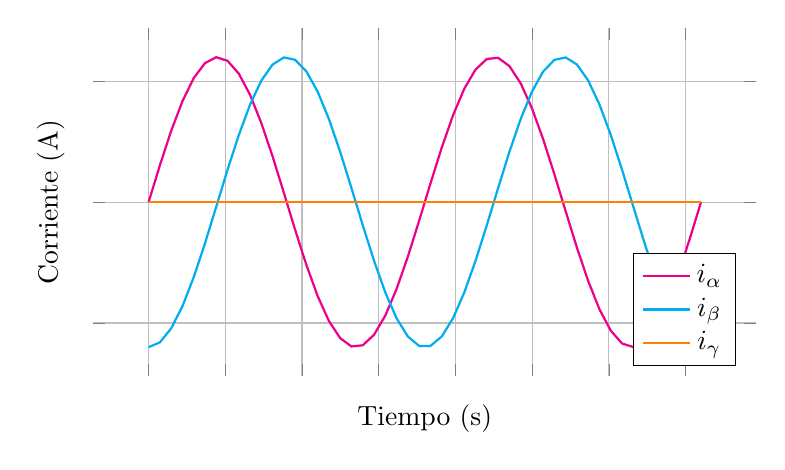
\begin{tikzpicture}
		\begin{axis}[
			width=10cm,
			height=6cm,
			xlabel={Tiempo (s)},
			ylabel={Corriente (A)},
			legend entries={$i_{\alpha}$, $i_{\beta}$, $i_{\gamma}$},
			grid=major,  
			legend pos=south east,
			samples=50,
			domain=0:2*360,
			axis line style={draw=none},  % Elimina el recuadro exterior
			xticklabels=\empty,  % Elimina las marcas en el eje x
			yticklabels=\empty,  % Elimina las marcas en el eje y
			]
		
			\addplot[magenta, thick, domain=0:2*360] {1.2*sin(x)};
			\addplot[cyan, thick, domain=0:2*360] {1.2*sin(x - 90)};
			\addplot[orange, thick, domain=0:2*360] {0};
		\end{axis}
	\end{tikzpicture}
	\caption{Transformada de Clarke ortonormal representada en el tiempo.}
\end{figure}



No se derivará la transformada aquí, aunque es necesario comprender lo que hace y conocer la matriz de transformación.

Lo que hace la transformada es colocar dos de los ejes del sistema de referencia en el plano formado por el círculo generado por el vector espacial. El eje restante es perpendicular a ese plano y representa el componente homopolar.

La forma matricial de la transformada es

\begin{equation}
    \begin{bmatrix}
        \alpha \\
        \beta \\
        \gamma
    \end{bmatrix}
    =
    \sqrt{\frac{2}{3}}
    \begin{bmatrix}
        1 & -\frac{1}{2} & -\frac{1}{2} \\
        0 & \frac{\sqrt{3}}{2} & -\frac{\sqrt{3}}{2} \\
        \frac{1}{\sqrt{2}} & \frac{1}{\sqrt{2}} & \frac{1}{\sqrt{2}}
    \end{bmatrix}
    \begin{bmatrix}
        a \\
        b \\
        c
    \end{bmatrix} \text{ .}
\end{equation}

La forma matricial de la transformada inversa es

\begin{equation}
    \begin{bmatrix}
        a \\
        b \\
        c
    \end{bmatrix}
    =
    \sqrt{\frac{2}{3}}
    \begin{bmatrix}
        1 & 0 & \frac{1}{\sqrt{2}} \\
        -\frac{1}{2} & \frac{\sqrt{3}}{2} & \frac{1}{\sqrt{2}} \\
        -\frac{1}{2} & -\frac{\sqrt{3}}{2} & \frac{1}{\sqrt{2}}
    \end{bmatrix}
    \begin{bmatrix}
        \alpha \\
        \beta \\
        \gamma
    \end{bmatrix} \text{ .}
\end{equation}

Esta transformada tiene la particularidad de mantener constante la potencia del sistema, de modo que se cumple que

\begin{equation}
p(t) = p_{abc} = p_{\alpha\beta\gamma, \text{ortonormal}} = v_a \cdot i_a + v_b \cdot i_b + v_c \cdot i_c = v_\alpha \cdot i_\alpha + v_\beta \cdot i_\beta + v_\gamma \cdot i_\gamma \text{ .}
\end{equation}

\subsubsection{Transformada de Clarke de amplitud constante}

Mantener constante la potencia a lo largo de las transformadas puede ser útil en algunos contextos, pero lo que se suele implementar es una variante de la transformada de Clarke que mantiene constante la amplitud de la magnitud.

La transformada no es ortonormal, ya que ajusta las magnitudes para que el módulo de las variables sea el adecuado, pero la rotación se mantiene igual.

\begin{figure}[H]
	\centering
	\hspace*{-1.5cm}
	\begin{tikzpicture}
		\begin{axis}[
			view={-45}{-35},
			%view={-20}{-15},
			%view={54.74}{-15},
			axis lines=none,  % Elimina los ejes
			xmin=-.9,
			xmax=.9,
			ymin=-.9,
			ymax=.9,
			zmin=-.9,
			zmax=.9,
			no markers,
			axis equal,
			enlargelimits={upper=0.2},
			scale=1,
			]
			\addplot3+[red, thick, no markers, samples=30, domain=-pi:pi, variable=\t]
			({sin(deg(\t))}, {sin(deg(\t + 2*pi/3))}, {sin(deg(\t - 2*pi/3))});
			
			% Ejes abc
			\draw[red, line width=1.5pt, -{Latex[length=1.5mm,width=1mm]}] (axis cs:0, 0, 0) -- (axis cs:0.5, 0, 0) node[pos=1.5]{$b$};
			\draw[red, line width=1.5pt, -{Latex[length=1.5mm,width=1mm]}] (axis cs:0, 0, 0) -- (axis cs:0, 0.5, 0) node[pos=1.5]{$a$};
			\draw[red, line width=1.5pt, -{Latex[length=1.5mm,width=1mm]}] (axis cs:0, 0, 0) -- (axis cs:0, 0, 0.5) node[pos=1.5]{$c$};
			
			% Ejes alpha-beta
			\draw[blue, line width=0.5pt, -{Latex[length=1.5mm,width=1mm]}] (axis cs:0, 0, 0) -- (axis cs:0, 0.5, 0) node[pos=1.5]{$\alpha'$};
			\draw[blue, line width=0.5pt, -{Latex[length=1.5mm,width=1mm]}] (axis cs:0, 0, 0) -- (axis cs:0.8, 0.6, 0.25) node[pos=1.5]{$\beta'$};
			
			\addplot3[draw=gray, no markers] coordinates {(-1.1, -1.1, -1.1) (-1.1, 1.1, -1.1)};
			\addplot3[draw=gray, no markers] coordinates {(-1.1, 1.1, -1.1) (1.1, 1.1, -1.1)};
			\addplot3[draw=gray, no markers] coordinates {(1.1, 1.1, -1.1) (1.1, -1.1, -1.1)};
			\addplot3[draw=gray, no markers] coordinates {(1.1, -1.1, -1.1) (-1.1, -1.1, -1.1)};
			\addplot3[draw=gray, no markers] coordinates {(-1.1, -1.1, 1.1) (-1.1, 1.1, 1.1)};
			\addplot3[draw=gray, no markers] coordinates {(-1.1, 1.1, 1.1) (1.1, 1.1, 1.1)};
			\addplot3[draw=gray, no markers] coordinates {(1.1, 1.1, 1.1) (1.1, -1.1, 1.1)};
			\addplot3[draw=gray, no markers] coordinates {(1.1, -1.1, 1.1) (-1.1, -1.1, 1.1)};
			\addplot3[draw=gray, no markers] coordinates {(-1.1, -1.1, -1.1) (-1.1, -1.1, 1.1)};
			\addplot3[draw=gray, no markers] coordinates {(-1.1, 1.1, -1.1) (-1.1, 1.1, 1.1)};
			\addplot3[draw=gray, no markers] coordinates {(1.1, 1.1, -1.1) (1.1, 1.1, 1.1)};
			\addplot3[draw=gray, no markers] coordinates {(1.1, -1.1, -1.1) (1.1, -1.1, 1.1)};
		\end{axis}
	\end{tikzpicture}
	\centering
	\caption{Sistema trifásico representado en el Espacio Vectorial con la transformada de Clarke de amplitud constante superpuesta.}
\end{figure}

\begin{figure}[H]
	\centering
	\hspace*{-1.5cm}
	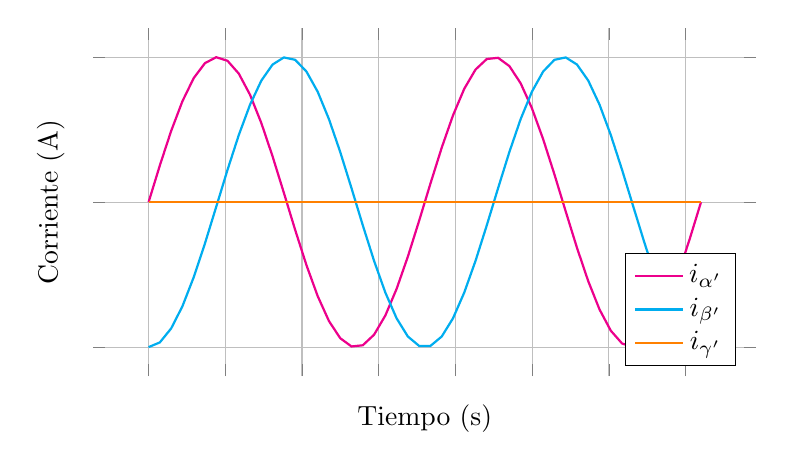
\begin{tikzpicture}
		\begin{axis}[
			width=10cm,
			height=6cm,
			xlabel={Tiempo (s)},
			ylabel={Corriente (A)},
			legend entries={$i_{\alpha'}$, $i_{\beta'}$, $i_{\gamma'}$},
			grid=major,  
			legend pos=south east,
			samples=50,
			domain=0:2*360,
			axis line style={draw=none},  % Elimina el recuadro exterior
			xticklabels=\empty,  % Elimina las marcas en el eje x
			yticklabels=\empty,  % Elimina las marcas en el eje y
			]
			
			\addplot[magenta, thick, domain=0:2*360] {sin(x)};
			\addplot[cyan, thick, domain=0:2*360] {sin(x - 90)};
			\addplot[orange, thick, domain=0:2*360] {0};
		\end{axis}
	\end{tikzpicture}
	\caption{Transformada de Clarke de amplitud constante representada en el tiempo.}
\end{figure}

De esta manera, la forma matricial de la transformada de amplitud constante es
\begin{equation}
    \begin{bmatrix}
        \alpha' \\
        \beta' \\
        \gamma'
    \end{bmatrix}
    =
    \frac{2}{3}
    \begin{bmatrix}
        1 & -\frac{1}{2} & -\frac{1}{2} \\
        0 & \frac{\sqrt{3}}{2} & -\frac{\sqrt{3}}{2} \\
        \frac{1}{2} & \frac{1}{2} & \frac{1}{2}
    \end{bmatrix}
    \begin{bmatrix}
        a \\
        b \\
        c
    \end{bmatrix} \text{ .}
\end{equation}

Y la de la transformada inversa es 

\begin{equation}
    \begin{bmatrix}
        a \\
        b \\
        c
    \end{bmatrix}
    =
    \begin{bmatrix}
        1 & 0 & 1 \\
        -\frac{1}{2} & \frac{\sqrt{3}}{2} & 1 \\
        -\frac{1}{2} & -\frac{\sqrt{3}}{2} & 1
    \end{bmatrix}
    \begin{bmatrix}
        \alpha' \\
        \beta' \\
        \gamma'
    \end{bmatrix} \text{ .}
\end{equation}

Se puede derivar que

\begin{equation}
p_{abc} = \frac{3}{2} \cdot (v_{\alpha'} \cdot i_{\alpha'} + v_{\beta'} \cdot i_{\beta'} + v_{\gamma'} \cdot i_{\gamma'}) \text{ .}
\end{equation}


\subsubsection{Transformada de Park}

Después de aplicar la transformada de Clarke, todavía quedan dos variables sinusoidales (\(\alpha\beta\) si se considera \(\gamma = 0\)), lo que dificulta el análisis para que el control sea sencillo. Por lo tanto, se aplica otra transformada para convertir estas cantidades sinusoidales en constantes.

Ahora, considerando que el vector espacial gira a una velocidad de \(\omega = 2\pi f\), si se aplica continuamente una rotación alrededor del eje \(\gamma\) con un ángulo \(\theta = \omega  t\), se puede representar el vector espacial como una composición de dos variables continuas (en lugar de sinusoides). Además, si se sincroniza esta rotación con el ángulo del vector espacial (el eje \(d\) apuntando al vector espacial), se obtiene una variable continua (\(q\)) y una segunda variable de valor nulo (\(d\)).

\begin{figure}[H]
  	\centering
  \hspace*{-1.5cm}
  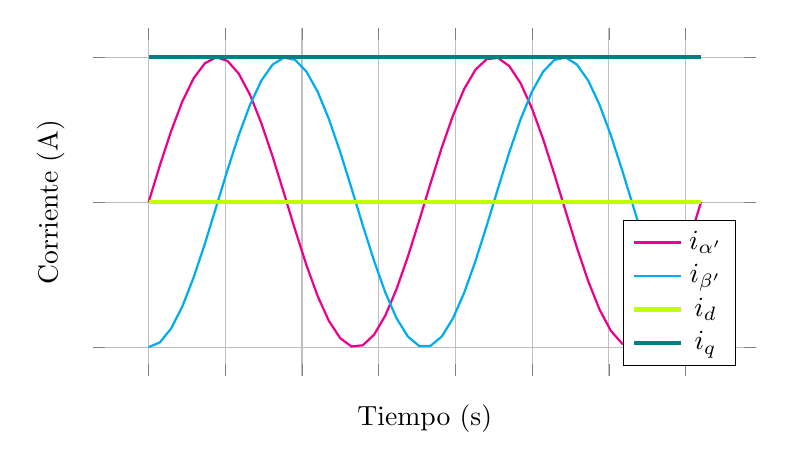
\begin{tikzpicture}
  	\begin{axis}[
  		width=10cm,
  		height=6cm,
  		xlabel={Tiempo (s)},
  		ylabel={Corriente (A)},
  		legend entries={$i_{\alpha'}$, $i_{\beta'}$, $i_d$, $i_q$},
  		grid=major,  
  		legend pos=south east,
  		samples=50,
  		domain=0:2*360,
  		axis line style={draw=none},  % Elimina el recuadro exterior
  		xticklabels=\empty,  % Elimina las marcas en el eje x
  		yticklabels=\empty,  % Elimina las marcas en el eje y
  		]
  		
  		\addplot[magenta, thick, domain=0:2*360] {sin(x)};
  		\addplot[cyan, thick, domain=0:2*360] {sin(x - 90)};
  		
  		\addplot[lime, ultra thick, domain=0:2*360] {0};
  		\addplot[teal, ultra thick, domain=0:2*360] {1};
  		
  		
  	\end{axis}
  \end{tikzpicture}
  \caption{Transformada de Park representada en el tiempo junto a la transformada de Clarke de amplitud constante.}
\end{figure}

Se puede ver que la transformada es simplemente una rotación a lo largo de uno de los ejes de la base, de manera que 

\begin{equation}
    \begin{bmatrix}
        d \\
        q \\
        0
    \end{bmatrix}
    =
    \begin{bmatrix}
        \cos(\theta) & \sin(\theta) & 0 \\
        -\sin(\theta) & \cos(\theta) & 0 \\
        0 & 0 & 1
    \end{bmatrix}
    \begin{bmatrix}
        \alpha \\
        \beta \\
        \gamma
    \end{bmatrix} \text{ .}
\end{equation}

\subsection{Marco de referencia rotatorio}

En esta sección, se convertirá el modelo trifásico inicial del PMSM en un modelo continuo en el marco de referencia $d - q$. Antes, se omitieron las ecuaciones del modelo trifásico, que se pueden encontrar en \cite{MathworksPMSM}, pero utilizando estas y aplicando las transformadas de Clarke y Park, se obtienen las ecuaciones que se derivarán en esta sección.

El enfoque general es utilizar la transformada de amplitud constante, por lo que para las tensiones y corrientes del estátor se utiliza

\begin{equation}
	\begin{bmatrix}
		v_d \\
		v_q \\
		v_0
	\end{bmatrix}
	=
	\begin{bmatrix}
		\cos(\theta) & \sin(\theta) & 0  \\
		-\sin(\theta) & \cos(\theta) & 0  \\
		0 & 0 & 1
	\end{bmatrix}
	\frac{2}{3}
	\begin{bmatrix}
		1 & -\frac{1}{2} & -\frac{1}{2} \\
		0 & \frac{\sqrt{3}}{2} & -\frac{\sqrt{3}}{2} \\
		\frac{1}{2} & \frac{1}{2} & \frac{1}{2}
	\end{bmatrix}
	\begin{bmatrix}
		v_a \\
		v_b \\
		v_c
	\end{bmatrix}
\end{equation}

y

\begin{equation}
	\begin{bmatrix}
		i_d \\
		i_q \\
		i_0
	\end{bmatrix}
	=
	\begin{bmatrix}
		\cos(\theta) & \sin(\theta) & 0  \\
		-\sin(\theta) & \cos(\theta) & 0  \\
		0 & 0 & 1
	\end{bmatrix}
	\frac{2}{3}
	\begin{bmatrix}
		1 & -\frac{1}{2} & -\frac{1}{2} \\
		0 & \frac{\sqrt{3}}{2} & -\frac{\sqrt{3}}{2} \\
		\frac{1}{2} & \frac{1}{2} & \frac{1}{2}
	\end{bmatrix}
	\begin{bmatrix}
		i_a \\
		i_b \\
		i_c
	\end{bmatrix} \text{.}
\end{equation}

El modelo de circuito equivalente se divide en los circuitos del eje $d$ y el eje $q$.

\begin{figure}[H]
	\centering
	\begin{minipage}{0.45\textwidth}
		\centering
		\begin{circuitikz}[american voltages]
			% d-axis circuit
			\draw (0,0) to [L, l=$L_d$, o-] ++(2,0) to [R, l=$R_s$] ++(2,0) to [V, v^=$\omega_e\cdot L_q\cdot i_q$, invert] ++(2,0) -- ++(0,-2){};
			% Parallel line
			\draw (0,-2) node[circ, fill=none]{} -- ++(6,0);
			% Current label
			\draw (4,-2) to [open, i_=$i_d$] (2,-2);
			% Voltage labels
			\draw (0,0) to [open, v^=$v_d$] (0,-2);
		\end{circuitikz}
	\end{minipage}
	\hspace{0.05\textwidth}
	\begin{minipage}{0.45\textwidth}
		\centering
		\begin{circuitikz}[american voltages]
			% q-axis circuit
			\draw (0,0) to [L, l=$L_q$, o-] ++(2,0) to [R, l=$R_s$] ++(2,0) to [V, v^=$\omega_e\cdot L_d\cdot i_d$] ++(2,0) to [V, v^=$\omega_e\cdot\lambda_m$] ++(0,-2){};
			% Parallel line
			\draw (0,-2) node[circ, fill=none]{} -- ++(6,0);
			% Current label
			\draw (4,-2) to [open, i_=$i_q$] (2,-2);
			% Voltage labels
			\draw (0,0) to [open, v^=$v_q$] (0,-2);
		\end{circuitikz}
	\end{minipage}
	\caption{Circuitos eléctricos equivalentes del modelo $d-q$ de un PMSM.}
\end{figure}

Se puede observar que

\begin{equation}
v_d = v_{R_s} - \omega_e \cdot L_q \cdot i_q + v_{L_d}
\end{equation}

\begin{equation}
v_d = R_s\cdot i_d - \omega_e \cdot L_q \cdot i_q + L_d\cdot\frac{d i_d}{d t}
\end{equation}

y

\begin{equation}
v_q = v_{R_s} - \omega_e \cdot L_d \cdot i_d + \omega_e \cdot \lambda_m + v_{L_q}
\end{equation}

\begin{equation}
v_q = R_s\cdot i_q - \omega_e \cdot L_d \cdot i_d + \omega_e \cdot \lambda_m + L_q\cdot\frac{d i_q}{d t}  \text{ .}
\end{equation}

En estado estacionario, es decir, sin cambios muy bruscos de la corriente, el término diferencial puede ser eliminado, de manera que

\begin{equation}
	v_d = R_s\cdot i_d - \omega_e \cdot L_q \cdot i_q
	\label{eq_vd}
\end{equation}
\begin{equation}
	v_q = R_s\cdot i_q - \omega_e \cdot L_d \cdot i_q + \omega_e \cdot \lambda_m \text{ ,}
	\label{eq_vq}
\end{equation}


donde
\begin{itemize}
    \item \(v_d\) y \(v_q\) son las tensiones en los ejes d y q respectivamente.
    \item \(i_d\) y \(i_q\) son las corrientes en los ejes d y q respectivamente.
    \item \(L_d\) y \(L_q\) son las inductancias en los ejes d y q respectivamente.
    \item \(\omega_e\) es la velocidad eléctrica, que es la velocidad mecánica multiplicada por el número de pares de polos del PMSM (\(\omega_e = \omega_m \cdot pp = \omega_m \cdot \frac{n}{2}\)).
    \item \(\lambda_m\) es el flujo magnético generado por los imanes permanentes. La magnitud del flujo magnético generado afecta directamente la magnitud de la tensión inducida en las fases del estátor. Este parámetro se puede transformar fácilmente en \(k_E\), que es la relación entre la velocidad mecánica del rotor y la tensión generada en las 3 fases.
\end{itemize}


Hay PMSM cuyos imanes están montados dentro del rotor (IPM) y otros cuyos imanes están en la superficie del rotor (SPM). Esta diferenciación juega un papel importante en el desarrollo del modelo y el control, porque en los SPM se cumple \(L_d = L_q\), a menudo escrito solo como \(L\). Además, si se trata de un IPM, la orientación de los imanes puede cambiar las trayectorias del control, de manera que si son imanes tangenciales se da \(L_d > L_q\) y si son imanes radiales \(L_d < L_q\). Se desarrollarán las ecuaciones para motores IPM con imanes radiales, pero se ha de tener en cuenta que se pueden realizar muchas simplificaciones si el motor es un SPM. Una situación que se dará es que algunas ecuaciones tienen alguna forma de \(L_d - L_q\) como denominador, lo cual es bastante problemático si se está tratando de implementar la ecuación directamente. Por ese motivo, es mejor diferenciar el tipo de motor antes de implementar las ecuaciones. Una solución válida es tener en cuenta la anisotropía magnética que suelen presentar la mayoría de SPMs, con lo que \(L_d < L_q\) y se pueden aplicar las ecuaciones del IPM a costa de potencia de cálculo, de ejecutarse el control en tiempo real.

\begin{figure}[H]
	\centering
	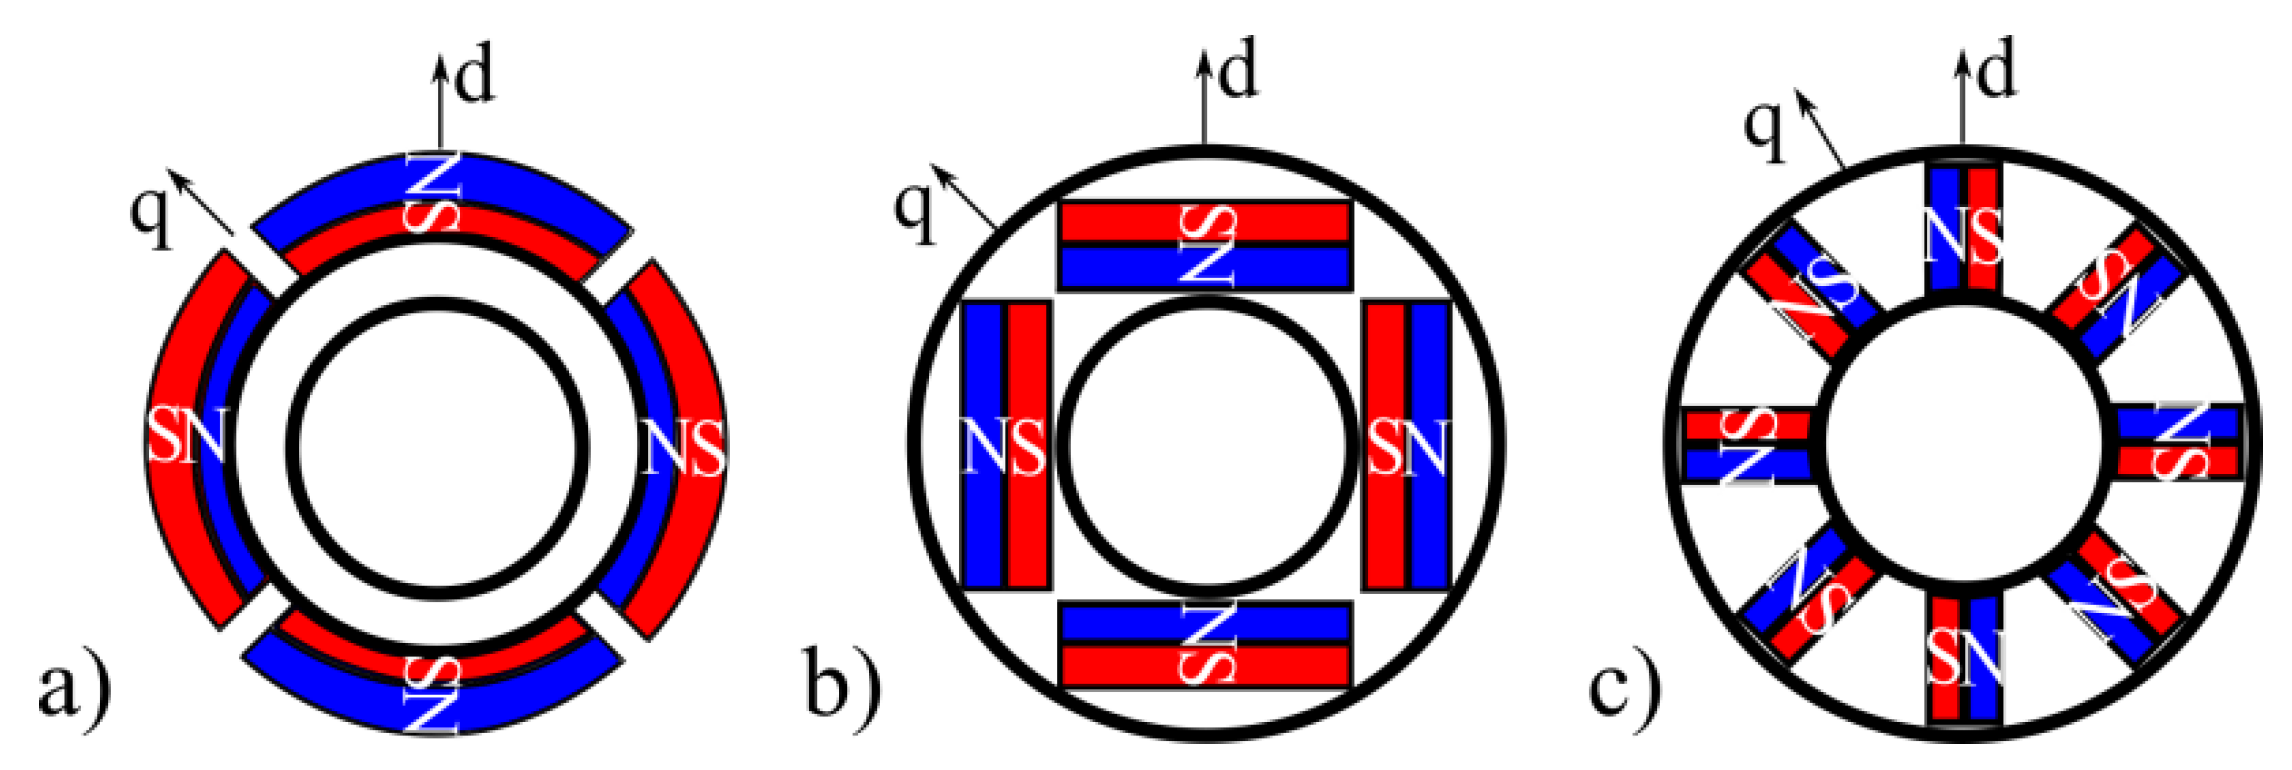
\includegraphics[width=0.7\linewidth]{fig/motor-types}
	\caption{Tipos de PMSMs según la disposición de los imanes. a) SPM, b) IPM radial, c) IPM tangencial. \cite{Sieklucki2022}}
\end{figure}


La potencia eléctrica se define como

\begin{equation}
p_e = \frac{3}{2}\cdot(v_d i_d + v_q i_q) \text{ .}
\end{equation}

Si se supone que la máquina es perfectamente eficiente, se puede decir que la potencia mecánica es igual a la potencia eléctrica, \(p_e = p_m\). Sabiendo que \(p_m = \omega_m T_{\text{em}}\), donde \(T_{\text{em}}\) es el par electromagnético producido, se puede derivar que

\begin{equation}
T_{\text{em}} = \frac{3}{2\cdot \omega_m}\cdot(v_d i_d + v_q i_q) = \frac{3}{2\cdot \omega_e}\frac{n}{2}\cdot(v_d i_d + v_q i_q)
\end{equation}

\begin{equation}
 \therefore T_{\text{em}} = \frac{3}{2}\frac{n}{2}\cdot((L_d - L_q) i_q i_d + \lambda_m i_q) \text{ .}
\label{eq_tq_dq} 
\end{equation}

También se puede establecer un límite de voltaje, porque el PMSM generalmente se controla con un inversor de fuente de voltaje (VSI) modulado por SVPWM y la tensión de salida $V_s$ está limitada a \(\frac{V_{\text{DC}}}{\sqrt{3}}\). En esta ecuación, no se considera la caída de tensión por la resistencia del estátor \(R_s\), ya que haría que las ecuaciones fueran muy densas y el efecto de esta caída de voltaje es despreciable a altas velocidades. Por ello,

\begin{equation}
v_s = \sqrt{v_d^2 + v_q^2} \leq \frac{V_{\text{DC}}}{\sqrt{3}}
\end{equation}
\begin{equation}
	 \therefore \sqrt{\left(R_s\cdot i_d - \omega_e \cdot L_q \cdot i_q\right)^2 + \left(R_s\cdot i_q - \omega_e \cdot L_d \cdot i_q + \omega_e \cdot \lambda_m\right)^2} \leq \frac{V_{\text{DC}}}{\sqrt{3}} \text{ .}
\end{equation}

Despreciando los términos con \(R_s\),
\begin{equation}
	\sqrt{\left(- \omega_e \cdot L_q \cdot i_q\right)^2 + \left(- \omega_e \cdot L_d \cdot i_q + \omega_e \cdot \lambda_m\right)^2} \leq \frac{V_{\text{DC}}}{\sqrt{3}} \text{ .}
\end{equation}
 
Y reordenando,
\begin{equation}
	\left(\frac{\frac{V_{\text{DC}}}{\sqrt{3}}}{\omega_e}\right)^2 \geq \left(\lambda_m+L_d\cdot i_d\right)^2+(L_q\cdot i_q)^2 \text{ .}
	\label{eq_vle_dq}
\end{equation}

\subsection{Curvas características del PMSM}

Las ecuaciones del PMSM son muy útiles cuando se diseña el control y la implementación real, pero antes de eso, es muy recomendable verlas en un gráfico para comprender mejor algunas de las intuiciones detrás de ellas.

\subsubsection{Curva de par-velocidad y potencia-velocidad}

Las primeras curvas estudiadas son las de par-velocidad y potencia-velocidad. Definen la intención de diseño del PMSM, ilustrando el rendimiento deseado. El objetivo al diseñar el control es tratar de igualar o incluso superar estas curvas.


\begin{figure}[H]
    \centering
    \hspace*{-1.5cm}
    \begin{tikzpicture}
    \begin{axis}[
        axis lines=middle,
        width=10cm,
        height=8cm,
        x label style={at={(axis description cs:-0.1,0.5)},anchor=north},
        y label style={at={(axis description cs:0.5,-0.1)},rotate=90,anchor=south},
        xlabel={$\omega_\text{m}$},
        ylabel={$T_{\text{em}}$},
        ytick={-26, 26},
        xtick={-2000,-1000,1000,2000},
        yticklabels={$-T_{\text{em,máx}}$, $T_{\text{em,máx}}$},
        xticklabels={$-\omega_{\text{m,máx}}$, $-\omega_{\text{m,nom}}$, $\omega_{\text{m,nom}}$,$\omega_{\text{m,máx}}$},
        grid=none,  
        ymin=-40,
        ymax=40,
        samples=15,
        domain=-2500:2500,
        nodes near coords align={south east},
        y tick label style={yshift={sign(\tick)*10}},
        ylabel style={rotate=-90},
        %no marks
        % axis line style={draw=none},  % Elimina el recuadro exterior
    ]
    \addplot[blue, thick, domain=-1000:1000] {26};
    \addplot[blue, thick, domain=-1000:1000] {-26};
    \addplot[blue, thick, domain=1000:2500] {26000/x};
    \addplot[blue, thick, domain=-2500:-1000] {-26000/x};
    \addplot[white, line width=1mm, domain=2000:2500] {26000/x};
    \addplot[white, line width=1mm, domain=-2500:-2000] {-26000/x};
    \addplot[blue, thick, domain=1000:2500] {-26000/x};
    \addplot[blue, thick, domain=-2500:-1000] {26000/x};
    \addplot[white, line width=1mm, domain=2000:2500] {-26000/x};
    \addplot[white, line width=1mm, domain=-2500:-2000] {26000/x};
    \end{axis}
    \end{tikzpicture}
    \caption{Curva de par-velocidad del PMSM.}
\end{figure}


La curva es una función por tramos, que toma \(T_{\text{em,máx}}\), \(\omega_{\text{m,máx}}\) y \(P_{\text{m,máx}}\) como sus parámetros.

La curva es constante desde \(\omega_\text{m} = 0\) hasta \(\omega_\text{m} = \omega_{\text{m,nom}} = \frac{P_{\text{m,máx}}}{T_{\text{em,máx}}}\), donde su valor es \(T_{\text{em,máx}}\). Esta porción es lo que se conoce como la zona de par constante. Desde \(\omega_\text{m} = \omega_{\text{m,nom}}\) hasta \(\omega_\text{m} = \omega_{\text{m,máx}}\), \(T_{\text{em}}\) se define como \(T_{\text{em}} = \frac{P_{\text{m,máx}}}{\omega_\text{m}}\), lo que da una curva de tipo \(y=\frac{a}{x}\). Esto se llama la zona de potencia constante.

\[
T_{\text{em}} = 
\begin{cases}
  T_{\text{em,máx}} & -\omega_{\text{m,nom}} < \omega_\text{m} < \omega_{\text{m,nom}} \\
  -T_{\text{em,máx}} & -\omega_{\text{m,nom}} < \omega_\text{m} < \omega_{\text{m,nom}} \\
  \frac{P_{\text{m,máx}}}{\omega_\text{m}} & \omega_{\text{m,nom}}\leq \omega_\text{m}\leq \omega_{\text{m,máx}} (T_{\text{em,máx}}),-\omega_{\text{m,máx}}\leq \omega_\text{m}\leq -\omega_{\text{m,nom}} (-T_{\text{em,máx}})\\
  -\frac{P_{\text{m,máx}}}{\omega_\text{m}} & \omega_{\text{m,nom}}\leq \omega_\text{m}\leq \omega_{\text{m,máx}} (-T_{\text{em,máx}}),-\omega_{\text{m,máx}}\leq \omega_\text{m}\leq -\omega_{\text{m,nom}} (T_{\text{em,máx}})
\end{cases}
\]

Además \(P_\text{m}\) aumentará linealmente con \(\omega_\text{m}\) hasta \(\omega_{\text{m,nom}}\), ya que \(P_\text{m} = T_{\text{em}} \cdot \omega_\text{m}\). Desde \(\omega_{\text{m,nom}}\) hasta \(\omega_{\text{m,máx}}\), \(P_\text{m}\) es una recta de valor \(P_{\text{m,máx}}\).

\begin{figure}[H]
	\centering
	\hspace*{-1.5cm}
	\begin{tikzpicture}
		\begin{axis}[
			axis lines=middle,
			width=10cm,
			height=8cm,
			x label style={at={(axis description cs:-0.1,0.5)},anchor=north},
			y label style={at={(axis description cs:0.5,-0.1)},rotate=90,anchor=south},
			xlabel={$\omega_\text{m}$},
			ylabel={$P_{\text{m}}$},
			ytick={-26, 26},
			xtick={-2000,-1000,1000,2000},
			yticklabels={$-P_{\text{m,máx}}$, $P_{\text{m,máx}}$},
			xticklabels={$-\omega_{\text{m,máx}}$, $-\omega_{\text{m,nom}}$, $\omega_{\text{m,nom}}$,$\omega_{\text{m,máx}}$},
			grid=none,  
			ymin=-40,
			ymax=40,
			samples=15,
			domain=-2500:2500,
			nodes near coords align={south east},
			y tick label style={yshift={sign(\tick)*10}},
			ylabel style={rotate=-90},
			%no marks
			% axis line style={draw=none},  % Elimina el recuadro exterior
			]
			\addplot[blue, thick, domain=-1000:1000] {x*26/1000};
			\addplot[blue, thick, domain=-1000:1000] {-x*26/1000};
			\addplot[blue, thick, domain=1000:2500] {26};
			\addplot[blue, thick, domain=-2500:-1000] {-26};
			\addplot[white, line width=1mm, domain=2000:2500] {26};
			\addplot[white, line width=1mm, domain=-2500:-2000] {-26};
			\addplot[blue, thick, domain=1000:2500] {-26};
			\addplot[blue, thick, domain=-2500:-1000] {26};
			\addplot[white, line width=1mm, domain=2000:2500] {-26};
			\addplot[white, line width=1mm, domain=-2500:-2000] {26};
		\end{axis}
	\end{tikzpicture}
	\caption{Curva de potencia-velocidad del PMSM.}
\end{figure}


\subsubsection{CLC (Círculo de Límite de Corriente)}

Es obvio que la corriente eléctrica suministrada al PMSM debe estar limitada. Por lo general, el fabricante del motor establecerá la corriente alterna máxima, lo cual se traduce en un límite para \(i_d\) y \(i_q\).

A continuación, se presenta un gráfico muy útil para conocer los límites del motor. Se establecen los ejes como $i_d$ e $i_q$. Por ejemplo, si un motor está funcionando con $i_d = -1 \text{ A}$ e $i_q = 5 \text{ A}$, se dibuja un punto en $(-1,5)$. Como se puede apreciar, este es un sistema de coordenadas cartesianas. También puede convertirse en un sistema de coordenadas polares, que utiliza una magnitud y un ángulo. La magnitud del vector será
\begin{equation}
i_{s} = \sqrt{i_d^2+i_q^2} \text{ ,}
\end{equation}

y el ángulo,

\begin{equation}
\gamma = \arctan\left(\frac{i_q}{i_d}\right)  \text{ .}
\end{equation}

Se puede observar que la corriente máxima puede expresarse más fácilmente como $i_s$, independientemente del ángulo $\gamma$ (no debe confundirse con el $\gamma$ de la transformada de Clarke). Por lo tanto, se puede representar $i_s = I_{s,\text{máx}} , \forall \gamma \in [0,2\pi]$.

\begin{figure}[H]
	\centering
	\begin{tikzpicture}
		\begin{axis}[
			axis lines=middle,
			width=6cm,
			height=8cm,
			xlabel={$i_d$},
			x label style={at={(axis description cs:0.05,0.6)},anchor=north},
			ylabel={$i_q$},
			grid=none,
			xmin=-1.2,
			xmax=0.4,
			ymin=-1.2,
			ymax=1.2,
			no markers,
			x axis line style={stealth-},
			xticklabels=\empty,
			yticklabels=\empty,
			clip=false,          % Disable clipping
			]
			
			% Límite de corriente Is_max
			\draw [red, thick] (0.4,0.693) arc (60:300:0.8);
			\draw [red, -stealth](0,0) -- (-0.56568542494,0.56568542494) node at (-1,0.56568542494) {$i_s = I_{s,\text{máx}}$};
			\draw [white, thick] (axis cs: 0.2, 0) arc (0:180:0.2);
			\draw [red, thick] (axis cs: 0.2, 0) arc (0:135:0.2);
			\node [red] at (axis cs: 0.25, 0.28) {$\gamma = \frac{3\pi}{4}$};
			
			% Added point (-0.1, 0.5)
			\filldraw[blue] (-0.1, 0.5) circle (2pt) node[anchor=west] {$(-1, 5)$};			
			\filldraw[red] (-0.5656854, 0.5656854) circle (2pt) node[anchor=west] {$ $};
			
		\end{axis}
	\end{tikzpicture}
	\caption{Círculo de límite de corriente con la representación de un punto en coordenadas cartesianas (azul) y otro en polares (rojo).}
	\label{i_polar}
\end{figure}



En la figura \ref{i_polar} se observa como resulta ser un círculo, lo cual tiene sentido, ya que es un vector de magnitud constante. Además, se representan los puntos $i_s\angle \gamma = I_{s,\text{máx}} \angle{\frac{3\pi}{4}}$ y $(-1,5)$.


\subsubsection{TH (Hipérbolas de Par)}

Si se estudia la ecuación del par \ref{eq_tq_dq}, es evidente que \(T_{\text{em}}\) es una función de \((i_d, i_q)\). El resto de parámetros son constantes, por lo que se puede establecer un valor fijo de par y deslizar alrededor de \((i_d, i_q)\) para generar una curva. La forma de la curva resultante es una hipérbola, que en su forma polar se expresa

\begin{equation}
T_{\text{em}} = \frac{3}{2}pp\cdot((L_d - L_q)\cdot i_s^2 \cdot \sin(\gamma)\cos(\gamma) + \lambda_m\cdot i_s\cdot \sin(\gamma)) \text{ .}
\label{eq_tq_pol}
\end{equation}




\begin{figure}[H]
  \centering
    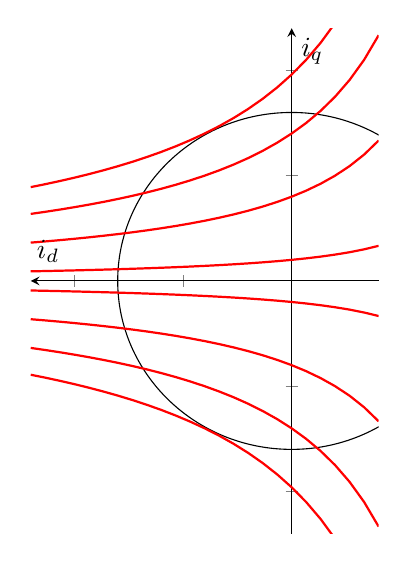
\begin{tikzpicture}
    \begin{axis}[
        axis lines=middle,
        width=6cm,
        height=8cm,
        xlabel={$i_d$},
        x label style={at={(axis description cs:0.05,0.6)},anchor=north},
        ylabel={$i_q$},
        %y label style={at={(axis description cs:0.95,0.05}},
        grid=none,
        xmin=-1.2,
        xmax=0.4,
        ymin=-1.2,
        ymax=1.2,
        no markers,
        x axis line style = {stealth-},
        xticklabels=\empty,  % Elimina las marcas en el eje x
        yticklabels=\empty,  % Elimina las marcas en el eje y
    ]
    
    \draw[black] (0,0) circle [radius=0.8];
    \addplot[red, thick, domain=-1.2:0.4] {4*0.1/(3*2*((2/3)+(2/3)/1*(1-2)*x))};
    \addplot[red, thick, domain=-1.2:0.4] {4*0.4/(3*2*((2/3)+(2/3)/1*(1-2)*x))};
    \addplot[red, thick, domain=-1.2:0.4] {4*0.7/(3*2*((2/3)+(2/3)/1*(1-2)*x))};
    \addplot[red, thick, domain=-1.2:0.4] {4*0.98/(3*2*((2/3)+(2/3)/1*(1-2)*x))};
    
    \addplot[red, thick, domain=-1.2:0.4] {-4*0.1/(3*2*((2/3)+(2/3)/1*(1-2)*x))};
    \addplot[red, thick, domain=-1.2:0.4] {-4*0.4/(3*2*((2/3)+(2/3)/1*(1-2)*x))};
    \addplot[red, thick, domain=-1.2:0.4] {-4*0.7/(3*2*((2/3)+(2/3)/1*(1-2)*x))};
    \addplot[red, thick, domain=-1.2:0.4] {-4*0.98/(3*2*((2/3)+(2/3)/1*(1-2)*x))};
    

    \end{axis}
    \end{tikzpicture}
  \caption{Hipérbolas de par.}
\end{figure}


El gráfico se limita a los cuadrantes 2 y 3 por un motivo ilustrado con estas hipérbolas: solo los valores negativos de \(i_d\) contribuyen a la generación de par en un PMSM con imanes radiales. Cuando \(i_d>0\), se necesita más corriente para generar la misma cantidad de par. Cuanto más alejada está la hipérbola del eje \(i_d\), más par representa en valor absoluto. Aquellas hipérbolas que quedan por encima del eje \(i_d\), es decir, \(i_q > 0\) son par positivo, mientras que si \(i_q < 0\), el par es de sentido opuesto.

\subsubsection{VLE (Elipses de Límite de Voltaje)}

Tomando la ecuación de voltaje \ref{eq_vle_dq}, se puede demostrar que es una elipse. Del mismo modo que con las hipérbolas de par, se pueden establecer una velocidad y una tensión, y deslizar valores de \((i_d, i_q)\) para generar la curva.

\begin{equation}
1 \geq \frac{\left(\frac{\lambda_m}{L_d}+i_d\right)^2}{\left(\frac{\frac{V_{\text{DC}}}{\sqrt{3}}}{L_d\omega_e}\right)^2}+\frac{i_q^2}{\left(\frac{\frac{V_{\text{DC}}}{\sqrt{3}}}{L_q\omega_e}\right)^2}
\end{equation}




\begin{figure}[H]
  \centering
    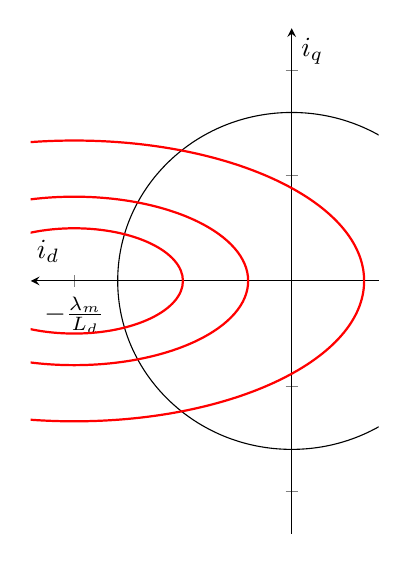
\begin{tikzpicture}
    \begin{axis}[
        axis lines=middle,
        width=6cm,
        height=8cm,
        xlabel={$i_d$},
        x label style={at={(axis description cs:0.05,0.6)},anchor=north},
        ylabel={$i_q$},
        %y label style={at={(axis description cs:0.95,0.05}},
        grid=none,
        xmin=-1.2,
        xmax=0.4,
        ymin=-1.2,
        ymax=1.2,
        no markers,
        x axis line style = {stealth-},
        xtick = {-1},
        xticklabels={$-\frac{\lambda_m}{L_d}$},  % Elimina las marcas en el eje x
        yticklabels=\empty,  % Elimina las marcas en el eje y
    ]
    
    
    \draw[black] (0,0) circle [radius=0.8];
    \draw[red, thick] (-1,0) ellipse (1.333333 and 0.66666666);
    \draw[red, thick] (-1,0) ellipse (0.8 and 0.4);
    \draw[red, thick] (-1,0) ellipse (0.5 and 0.25);

    \end{axis}
    \end{tikzpicture}
  \caption{Elipses de límite de voltaje con $I_{\text{sc}} > I_{s,\text{máx}}$.}
\end{figure}


Al representar estas elipses, normalmente se anotan los valores de velocidad en RPM mecánicas, ya que es mucho más fácil hacerse una idea de los límites del motor junto al resto de curvas (\(\omega_m [\text{RPM}] = \frac{1}{pp} \omega_e \text{ }\left[\frac{\text{rad}}{s}\right] \cdot \frac{60}{2\pi}\)).

Las elipses se reducen a medida que la velocidad aumenta. El foco de las elipses está ubicado exactamente en \((i_d, i_q)=(-I_{\text{sc}}, 0) = \left(-\frac{\lambda_m}{L_d},0\right)\). En el gráfico anterior, el foco está fuera del círculo de límite de corriente, pero no siempre es el caso. Si \(I_{\text{sc}} \leq I_{s,\text{máx}}\), teóricamente el motor puede alcanzar una velocidad infinita, ya que las elipses colapsan en un solo punto. 



\begin{figure}[H]
  \centering
    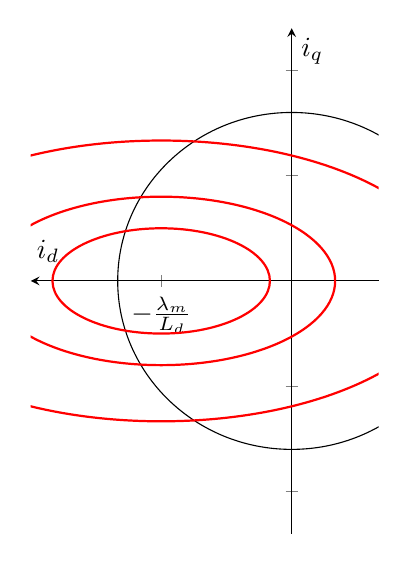
\begin{tikzpicture}
    \begin{axis}[
        axis lines=middle,
        width=6cm,
        height=8cm,
        xlabel={$i_d$},
        x label style={at={(axis description cs:0.05,0.6)},anchor=north},
        ylabel={$i_q$},
        %y label style={at={(axis description cs:0.95,0.05}},
        grid=none,
        xmin=-1.2,
        xmax=0.4,
        ymin=-1.2,
        ymax=1.2,
        no markers,
        x axis line style = {stealth-},
        xtick = {-0.6},
        xticklabels={$-\frac{\lambda_m}{L_d}$},  % Elimina las marcas en el eje x
        yticklabels=\empty,  % Elimina las marcas en el eje y
    ]
    
    
    \draw[black] (0,0) circle [radius=0.8];
    \draw[red, thick] (-0.6,0) ellipse (1.333333 and 0.66666666);
    \draw[red, thick] (-0.6,0) ellipse (0.8 and 0.4);
    \draw[red, thick] (-0.6,0) ellipse (0.5 and 0.25);

    \end{axis}
    \end{tikzpicture}
  \caption{Elipses de límite de voltaje con $I_{\text{sc}} \leq I_{s,\text{máx}}$.}
\end{figure}




%% HASTA AQUI TRACUCCION POCHA DE LA WIKI
\newpage
\section{Control del PMSM en el espacio $d-q$}
\subsection{Trayectorias de control}

Después de conocer los límites de la máquina, se pueden establecer criterios para decidir cuánto \(i_d\) y \(i_q\) (o \(i_s\) y \(\gamma\)) se deben aplicar al PMSM para que se comporte mecánicamente como se desee. El conjunto de puntos de trabajo que definen un comportamiento se llama trayectoria y existen una multitud de ellas. Por ejemplo, se puede desear que el motor produzca la mayor cantidad de par posible con la mínima corriente. Pero también se podría querer que tenga un cierto factor de potencia o que mantenga el par constante subiendo la velocidad, etc.

En un monoplaza de Formula Student, se desea que la salida de par esté perfectamente controlada y conocida para que el algoritmo de dinámica vehicular pueda estimar correctamente las fuerzas en los neumáticos. También es deseable que el motor pueda girar más rápido cuando no se requiere más par, ya que no es necesaria mucha tracción a altas velocidades del vehículo. Además, es necesario que sea eficiente para aprovechar mejor la energía de la batería. Con estos requisitos en mente, se estudian 4 trayectorias de control adecuadas para esta aplicación.

\subsubsection{MTPA (Máximo Par Por Amperio)}

La trayectoria de control más utilizada es el MTPA, o Máximo Par Por Amperio. Como su nombre indica, minimiza la corriente para entregar un par determinado. La condición que se debe cumplir es

\begin{equation}
	\frac{\partial T_{\text{em}}}{\partial \gamma} = 0 \text{ .}
\end{equation}


La expresión analítica se desarrolla partiendo de la ecuación de par en forma polar \ref{eq_tq_pol},

\begin{equation*}
	T_{\text{em}} = \frac{3}{2}pp\cdot((L_d - L_q)\cdot i_s^2 \cdot \sin(\gamma)\cos(\gamma) + \lambda_m\cdot i_s\cdot \sin(\gamma))
\end{equation*}


\begin{equation}
\frac{\partial T_{\text{em}}}{\partial \gamma} = \frac{\partial}{\partial \gamma} \frac{3}{2}pp\cdot(i_s^2 \cos(\gamma)\sin(\gamma)\cdot((L_d - L_q) + \lambda_m i_s \sin(\gamma)) = 0
\end{equation}

\begin{equation}
 \therefore i_{s,\text{MTPA}} = -\frac{\lambda_m \cos(\gamma)}{(2\cdot\cos(\gamma)^2 - 1)\cdot(L_d-L_q)} \text{ .}
\end{equation}

Para la aplicación de esta trayectoria en el control se busca el ángulo como función de la corriente, y para ello se debe despejar \(\gamma_{\text{MTPA}}\) de la expresión.

\begin{equation}
\gamma_{\text{MTPA}} = \frac{\pi}{2} + \arcsin\left( \frac{\lambda_m - \sqrt{8(L_d-L_q)^2 \cdot i_s^2 + \lambda_m^2}}{4\cdot i_s(L_d-L_q)}\right) 
\end{equation}

El resultado de graficar esta expresión sobre el plano \((i_d, i_q)\) deja a la vista que el módulo de corriente es mínimo para cada hipérbola de par.


\begin{figure}[H]
  \centering
    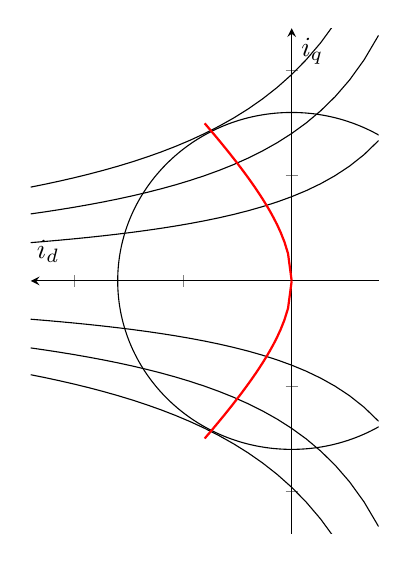
\begin{tikzpicture}
    \begin{axis}[
        axis lines=middle,
        width=6cm,
        height=8cm,
        xlabel={$i_d$},
        x label style={at={(axis description cs:0.05,0.6)},anchor=north},
        ylabel={$i_q$},
        %y label style={at={(axis description cs:0.95,0.05}},
        grid=none,
        xmin=-1.2,
        xmax=0.4,
        ymin=-1.2,
        ymax=1.2,
        no markers,
        x axis line style = {stealth-},
        xticklabels=\empty,  % Elimina las marcas en el eje x
        yticklabels=\empty,  % Elimina las marcas en el eje y
    ]
    
    \draw[black] (0,0) circle [radius=0.8];
    \addplot[black, domain=-1.2:0.4] {4*0.4/(3*2*((2/3)+(2/3)/1*(1-2)*x))};
    \addplot[black, domain=-1.2:0.4] {4*0.7/(3*2*((2/3)+(2/3)/1*(1-2)*x))};
    \addplot[black, domain=-1.2:0.4] {4*0.98/(3*2*((2/3)+(2/3)/1*(1-2)*x))};
    
    \addplot[black, domain=-1.2:0.4] {-4*0.4/(3*2*((2/3)+(2/3)/1*(1-2)*x))};
    \addplot[black, domain=-1.2:0.4] {-4*0.7/(3*2*((2/3)+(2/3)/1*(1-2)*x))};
    \addplot[black, domain=-1.2:0.4] {-4*0.98/(3*2*((2/3)+(2/3)/1*(1-2)*x))};
    
    \addplot[red, thick, domain=-0.4:0] {sqrt(((2/3)*x+(2/3)*(1-2)*x^2)/((2/3)*(1-2))))};
    \addplot[red, thick, domain=-0.4:0] {-sqrt(((2/3)*x+(2/3)*(1-2)*x^2)/((2/3)*(1-2))))};


    \end{axis}
    \end{tikzpicture}
  \caption{Trayectoria MTPA.}
\end{figure}


\subsubsection{CTC (Curva de Par Constante)}

Como se puede observar, las hipérbolas de par definen una trayectoria la cual permite mantener un par constante. Recordando las elipses de tensión, para un mismo valor de $V_s$ las elipses se contraen hacia el foco a medida que la velocidad aumenta. Esto significa que siguiendo la curva de par constante de derecha a izquierda se puede mantener el par aumentando la velocidad. Usando la expresión \ref{eq_tq_pol} se puede obtener directamente 
\begin{equation*}
	T_{\text{em}} = \frac{3}{2}pp\cdot((L_d - L_q)\cdot i_s^2 \cdot \sin(\gamma)\cos(\gamma) + \lambda_m\cdot i_s\cdot \sin(\gamma))
\end{equation*}

\begin{equation}
 \therefore i_{s,\text{CTC}} = \frac{\lambda_m}{L_d} \cdot \frac{\sqrt{\sin(\gamma)^2+\frac{4\cdot\frac{L_d-L_q}{L_d}\cdot\sin(2\gamma)\cdot T_{\text{em}}\cdot L_d}{3\cdot pp \cdot \lambda_m^2}}-\sin(\gamma)}{\sin(2\gamma)\cdot(\frac{L_d-L_q}{L_d})} \text{ .}
\end{equation}



\begin{figure}[H]
  \centering
    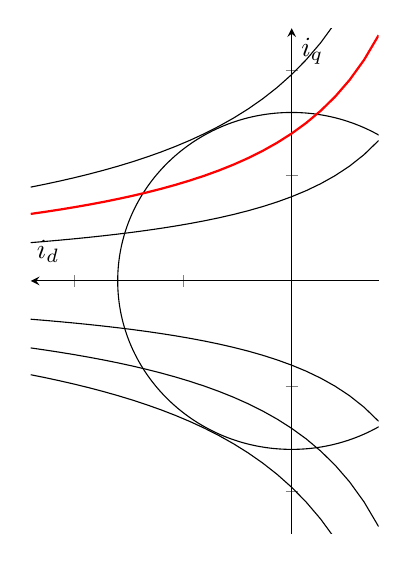
\begin{tikzpicture}
    \begin{axis}[
        axis lines=middle,
        width=6cm,
        height=8cm,
        xlabel={$i_d$},
        x label style={at={(axis description cs:0.05,0.6)},anchor=north},
        ylabel={$i_q$},
        %y label style={at={(axis description cs:0.95,0.05}},
        grid=none,
        xmin=-1.2,
        xmax=0.4,
        ymin=-1.2,
        ymax=1.2,
        no markers,
        x axis line style = {stealth-},
        xticklabels=\empty,  % Elimina las marcas en el eje x
        yticklabels=\empty,  % Elimina las marcas en el eje y
    ]
    
    \draw[black] (0,0) circle [radius=0.8];
    \addplot[black, domain=-1.2:0.4] {4*0.4/(3*2*((2/3)+(2/3)/1*(1-2)*x))};
    \addplot[red, thick, domain=-1.2:0.4] {4*0.7/(3*2*((2/3)+(2/3)/1*(1-2)*x))};
    \addplot[black, domain=-1.2:0.4] {4*0.98/(3*2*((2/3)+(2/3)/1*(1-2)*x))};
    
    \addplot[black, domain=-1.2:0.4] {-4*0.4/(3*2*((2/3)+(2/3)/1*(1-2)*x))};
    \addplot[black, domain=-1.2:0.4] {-4*0.7/(3*2*((2/3)+(2/3)/1*(1-2)*x))};
    \addplot[black, domain=-1.2:0.4] {-4*0.98/(3*2*((2/3)+(2/3)/1*(1-2)*x))};
    
    \end{axis}
    \end{tikzpicture}
  \caption{Trayectoria CTC.}
\end{figure}


\subsubsection{MTPV (Máximo Par Por Voltio)}

Existe una trayectoria que permite maximizar el par entregado por el motor en rangos de velocidad muy altos donde el límite es la tensión que puede sintetizar la controladora. La condición que se debe cumplir es que

\begin{equation}
\frac{\partial T_{\text{em}}}{\partial \delta} = 0 \text{.}
\end{equation}

Donde $\delta$ es el ángulo del vector de tensión $V_s$, de la misma manera que $\gamma$ es el ángulo del vector de corriente $I_s$. La expresión analítica se desarrolla a partir de la expresión de par en coordenadas cartesianas (\ref{eq_tq_dq}), de manera que

\begin{equation*}
T_{\text{em}} = \frac{3}{2}pp\cdot((L_d - L_q) i_q i_d + \lambda_m i_q) \text{ .}
\end{equation*}

Se aíslan $i_d$ e $i_q$ de \ref{eq_vd} y \ref{eq_vq}, negligiendo la caída de tensión resistiva del estátor, 
\begin{equation}
i_d = \frac{v_q}{\omega_e \cdot L_d} - \frac{\lambda_m}{L_d}; i_q = -\frac{v_d}{\omega_e \cdot L_q}
\end{equation}

\begin{equation}
T_{\text{em}} = \frac{3}{2}pp\cdot\left((L_d - L_q) (-\frac{v_d}{\omega_e \cdot L_q}) (\frac{v_q}{\omega_e \cdot L_d} - \frac{\lambda_m}{L_d}) + \lambda_m (-\frac{v_d}{\omega_e \cdot L_q})\right)
\end{equation}

\begin{equation}
 T_{\text{em}} = \frac{3}{2}pp\cdot\left((L_d - L_q) (-\frac{V_s \cdot \cos(\delta)}{\omega_e \cdot L_q}) (\frac{V_s \cdot \sin(\delta)}{\omega_e \cdot L_d} - \frac{\lambda_m}{L_d}) + \lambda_m (-\frac{V_s \cdot \cos(\delta)}{\omega_e \cdot L_q})\right)
\end{equation}

\begin{equation}
\begin{split}
 \therefore \frac{\partial T_{\text{em}}}{\partial \delta} = \frac{3}{2}pp\cdot (
(L_d - L_q) \cdot (\frac{V_s \cdot \sin(\delta)}{\omega_e \cdot L_q}) \cdot (\frac{V_s \cdot \sin(\delta)}{\omega_e \cdot L_d} - \frac{\lambda_m}{L_d})\\
-\left(\frac{V_s \cdot \cos(\delta)}{\omega_e}\right)^2 \cdot \frac{L_d - L_q}{L_d\cdot L_q}\\ 
-\frac{\lambda_m \cdot V_s \cdot \sin(\delta)}{L_q \cdot \omega_e} ) = 0  \text{ .}
\end{split}
\end{equation}

Definiendo la saliencia  
\begin{equation}
	\xi = \frac{L_q}{L_d}
\end{equation}

y aislando, se obtiene
\begin{equation}
\begin{split}
i_{s,\text{MTPV}} = \frac{\lambda_m}{L_d} ( \frac{-(2 - \xi) \cos(\gamma)}{2(1 - \xi)(1 + (\xi)^2) \cos(\gamma)^2 - 2(1 - \xi) (\xi)^2}\\
-\frac{\sqrt{(2 - \xi)^2 \cos(\gamma)^2 - 4(1 - \xi)(1 + (\xi)^2) \cos(\gamma)^2 - 4(1 - \xi) (\xi)^2}}{2(1 - \xi)(1 + (\xi)^2) \cos(\gamma)^2 - 2(1 - \xi) (\xi)^2} )  \text{ .}
\end{split}
\end{equation}




Cabe destacar que esta trayectoria solamente se puede ejecutar si se cumple la condición de que $I_{\text{sc}} \leq I_{s,\text{máx}}$.


\begin{figure}[H]
  \centering
    \begin{tikzpicture}
    \begin{axis}[
        axis lines=middle,
        width=6cm,
        height=8cm,
        xlabel={$i_d$},
        x label style={at={(axis description cs:0.05,0.6)},anchor=north},
        ylabel={$i_q$},
        %y label style={at={(axis description cs:0.95,0.05}},
        grid=none,
        xmin=-1.2,
        xmax=0.4,
        ymin=-1.2,
        ymax=1.2,
        no markers,
        x axis line style = {stealth-},
        xtick = {-0.6},
        xticklabels={$-\frac{\lambda_m}{L_d}$},  % Elimina las marcas en el eje x
        yticklabels=\empty,  % Elimina las marcas en el eje y
    ]
    
    
    \draw[black] (0,0) circle [radius=0.8];
    \addplot[red, thick, domain=-0.77:-0.6] {0.5*sqrt(4*(1.111111)^2*(x^2-x*0)+(1.111111)^2*0^2-2.22222222^2*0.6^2)/2.22222222};


    \end{axis}
    \end{tikzpicture}
  \caption{Trayectoria MTPV.}
\end{figure}



\subsubsection{CVL (Límites de Corriente y Voltaje)}

Por último, se presentan los límites eléctricos del motor y del convertidor. El límite de corriente consiste simplemente en saturar la magnitud de la corriente de manera que no sobrepase el valor máximo establecido. La trayectoria sería sencillamente seguir el círculo de corriente anteriormente presentado (CLC), con la siguiente expresión:

\[
i_{s,\text{CLC}} = I_{s,\text{máx}} , \forall \gamma \in [0,2\pi]
\]


\begin{figure}[H]
  \centering
    \begin{tikzpicture}
    \begin{axis}[
        axis lines=middle,
        width=6cm,
        height=8cm,
        xlabel={$i_d$},
        x label style={at={(axis description cs:0.05,0.6)},anchor=north},
        ylabel={$i_q$},
        %y label style={at={(axis description cs:0.95,0.05}},
        grid=none,
        xmin=-1.2,
        xmax=0.4,
        ymin=-1.2,
        ymax=1.2,
        no markers,
        x axis line style = {stealth-},
        xticklabels=\empty,  % Elimina las marcas en el eje x
        yticklabels=\empty,  % Elimina las marcas en el eje y
    ]
    
    % Límite de corriente Is_max
    \draw[red, thick] (0,0) circle [radius=0.8];

    \end{axis}
    \end{tikzpicture}
  \caption{Trayectoria CLC.}
\end{figure}


El límite de tensión del motor en realidad se puede entender como la velocidad máxima a la que se puede llegar con una determinada tensión. Por ello, se usa la forma polar de la expresión de las elipses de tensión (VLE),

\begin{equation}
1 \geq \frac{\left(\frac{\lambda_m}{L_d}+i_s \cdot \cos(\gamma)\right)^2}{\left(\frac{\frac{V_{\text{DC}}}{\sqrt{3}}}{L_d\cdot\omega_e}\right)^2}+\frac{(i_s \cdot \sin(\gamma))^2}{\left(\frac{\frac{V_{\text{DC}}}{\sqrt{3}}}{L_q\cdot\omega_e}\right)^2} \text{.}
\end{equation}

Igual que para el resto de trayectorias, se debe obtener una expresión de la elipse en función de $I_s$ y $\gamma$. Ya que no es trivial despejar estas variables de la expresión anterior, se manipula usando la ecuación polar de la elipse desplazada del origen, de manera que
\begin{equation}
\rho(\theta) = \frac{b^2 x \cos (\theta ) + a^2 y \sin (\theta )\pm a b \sqrt{\left(a^2-x^2\right) \sin ^2(\theta )+\left(b^2-y^2\right) \cos ^2(\theta )+2 x y \sin (\theta ) \cos (\theta )}}{a^2 \sin ^2(\theta )+b^2 \cos ^2(\theta )} \text{.}
\end{equation}

Dado que estas elipses tan solo están desplazadas en el eje $x$, se pueden eliminar todos los términos referentes al desplazamiento en $y$.
\begin{equation}
\rho(\theta) = \frac{b^2 x \cos (\theta ) \pm a b \sqrt{\left(a^2-x^2\right) \sin ^2(\theta )+\left(b^2\right) \cos ^2(\theta )}}{a^2 \sin ^2(\theta )+b^2 \cos ^2(\theta )}
\end{equation}

Sustituyendo por los términos conocidos y simplificando,

\begin{equation}
	i_{s,\text{VLE}} =\frac{\left(\frac{1}{L_q}\right)^2\left(-I_{s c}\right) \cos (\gamma) \pm \frac{1}{L_d \cdot L_q} \sqrt{\left(\left(\frac{V_s}{L_d \cdot \omega_e}\right)^2-\left(-I_{s c}\right)^2\right) \sin ^2(\gamma)+\left(\frac{V_s}{L_q \cdot \omega_e}\right)^2 \cos ^2(\gamma)}}{\left(\frac{1}{L_d}\right)^2 \sin ^2(\gamma)+\left(\frac{1}{L_q}\right)^2 \cos ^2(\gamma)} \text{.}
\end{equation}


\begin{figure}[H]
  \centering
    \begin{tikzpicture}
    \begin{axis}[
        axis lines=middle,
        width=6cm,
        height=8cm,
        xlabel={$i_d$},
        x label style={at={(axis description cs:0.05,0.6)},anchor=north},
        ylabel={$i_q$},
        %y label style={at={(axis description cs:0.95,0.05}},
        grid=none,
        xmin=-1.2,
        xmax=0.4,
        ymin=-1.2,
        ymax=1.2,
        no markers,
        x axis line style = {stealth-},
        xtick = {-1},
        xticklabels={$-\frac{\lambda_m}{L_d}$},  % Elimina las marcas en el eje x
        yticklabels=\empty,  % Elimina las marcas en el eje y
    ]
    
    
    \draw[black] (0,0) circle [radius=0.8];

    \draw[red, thick] (-1,0) ellipse (0.5 and 0.25);


    \end{axis}
    \end{tikzpicture}
  \caption{Trayectoria VLE.}
\end{figure}



Además, el inversor es capaz de sintetizar un máximo de $V_s = \frac{V_{\text{DC}}}{\sqrt{3}}$ utilizando SVPWM, por lo tanto, se debe saturar la consigna de tensión a ese valor. Adicionalmente, por seguridad, se multiplica por un factor de seguridad $K_{\text{FW}} \in (0,1)$.

\begin{equation}
	V_{s,\text{máx}} \leq \frac{V_{\text{DC}}}{\sqrt{3}}\cdot K_{\text{FW}}
\end{equation}

\subsection{Diseño y simulación del control}

En esta sección, se aborda la implementación del modelo matemático del PMSM en un entorno de simulación. Además, se detallan los pasos cruciales en el diseño del control, destacando la implementación del lazo de control de corriente, el modelo promediado y conmutado del inversor, o la integración de las trayectorias y la estrategia de debilitamiento de campo. Disponer de un modelo de simulación completo permite ganar mucha comprensión sobre el sistema estudiado, pero por el coste computacional suele ser inviable juntar muchos sistemas en una misma simulación.

\subsubsection{EMR (Representación macroscópica energética)}
En primer lugar, se creará un modelo que permita simular la dinámica electromecánica del PMSM, así como los entornos mecánico (vehículo) y eléctrico (batería) en los que se encuentra, para posteriormente integrar el control vectorial. Para ello se usará un estándar para modelizar sistemas de potencia, la representación macroscópica energética o EMR por sus siglas en inglés \cite{6387385}. El concepto se basa en agrupar o dividir las diferentes etapas en las que la potencia se transforma, utilizando el principio de acción-reacción y el principio causal (el efecto causa-efecto causa efecto porque la causa del efecto causa-efecto es a su vez causa y efecto \cite{causaEfecto}). 


\begin{figure}[H]
	\centering
	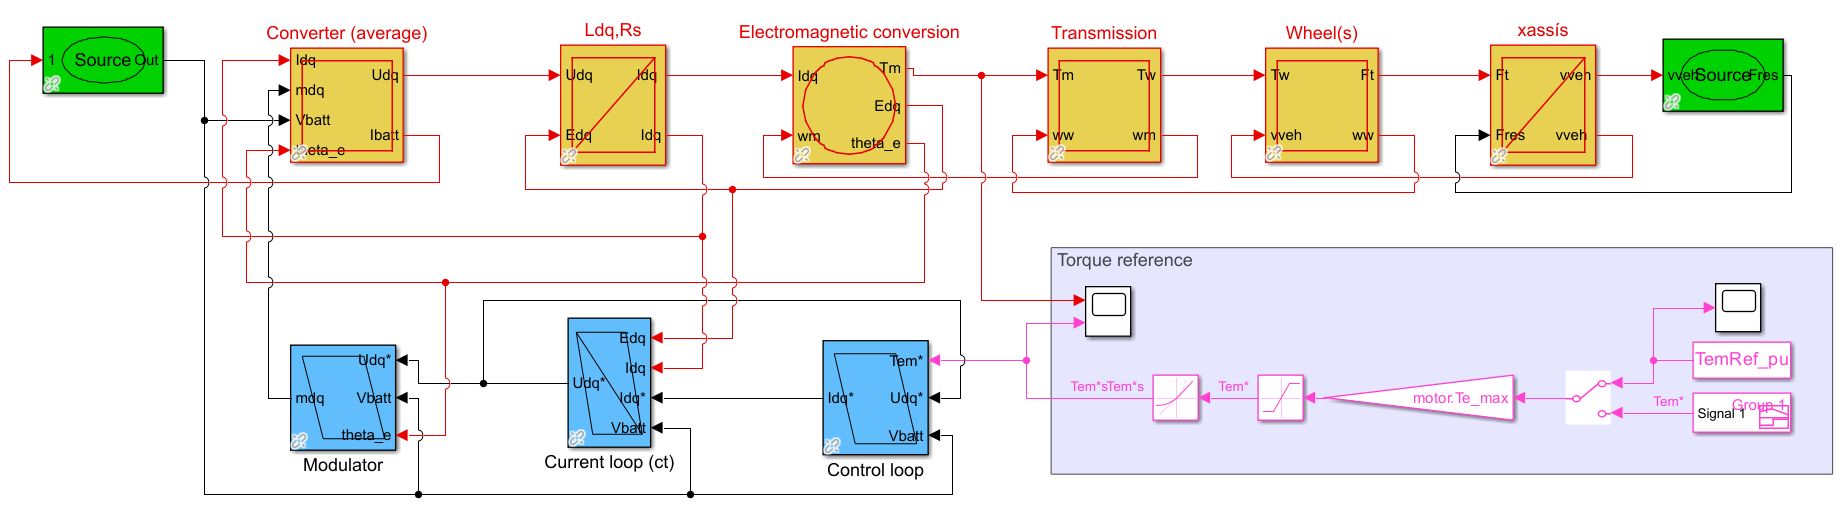
\includegraphics[width=1\linewidth]{fig/EMR_FULL.png}
	\caption{Modelo EMR completo.}
\end{figure}

En primer lugar se modeliza la planta eléctrica del PMSM. Se utiliza el modelo con el marco de referencia rotativo $d-q$ por su sencillez. Para ello se implementan las diferentes ecuaciones del motor en bloques separados siguiendo el estándar de la EMR.

\begin{figure}[H]
    \centering
    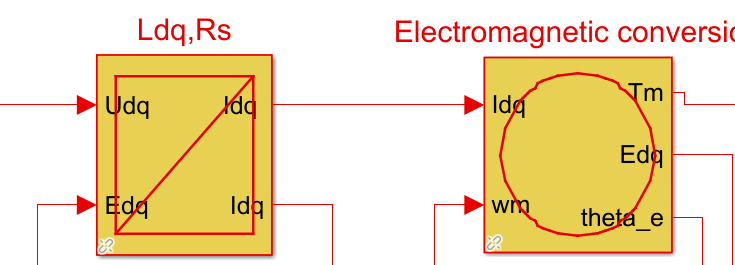
\includegraphics[width=0.7\linewidth]{fig/motorEMR1.png}
    \caption{Bloques que representan el PMSM.}
\end{figure}

También se modela la planta mecánica del motor, así como la transmisión de la potencia mecánica a las ruedas y al vehículo.

\begin{figure}[H]
    \centering
    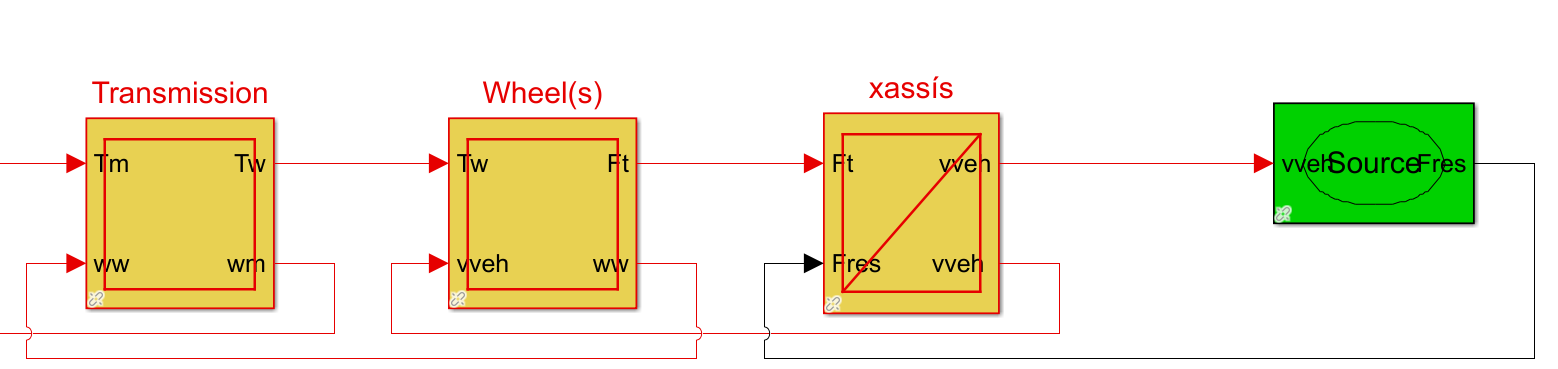
\includegraphics[width=0.95\linewidth]{fig/carEMR.png}
    \caption{Planta mecánica.}
\end{figure}

\subsubsection{Parámetros y curvas del PMSM simulado}

A fecha de redacción de este documento no se han obtenido los parámetros del motor utilizado por el equipo. Sin embargo, se han estimado usando un pequeño \textit{script} de MATLAB de manera que se cumplan los requisitos de potencia del motor.

\begin{table}[H]
	\begin{tabular}{|p{2cm}||r|p{1.5cm}|p{8cm}|}
		\hline
		\multicolumn{4}{|c|}{Parámetros del motor} \\
		\hline
		Parámetro & Valor & Unidades & Descripción \\
		\hline
		pp & 3 & ad & Número de pares de polos \\
		$\lambda_m$ & 52,615 & mWb & Flujo magnético de los imanes permanentes \\
		$L_d$ & 188,7 & \unit{\micro\henry} & Inductancia en el eje d \\
		$L_q$ & 283,1 & \unit{\micro\henry} & Inductancia en el eje q \\
		$R_s$ & 150 & m$\Omega$ & Resistencia de fase del estátor \\
		$\omega_{\text{m,máx}}$ & 20000 & RPM & Velocidad angular máxima del motor \\
		$T_{\text{em,máx}}$ & 26 & N·m & Par máximo del motor \\
		\(V_{\text{DC,máx}}\) & 600 & \unit{V} & Voltaje máximo DC \\
		$I_{\text{s,máx}}$ & 108 & A & Corriente máxima en los ejes d-q \\
		\hline
	\end{tabular}
	\caption{Parámetros del PMSM simulado.}
\end{table}

Como se puede ver, el motor presenta $I_{\text{sc}} = \frac{\lambda_m}{L_d} =  \frac{52.615 \text{ mWb}}{188.7 \text{ }\text{\unit{\micro\henry}}} = 278.82 \text{ A} > I_{s,\text{máx}}$, y por tanto, no se aplica la trayectoria MTPV. Esto se comprueba graficando las curvas del motor, mostradas en la figura \ref{curvasmotor}.

\begin{figure}[H]
	\centering
	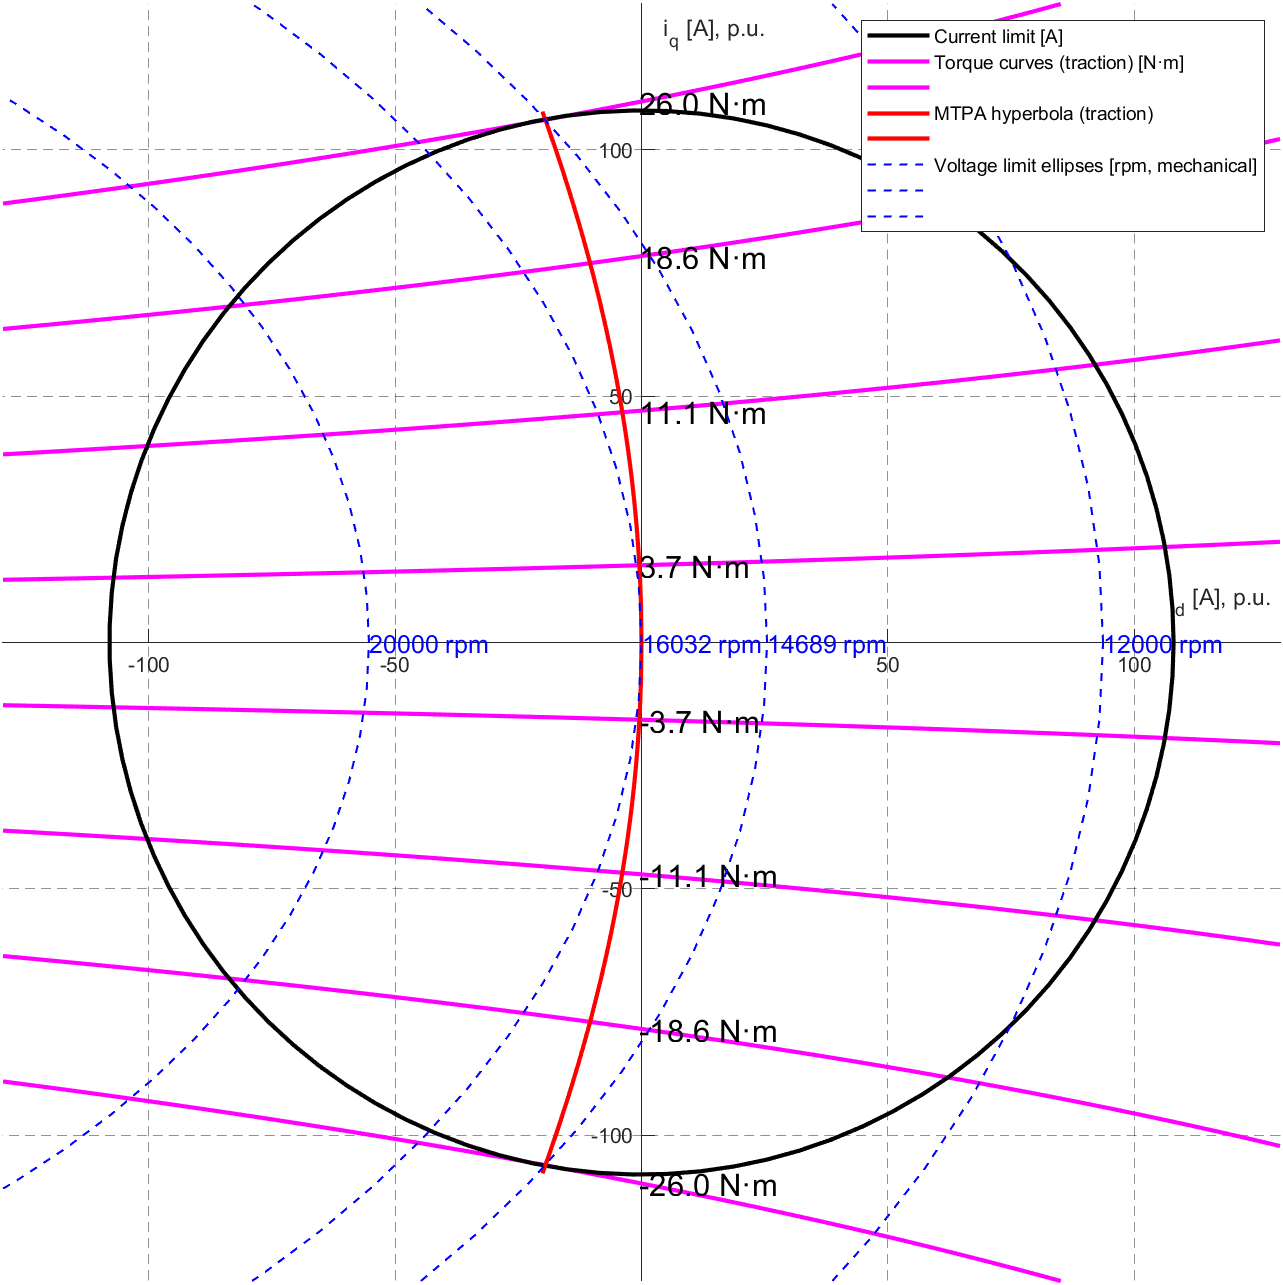
\includegraphics[width=0.7\linewidth]{fig/curvasMotor}
	\caption{Gráfico de las curvas características del PMSM simulado.}
	\label{curvasmotor}
\end{figure}

\subsubsection{Lazos de corriente y modelo promediado del inversor}

Como se ha visto hasta ahora, es práctico utilizar la corriente para controlar el motor. Por ello, se implementa un lazo de corriente utilizando controladores PI para el eje $d$ y para el eje $q$ por separado. Como el inversor se utiliza como fuente de tensión, la salida de estos PI es la consigna de tensión. Dado que el motor genera una fuerza contraelectromotriz, se añade como \textit{feed-forward} a los controladores. La salida del controlador no se satura directamente, sino que se implementa una saturación posterior la cual se realimenta al controlador para usar una técnica de \textit{anti-windup} propuesta en \cite{chandana2002}. Las constantes de los controladores se ajustan de la siguiente manera:

% PI de corriente, respuesta de segundo orden
\[
M_p = 15 \%
\]

\[
 t_s = T_s \cdot 20
\]
Donde $M_p$ es el sobre-impulso deseado en la respuesta a una entrada de escalón, $t_s$ es el tiempo de establecimiento deseado, y $T_s$ es la inversa de la frecuencia de control.

\begin{equation}
	\xi = \sqrt{\frac{\log(M_p)^2}{\pi^2 + \log(M_p)^2}}
\end{equation}

\begin{equation}
\omega_n = \frac{3}{\xi \cdot t_s}
\end{equation}

\begin{equation}
Kp_{id} = 2 \cdot \xi \cdot \omega_n \cdot L_d - R_s
\end{equation}

\begin{equation}
Ki_{id} = \omega_n^2 \cdot L_d
\end{equation}

\begin{equation}
Kp_{iq} = 2 \cdot \xi \cdot \omega_n \cdot L_q - R_s
\end{equation}

\begin{equation}
Ki_{iq} = \omega_n^2 \cdot L_q \quad
\end{equation}

\begin{figure}[H]
    \begin{subfigure}{0.2\linewidth}
        \centering
        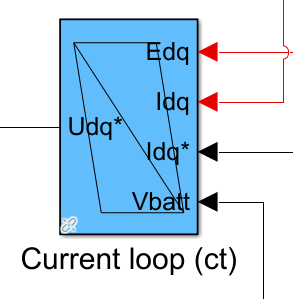
\includegraphics[width=\linewidth]{fig/PIEMR_out.png}
    \end{subfigure}
    \begin{subfigure}{0.75\linewidth}
        \centering
        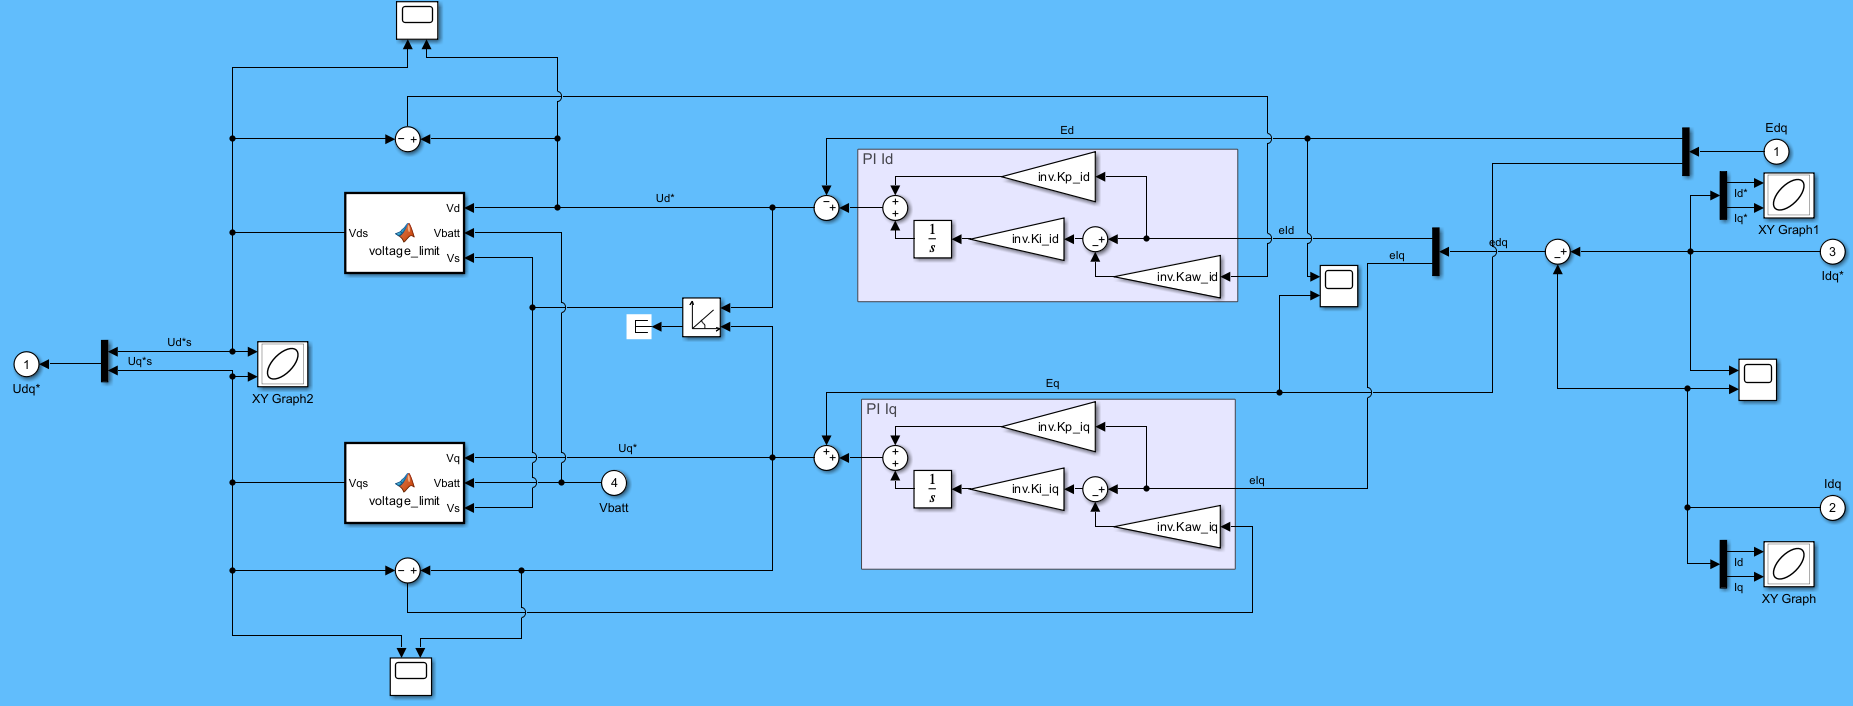
\includegraphics[width=\linewidth]{fig/PIEMR_in.png}
    \end{subfigure}
    \caption{Bloque de los lazos de corriente.}
\end{figure}

\begin{figure}[H]
    \centering
    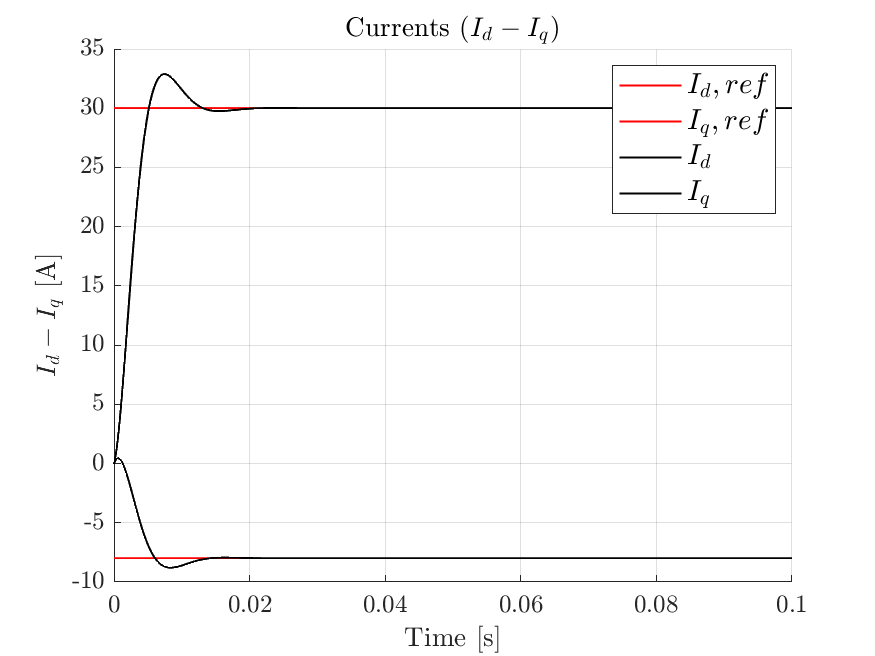
\includegraphics[width=0.75\linewidth]{fig/idiq_plot_PI.png}
    \caption{Simulación de los lazos de corriente, con una consigna de $(i_d, i_q) = (-8, 30) \text{ A}$.}
\end{figure}


Tras obtener las consignas de tensión, se modela el inversor VSI con SVPWM con un modelo promediado, es decir, sin llegar a generar una señal conmutada por PWM. Se usan relaciones básicas para convertir las magnitudes eléctricas del espacio $d-q$ a DC. Además se incorpora la fuente de energía del sistema, la batería, con un simple modelo RC.

\begin{figure}[H]
    \centering
    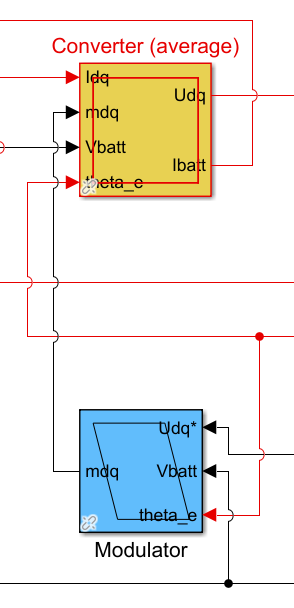
\includegraphics[width=0.25\linewidth]{fig/VSIEMR_out.png}
    \caption{Bloques que contienen el modelo promediado del VSI con SVPWM.}

\end{figure}

\begin{figure}[H]
    \centering
    \begin{subfigure}{0.45\linewidth}
        \centering
        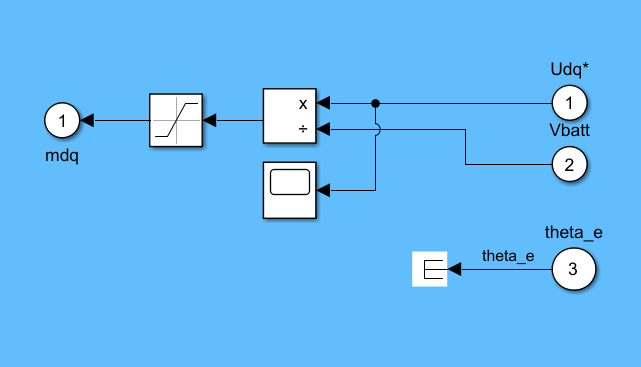
\includegraphics[width=\linewidth]{fig/VSIEMR_in1.png}
    \end{subfigure}
    \begin{subfigure}{0.45\linewidth}
        \centering
        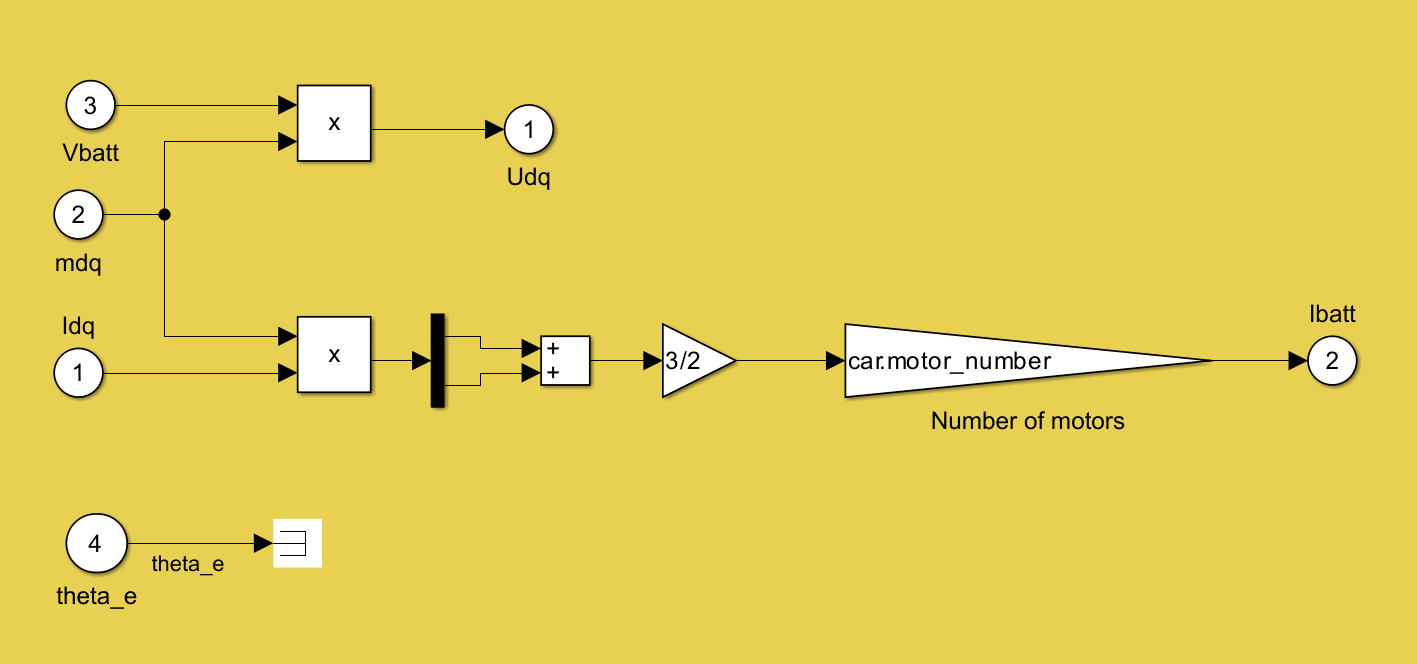
\includegraphics[width=\linewidth]{fig/VSIEMR_in2.png}
    \end{subfigure}
    \caption{Detalle de los bloques del VSI.}

\end{figure}

\subsubsection{Implementación de las trayectorias de control}

Con lo anteriormente desarrollado solamente se pueden consignar las corrientes $i_d$ e $i_q$ manualmente, pero el objetivo es consignar el par y que el propio control sea capaz de gestionar el debilitamiento de campo. Por ello, se implementan las ecuaciones presentadas en el apartado anterior en bloques de código. El control se ha basado en la propuesta de \cite{carlos2023}.

La estrategia es la siguiente: Se implementan las ecuaciones de las trayectorias cuya salida es una corriente (CLC, CTC y MTPV) y se selecciona la mínima. En paralelo, se calcula el ángulo que correspondería a la trayectoria del MTPA, y se añade un control integral que aumenta el valor del ángulo controlando la tensión para poder entrar en el resto de trayectorias. Este integrador sería justamente el controlador de debilitamiento de campo y se encarga de que la consigna de ángulo no haga sobrepasar el límite de tensión establecido por el bus DC con un cierto factor de seguridad. Se trabaja con módulos de corriente siempre positivos, y ángulos comprendidos entre $\gamma \in [\frac{\pi}{2}, \pi]$. Para obtener par negativo (regeneración), simplemente se multiplica el ángulo $\gamma$ por el signo de la consigna de par, atendiendo específicamente al caso de par igual a cero.


\begin{figure}[H]
    \centering
    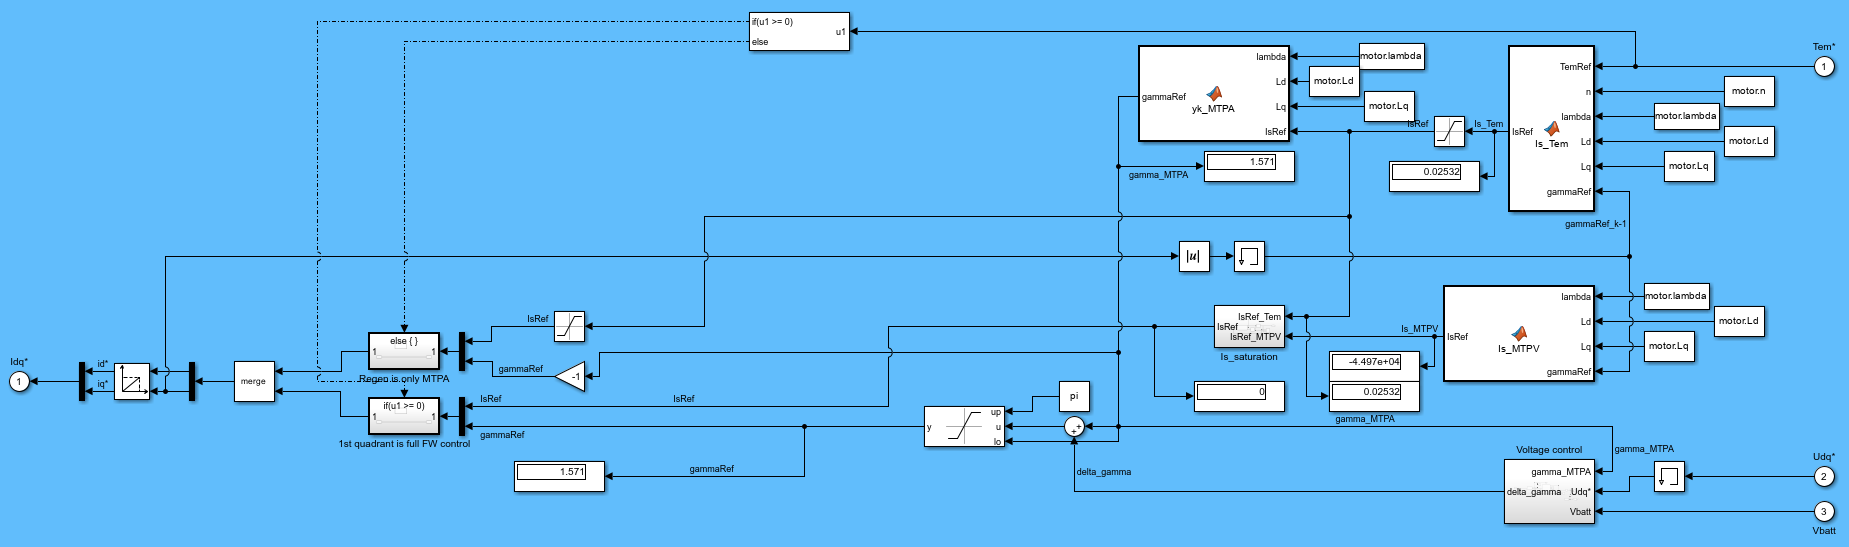
\includegraphics[width=1\linewidth]{fig/EMR_control.png}
    \caption{Detalle del bloque del lazo de control vectorial.}
    
\end{figure}
\newpage

Para comprobar el funcionamiento y la estabilidad del control, se realiza una simulación en la que la consigna de par está extraída de un perfil de conducción real.

\begin{figure}[!htb]
    \centering
    \begin{subfigure}{0.4\textwidth}
        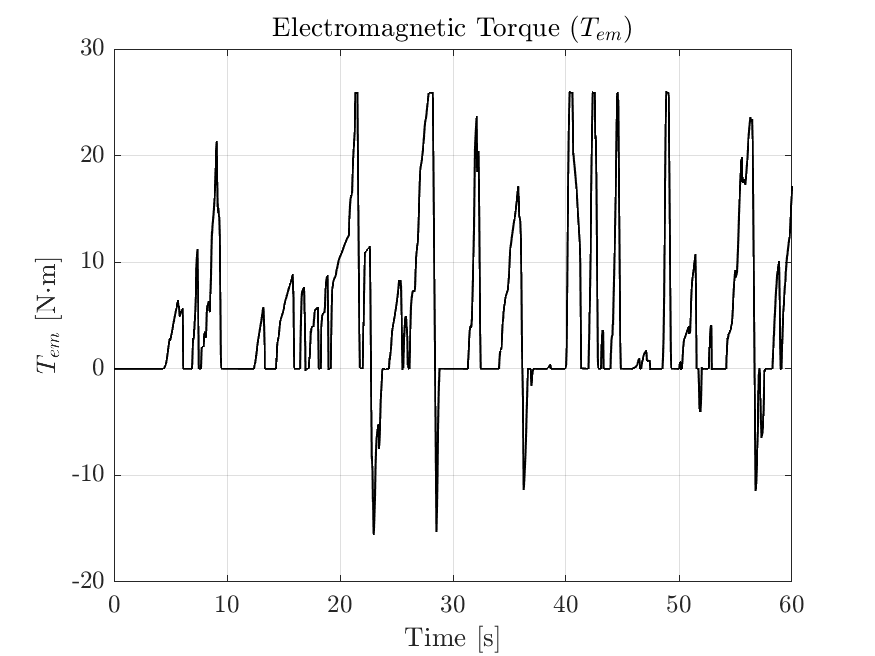
\includegraphics[width=\linewidth]{fig/Tem_plot.png}
        \caption{Par electromagnético generado por el motor ($T_{\text{em}}$).}
    \end{subfigure}
    \begin{subfigure}{0.4\textwidth}
        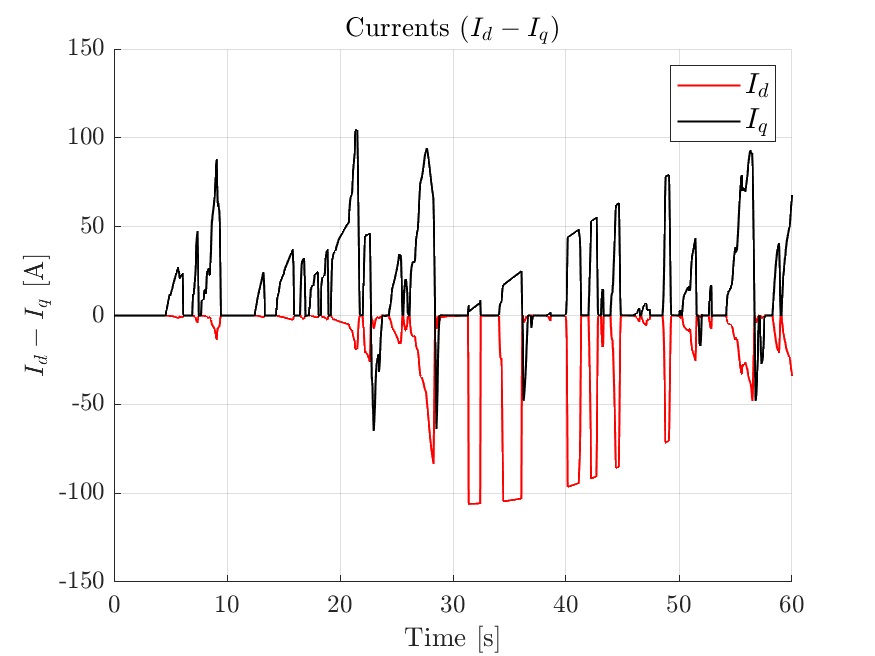
\includegraphics[width=\linewidth]{fig/idiq_plot.png}
        \caption{Corrientes ($I_{d} - I_{q}$).}
    \end{subfigure}
    \begin{subfigure}{0.4\textwidth}
        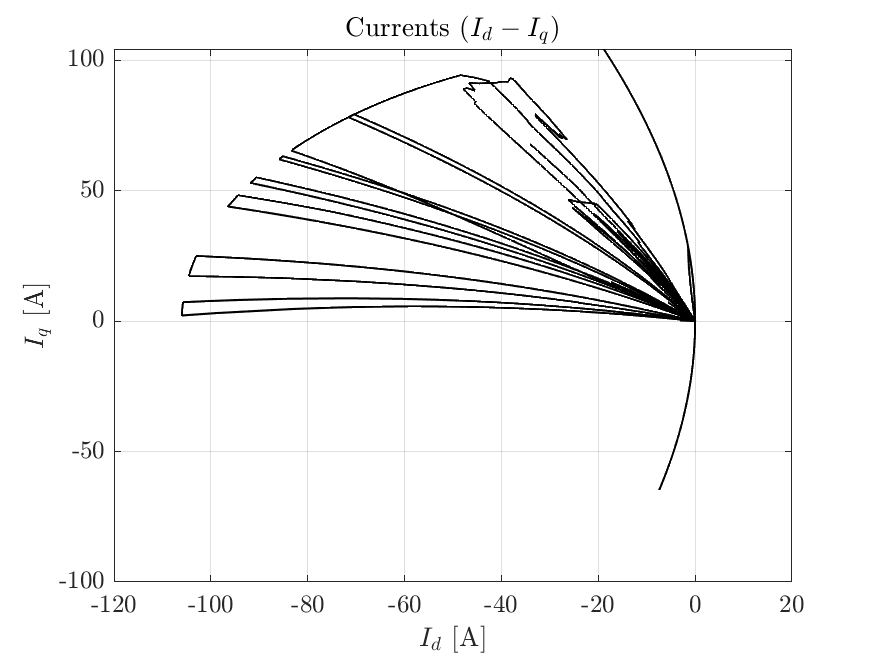
\includegraphics[width=\linewidth]{fig/id-iq_plot.png}
        \caption{Corriente ($I_{d}$) vs Corriente ($I_{q}$).}
    \end{subfigure}
    \begin{subfigure}{0.4\textwidth}
        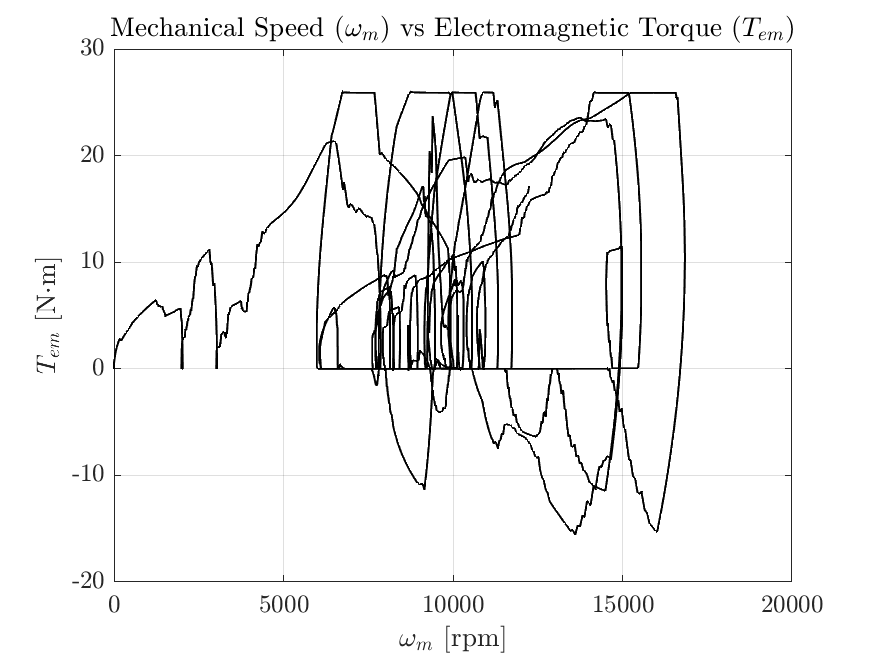
\includegraphics[width=\linewidth]{fig/wm_Tem_plot.png}
        \caption{Velocidad mecánica ($\omega_{m}$) vs Par electromagnético ($T_{\text{em}}$).}
    \end{subfigure}
    \begin{subfigure}{0.4\textwidth}
        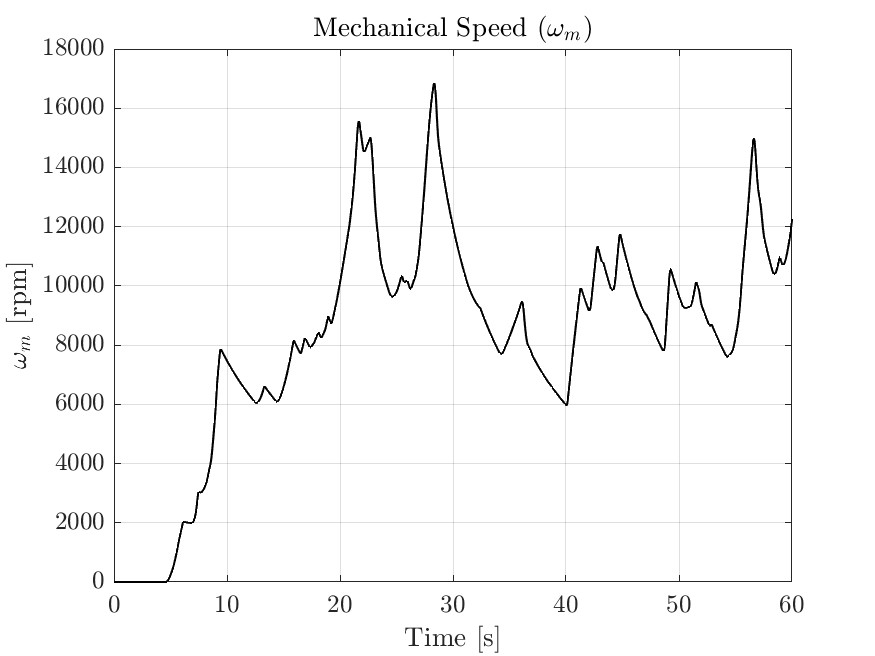
\includegraphics[width=\linewidth]{fig/wm_plot.png}
        \caption{Velocidad mecánica ($\omega_{m}$).}
    \end{subfigure}
    \begin{subfigure}{0.4\textwidth}
        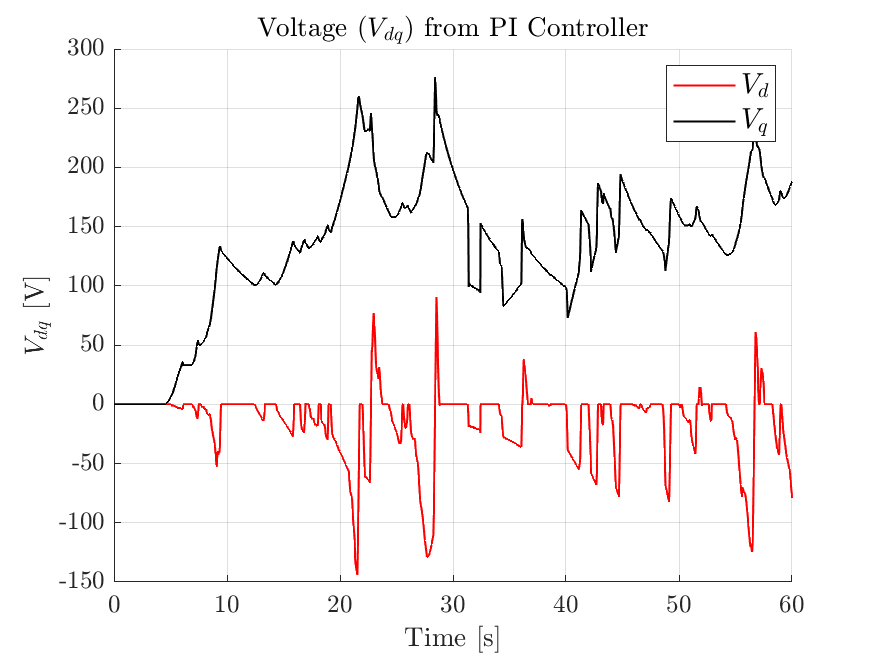
\includegraphics[width=\linewidth]{fig/vdvqPI_plot.png}
        \caption{Voltajes ($V_{d} - V_{q}$).}
    \end{subfigure}
    \caption{Resultados de la simulación.}
    
\end{figure}

Se puede observar que en esta simulación se ha limitado el comportamiento de la frenada regenerativa a la trayectoria del MTPA. Además, se pueden observar ciertos problemas en la implementación del lazo de tensión. Resulta que el control propuesto por \cite{carlos2023} no considera la regeneración, ni mucho menos en debilitamiento de campo. Más adelante se realiza una simulación más enfocada en el control que en la aplicación, y en ella se revisan estas situaciones.

\subsubsection{Modelo conmutado}

Dado que el inversor realmente es una fuente conmutada, se debe modelar utilizando una herramienta que lo permita. Lo único que es necesario discretizar realmente es el control y la generación de tensiones, ya que la planta es continua. Por ello, el primer paso es recalcular las constantes de los lazos de control. Hasta ahora, se habían usado PIs continuos, descritos con la expresión

\begin{equation}
	u(t) = K_p \cdot e(t) + K_i \cdot \int_{0}^{t} e(\tau) d\tau \text{.}
\end{equation}

Cuando se discretiza esta expresión se obtiene

\begin{equation}
	u[k] = K_p \cdot e[k] + K_i \cdot I[k] \text{,}
\end{equation}

donde la integral \( I[k] \) se calcula con una aproximación trapezoidal como

\begin{equation}
	I[k] = I[k-1] + \frac{(e[k] + e[k-1]) \cdot \Delta T}{2} \text{,}
\end{equation}

donde $\Delta T$ es el tiempo de ejecución del PI. Para simplificar el cálculo, se introducen las constantes \( K_0 \) y \( K_1 \), que están relacionadas con \( K_p \) y \( K_i \).

\begin{equation}
	K_0 = K_p + K_i \cdot \frac{\Delta T}{2}
\end{equation}

\begin{equation}
	K_1 = K_i \cdot \frac{\Delta T}{2}
\end{equation}

Así, la ecuación discreta del controlador PI trapezoidal se expresa como

\begin{equation}
	u[k] = u[k-1] + K_0 \cdot e[k] + K_1 \cdot e[k-1] \text{.}
\end{equation}



Utilizando el modelo EMR generado en Simulink se ha implementado la conmutación, pero el tiempo de simulación es demasiado grande como para que sea una herramienta práctica para el desarrollo.

\begin{figure}[H]
    \centering
    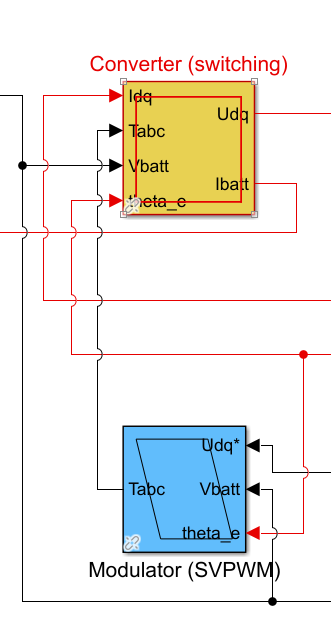
\includegraphics[width=0.25\linewidth]{fig/EMR_VSIsw_out.png}
    \caption{Bloques que contienen el modelo conmutado del VSI con SVPWM.}
    
\end{figure}

\begin{figure}[H]
    \centering

    \begin{subfigure}{0.75\linewidth}
        \centering
        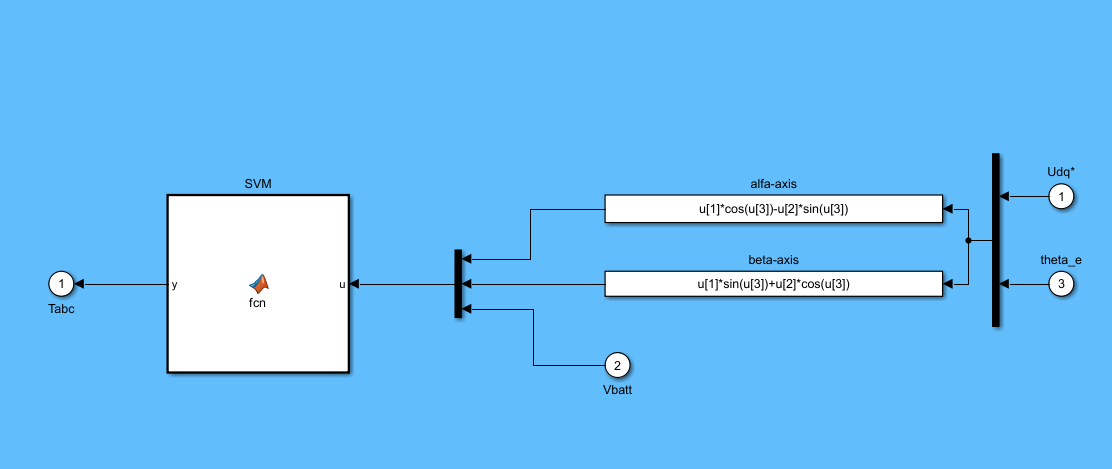
\includegraphics[width=\linewidth]{fig/EMR_VSIsw_in1.png}   
    \end{subfigure}
    \begin{subfigure}{0.75\linewidth}
        \centering
        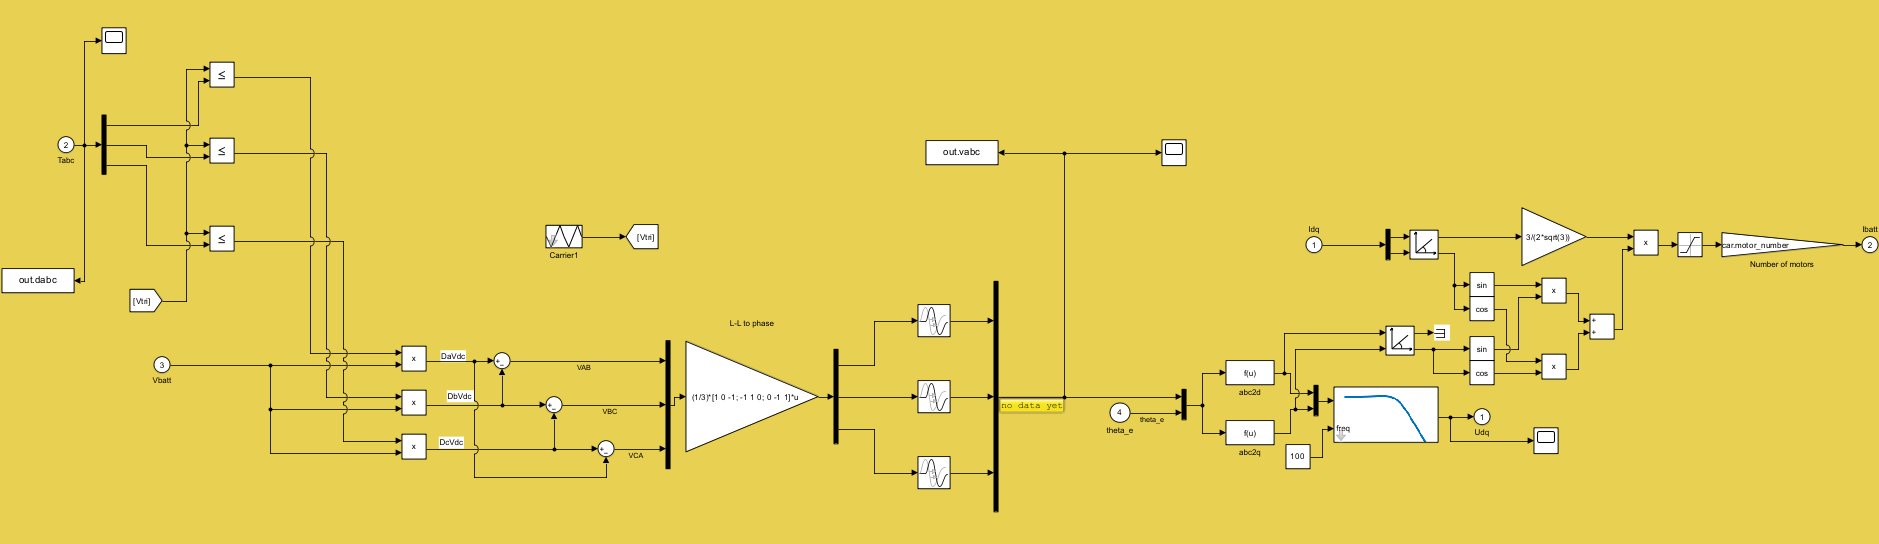
\includegraphics[width=\linewidth]{fig/EMR_VSIsw_in2.png}
    \end{subfigure}
    \caption{Detalle de los bloques del VSI conmutado.}

\end{figure}

\begin{figure}[H]
    \centering
    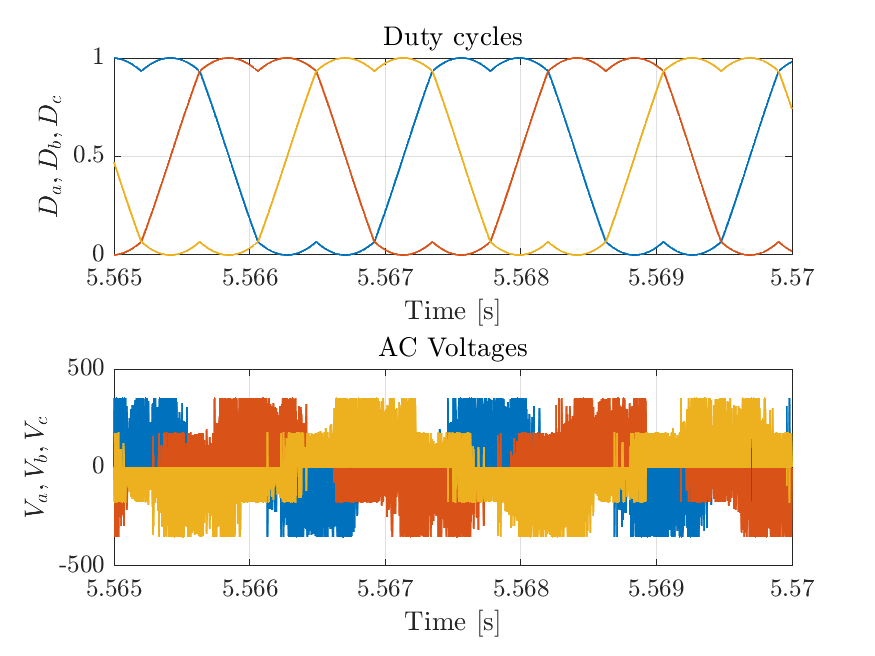
\includegraphics[width=0.85\linewidth]{fig/abc_plot.png}
    \caption{\textit{Duty cycles} y tensiones alternas.}
    
\end{figure}


Por ello se desarrolla un modelo en PLECS que incorpora el lazo de control mejorado, el inversor con MOSFETs, la planta mecánica simplificada, y a la cual se le discretiza la adquisición y el control, de manera que es una aproximación muy realista de la posterior implementación en un microcontrolador. Además se incorporan cálculos térmicos de pérdidas y eficiencia.

\begin{figure}[H]
	\centering
	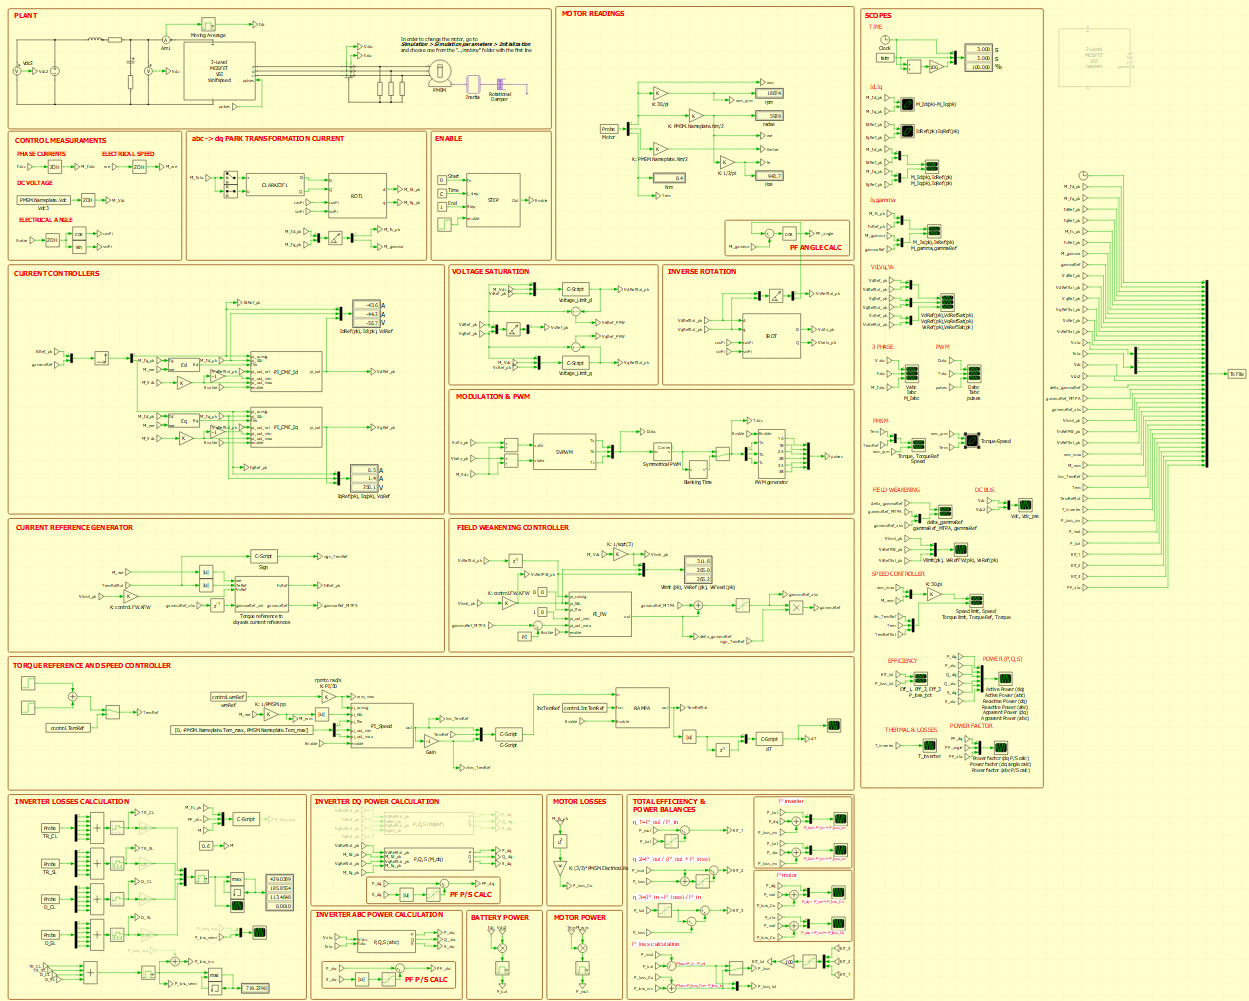
\includegraphics[width=0.7\linewidth]{fig/PLECS_overall}
	\caption{Modelo de simulación en PLECS.}
\end{figure}


Se puede observar que la representación de los bloques en este modelo no sigue el EMR, ya que se elige una implementación más práctica y realista. Destaca la implementación de las funciones de control utilizando la librería PERGAMON, desarrollada por el CITCEA-UPC. Esta librería reproduce completamente el código de las funciones matemáticas implementadas en el control, como los PIs, el SVPWM..., en el \textit{software} PLECS, lo que facilita la correlación de cualquier modelo con la implementación final en un sistema discreto.


A continuación se presentan los diferentes bloques que forman el modelo.
\begin{figure}[H]
	\centering
	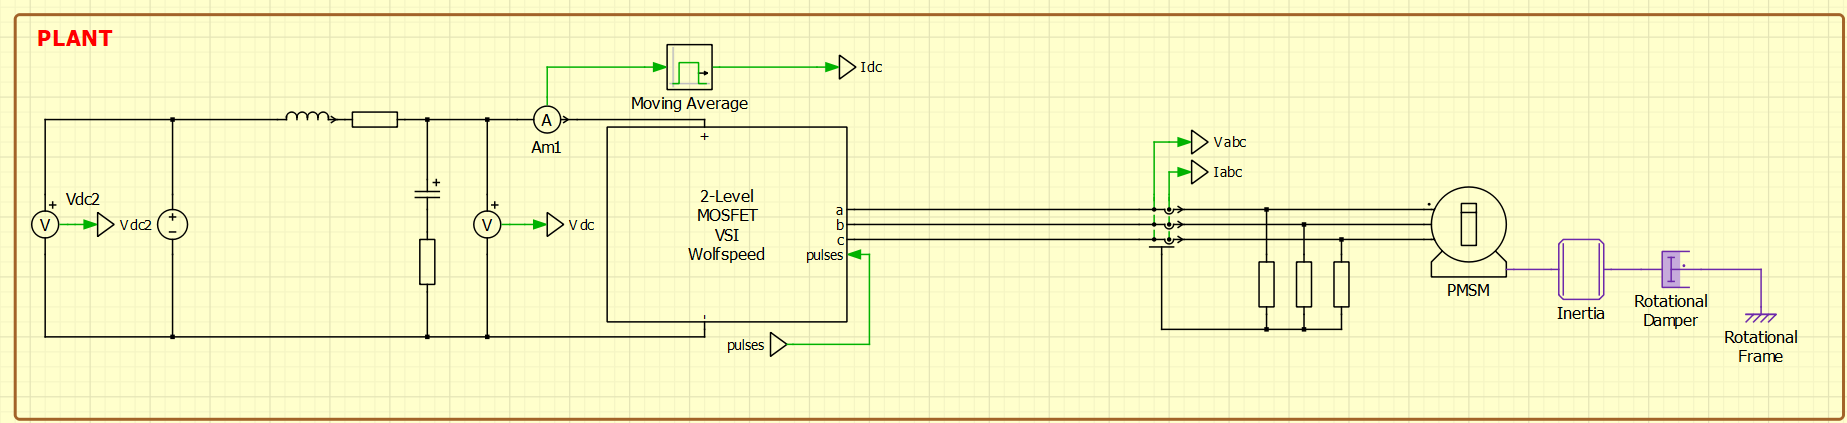
\includegraphics[width=0.7\linewidth]{fig/PLECS_plant}
	\caption{Planta electromecánica del conjunto fuente-inversor-motor-carga.}
\end{figure}

\begin{figure}[H]
	\centering
	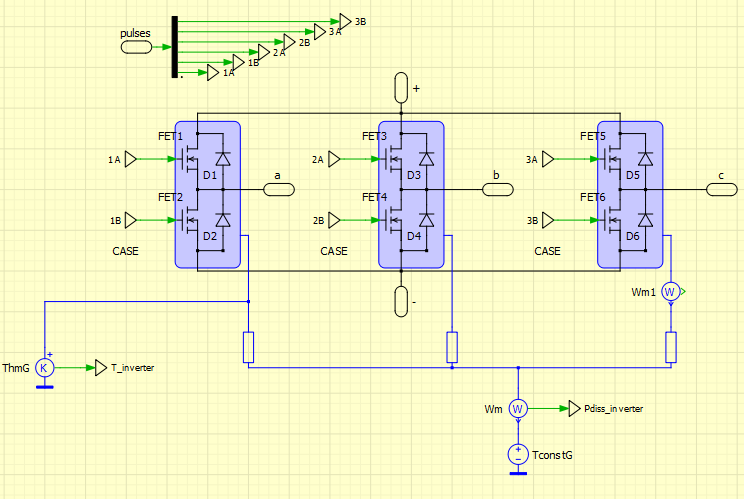
\includegraphics[width=0.7\linewidth]{fig/PLECS_mosfets}
	\caption{Detalle del subbloque VSI, donde se realiza la conexión electrotérmica de los módulos de potencia a la fuente DC, al motor y a la \textit{coldplate}.}
\end{figure}
\begin{figure}[H]
	\centering
	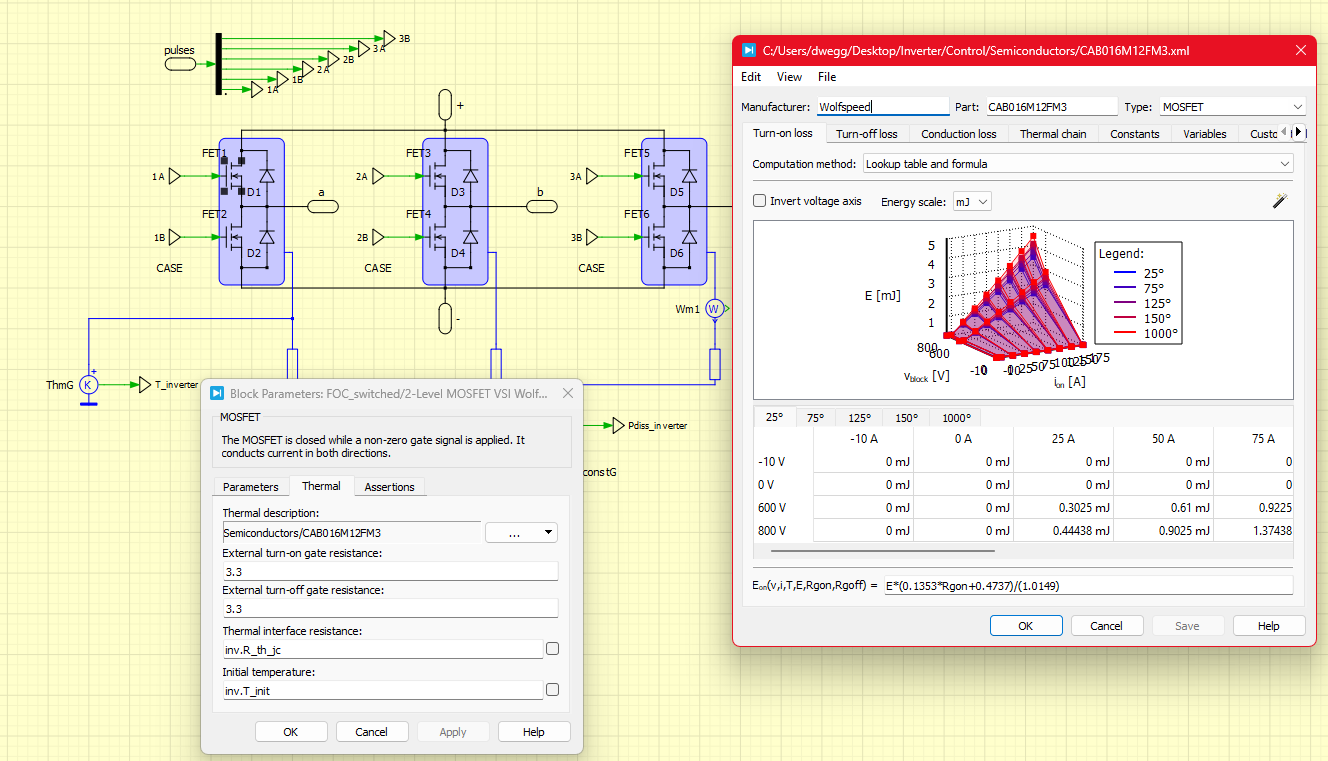
\includegraphics[width=0.7\linewidth]{fig/PLECS_MOSFETs-thermal}
	\caption{Tanto los MOSFETs como los diodos integrados están modelados térmicamente de mano del fabricante, lo que facilita mucho la estimación de pérdidas y la simulación térmica.}
\end{figure}
\begin{figure}[H]
	\centering
	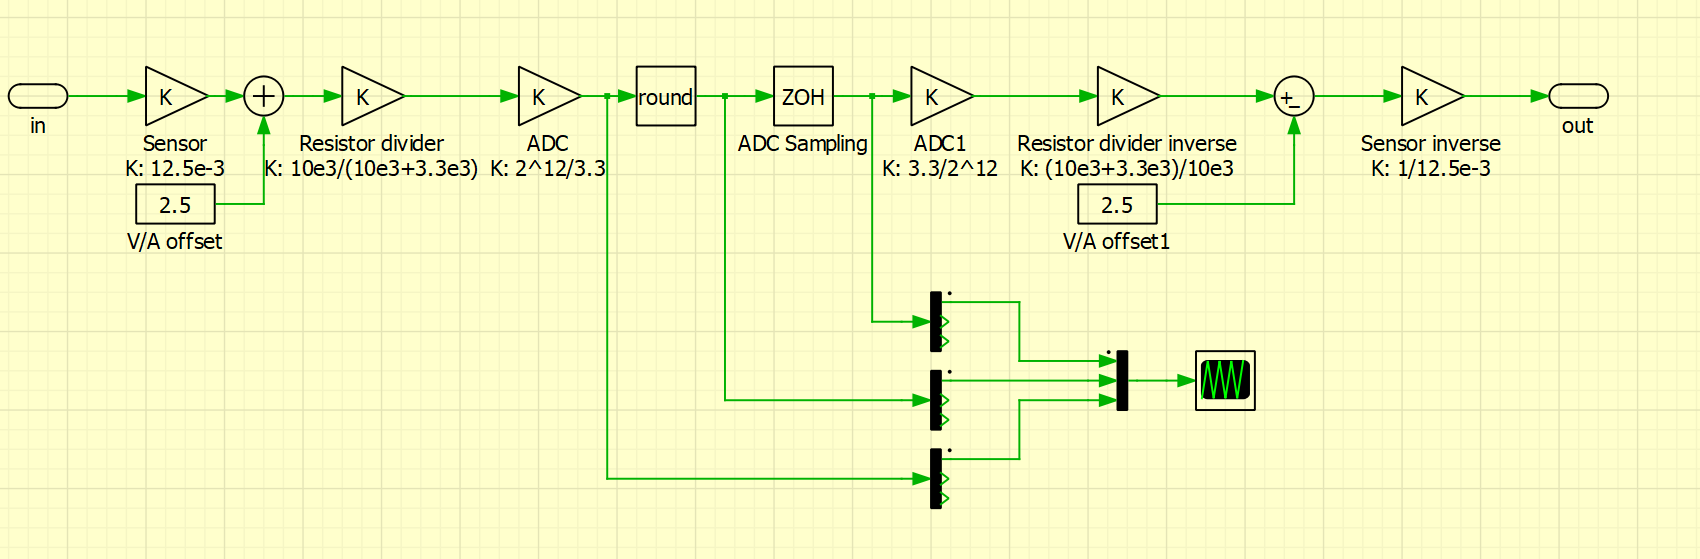
\includegraphics[width=0.7\linewidth]{fig/PLECS_acq}
	\caption{Se modela el ADC mediante el uso de \textit{zero order holds} y cuantizando la adquisición y aplicando las ganancias adecuadas.}
\end{figure}
\begin{figure}[H]
\centering
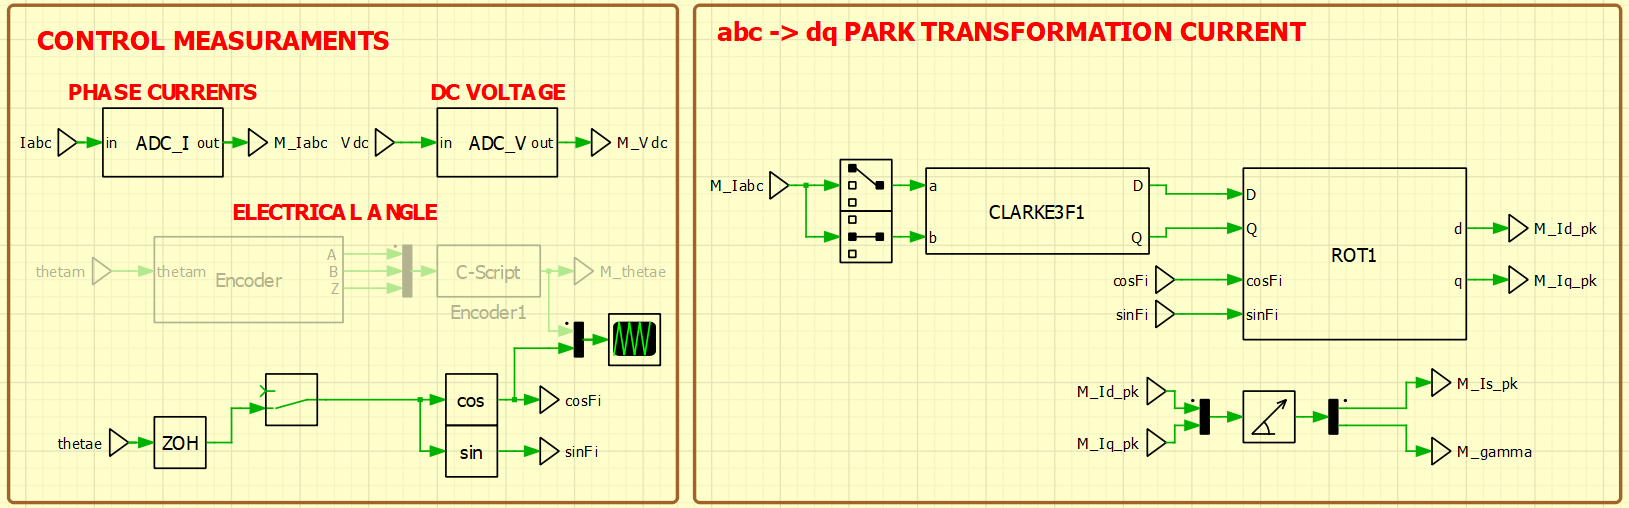
\includegraphics[width=0.7\linewidth]{fig/PLECS_acq2}
\caption{Se implementa la transformada de las corrientes, tanto de $a,b,c$ al espacio $d-q$ como de coordenadas cartesianas a coordenadas polares.}
\end{figure}
\begin{figure}[H]
	\centering
	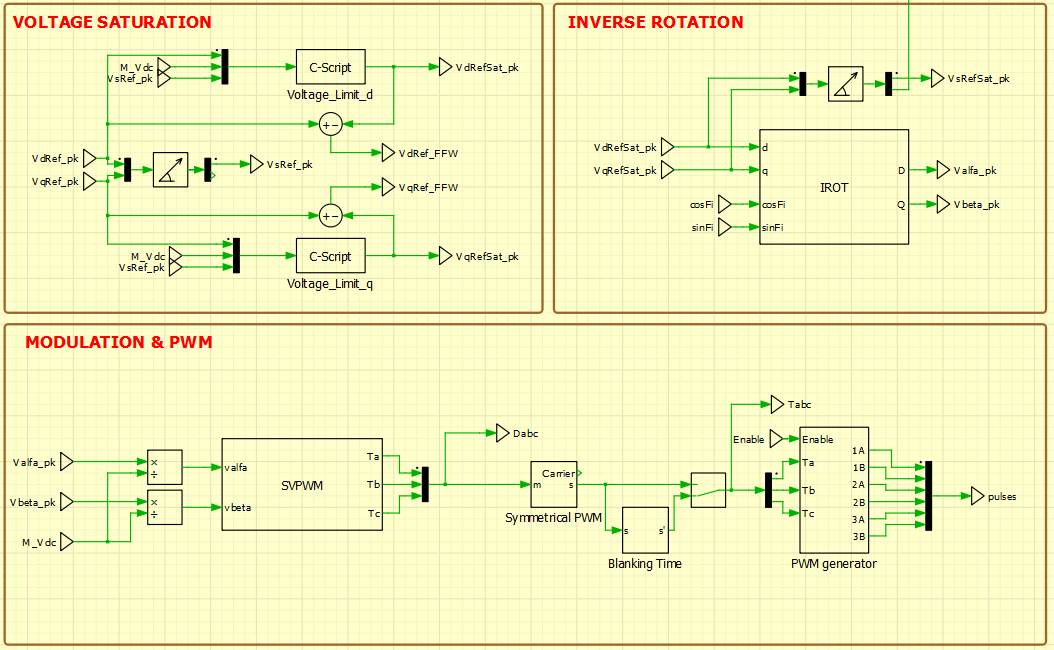
\includegraphics[width=0.7\linewidth]{fig/PLECS_voltage}
	\caption{Saturación y síntesis de las tensiones $V_d$ y $V_q$ mediante la transformada de Clarke inversa y la modulación SVPWM de la librería PERGAMON. Se modelan también los tiempos muertos de la modulación.}
	\label{fig:plecsvoltage}
\end{figure}
\begin{figure}[H]
	\centering
	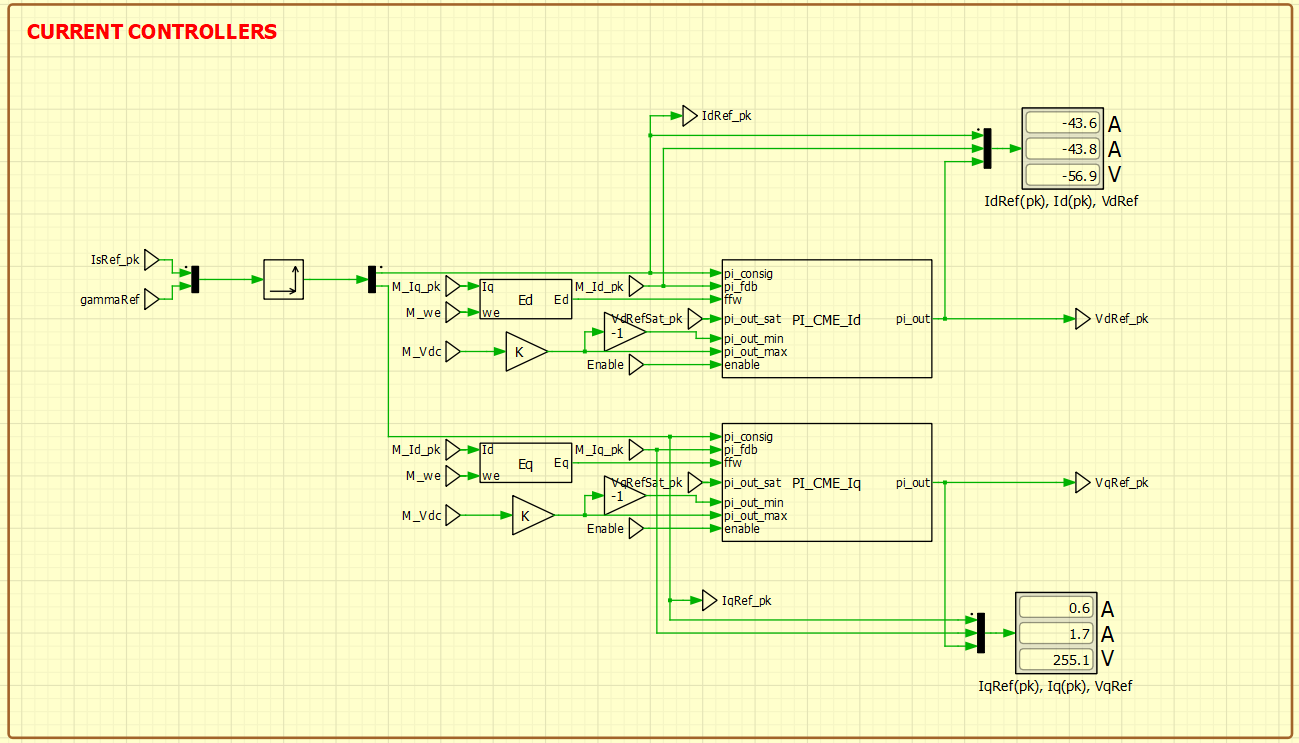
\includegraphics[width=0.7\linewidth]{fig/PLECS_current-loop}
	\caption{Los lazos de corriente están implementados con PIs discretos de la librería PERGAMON y afinados analíticamente con el procedimiento mostrado anteriormente.}
\end{figure}
\begin{figure}[H]
	\centering
	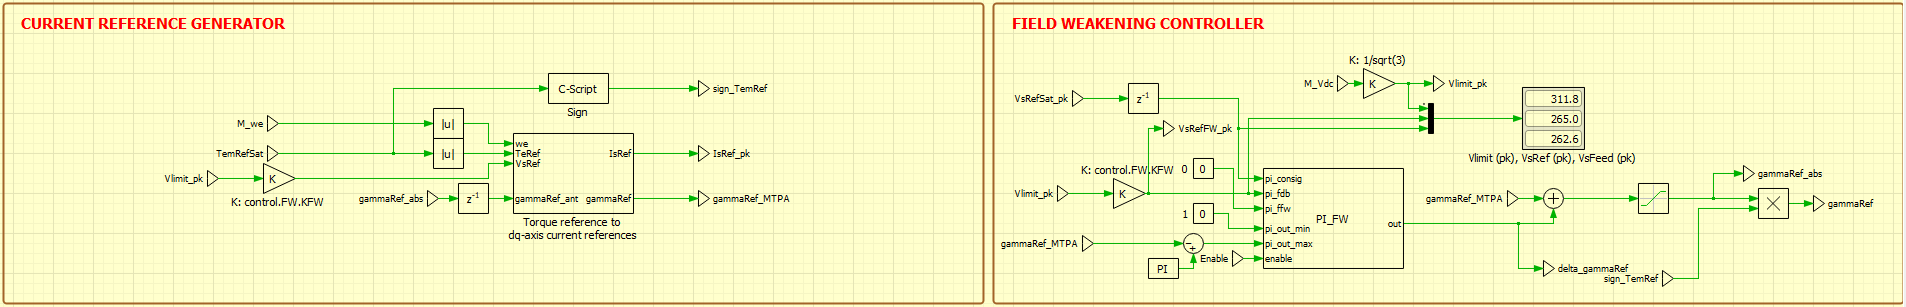
\includegraphics[width=0.9\linewidth]{fig/PLECS_currentref}
	\caption{Consigna de corriente con debilitamiento de campo.}
\end{figure}
\begin{figure}[H]
	\centering
	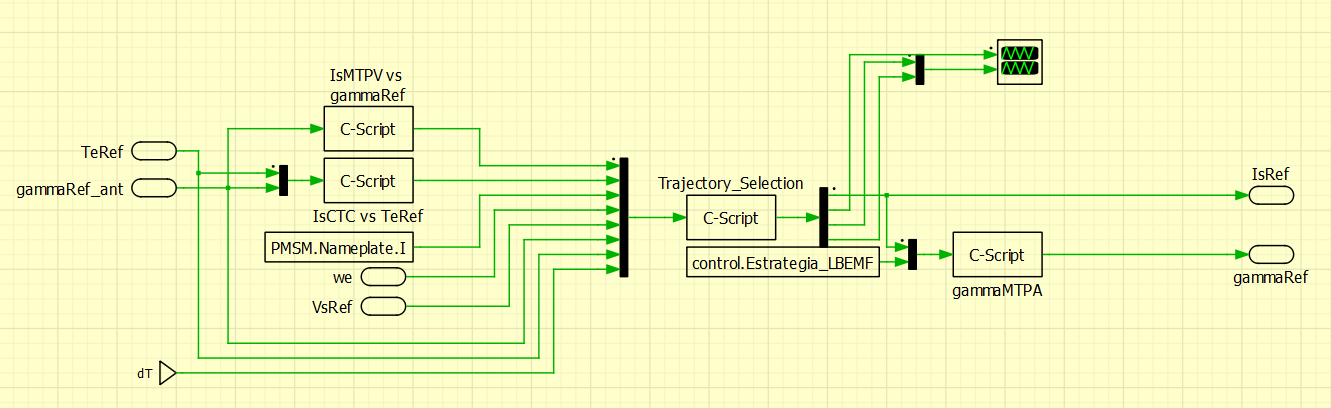
\includegraphics[width=0.7\linewidth]{fig/PLECS_currentref1}
	\caption{Detalle del bloque de cálculo de corriente, donde se implementan las trayectorias de control del PMSM como ecuaciones analíticas resueltas.}
\end{figure}

En esta simulación se ha optado por una estrategia un tanto diferente a la de \cite{carlos2023}. En vez de consignar la corriente mínima de entre todas las trayectorias, se ha implementado una selección más compleja que incorpora la trayectoria VLE y depende de la velocidad eléctrica del motor. Usando esta estrategia más elaborada se consigue un control de la frenada regenerativa más preciso, aunque todavía está en etapa de desarrollo. Hay ciertas situaciones (dependientes de la planta mecánica principalmente) en las que el lazo de tensión no es capaz de ajustar bien el ángulo de corriente y eso lleva a descontroles momentáneos.


\begin{figure}[H]
	\centering
	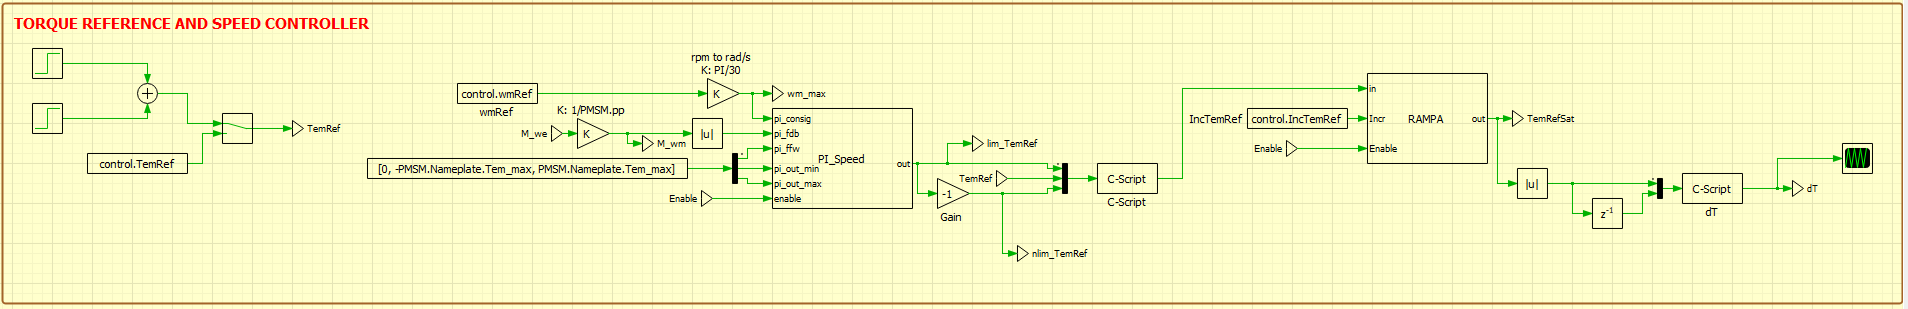
\includegraphics[width=0.9\linewidth]{fig/PLECS_tqspeed}
	\caption{Consigna de par y lazo de velocidad como saturación de la consigna de par.}
\end{figure}
\begin{figure}[H]
	\centering
	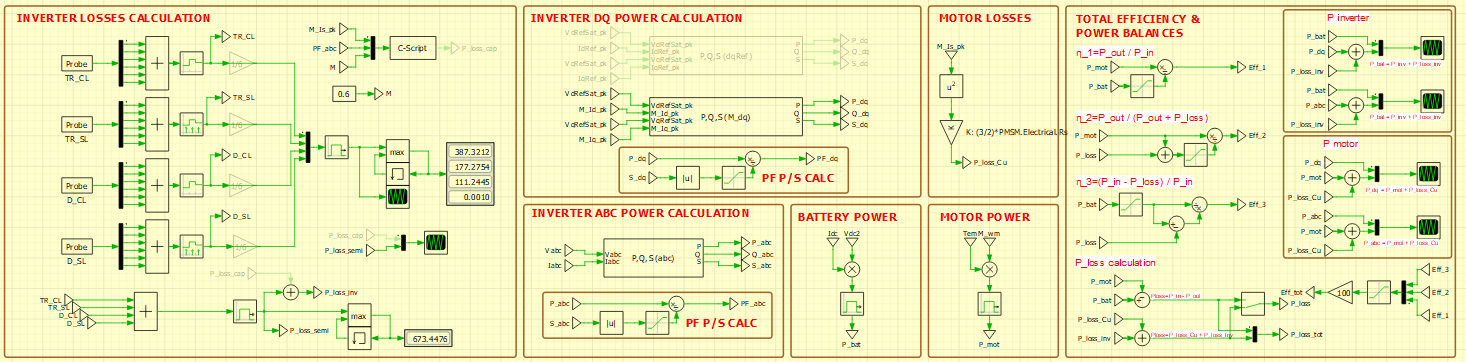
\includegraphics[width=0.7\linewidth]{fig/PLECS_losses}
	\caption{Cálculo de pérdidas, eficiencia y factor de potencia.}
\end{figure}
\begin{figure}[H]
	\centering
	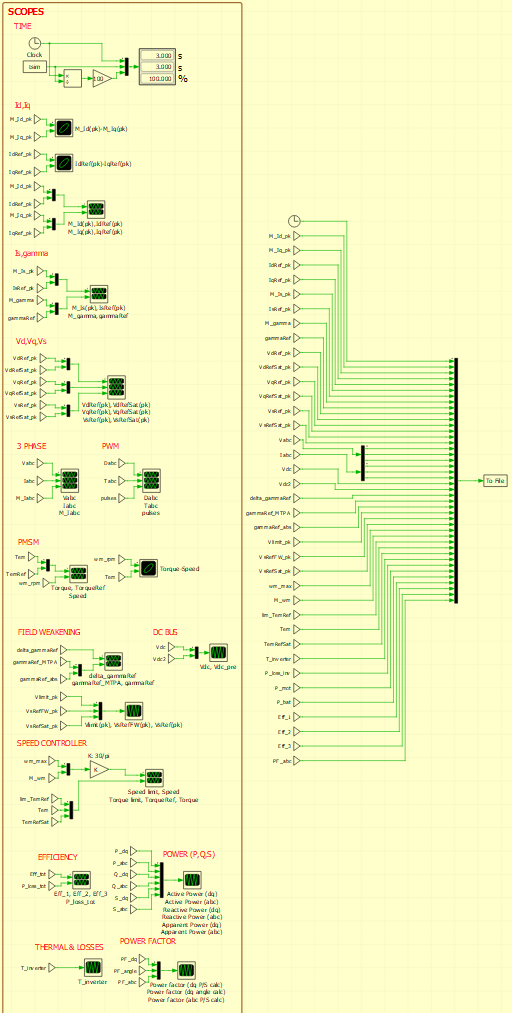
\includegraphics[width=0.4\linewidth]{fig/PLECS_scopes}
	\caption{Visualización y registro de las variables de interés para el análisis y el procesamiento de datos.}
\end{figure}

\begin{figure}[H]
    \centering

    \begin{subfigure}{0.4\textwidth}
        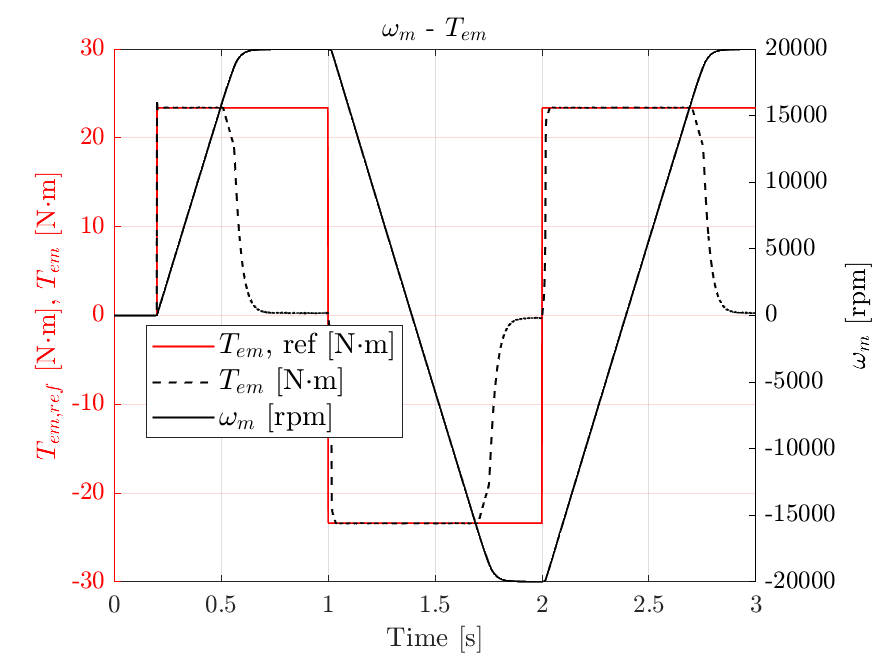
\includegraphics[width=\linewidth]{fig/PLECS_Tem.png}
        \caption{Par electromagnético ($T_{\text{em}}$) y velocidad mecánica ($\omega_{m}$).}
    \end{subfigure}
    %
    \begin{subfigure}{0.4\textwidth}
        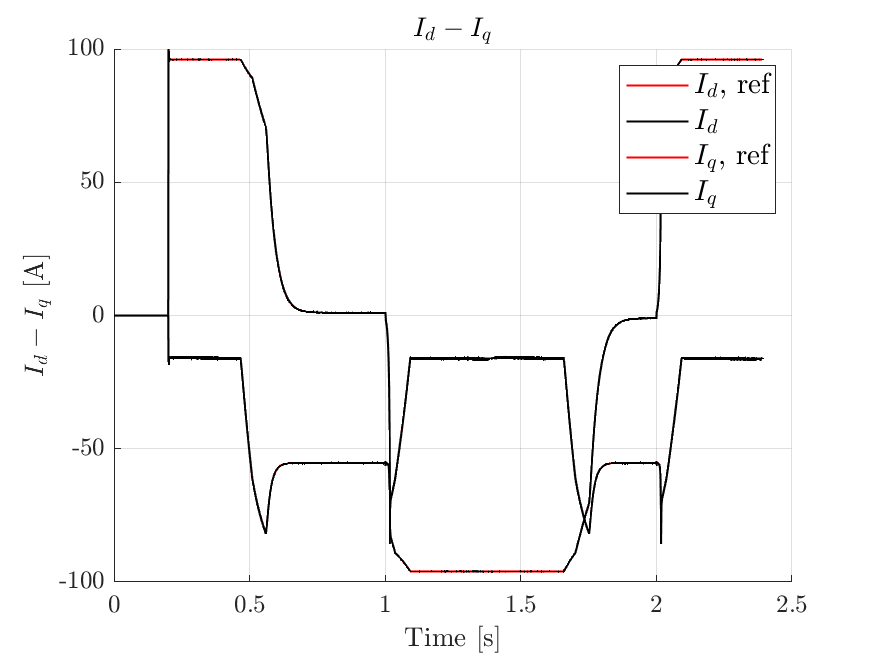
\includegraphics[width=\linewidth]{fig/PLECS_idiq.png}
        \caption{Corrientes ($I_{d} - I_{q}$).}
    \end{subfigure}

    \begin{subfigure}{0.4\textwidth}
        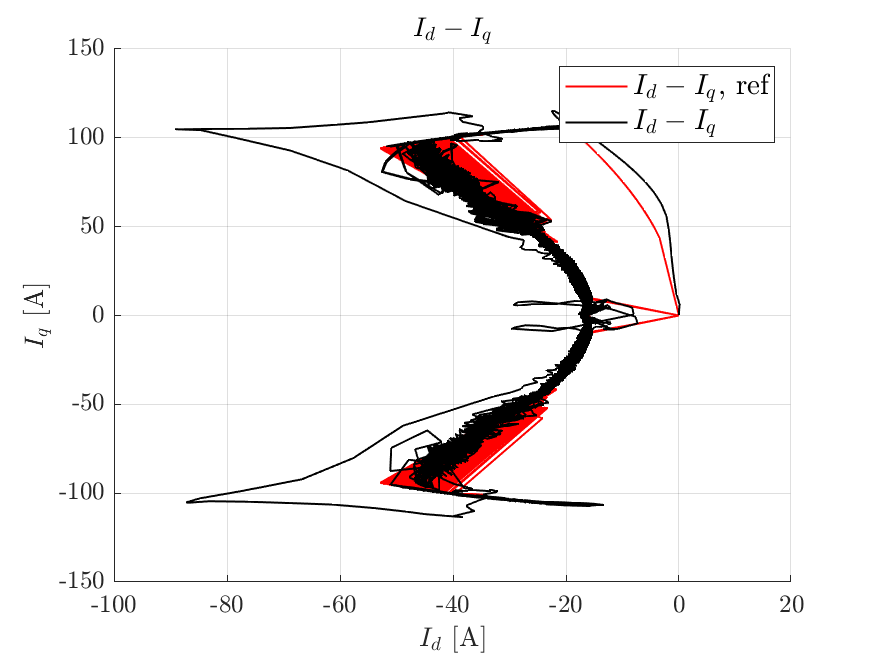
\includegraphics[width=\linewidth]{fig/PLECS_id-iq.png}
        \caption{Corriente ($I_{d}$) vs corriente ($I_{q}$).}
    \end{subfigure}
    %
    \begin{subfigure}{0.4\textwidth}
        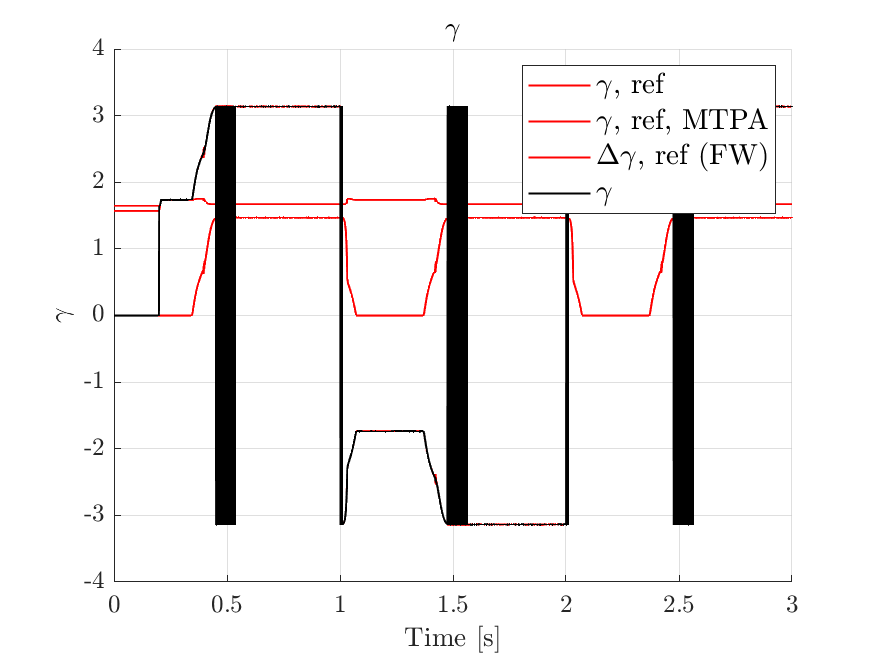
\includegraphics[width=\linewidth]{fig/PLECS_gamma.png}
        \caption{Ángulo de corriente ($\gamma$).}
    \end{subfigure}

    \begin{subfigure}{0.4\textwidth}
        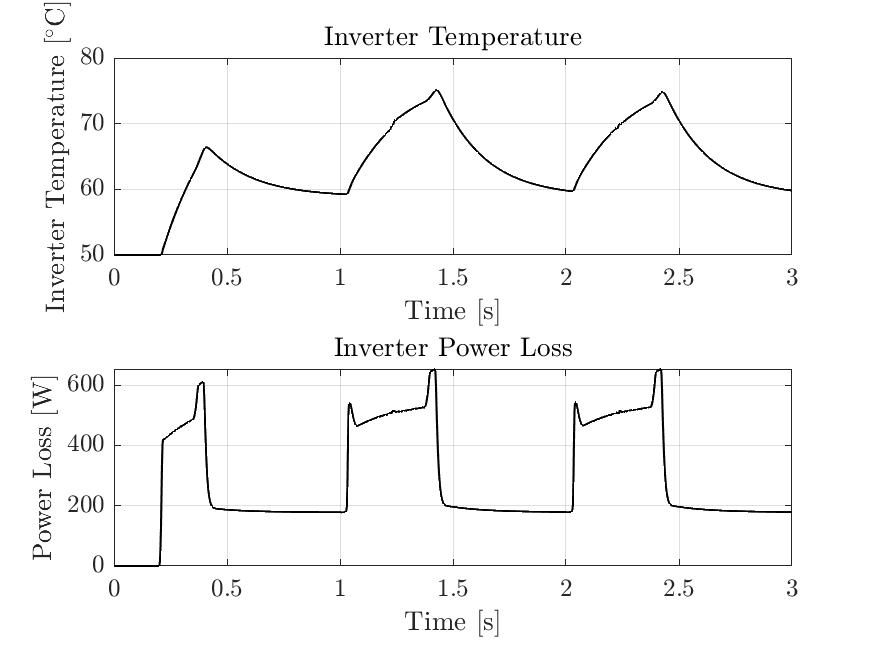
\includegraphics[width=\linewidth]{fig/PLECS_thermal.png}
        \caption{Temperatura y pérdidas del inversor.}
    \end{subfigure}
    %
    \begin{subfigure}{0.4\textwidth}
        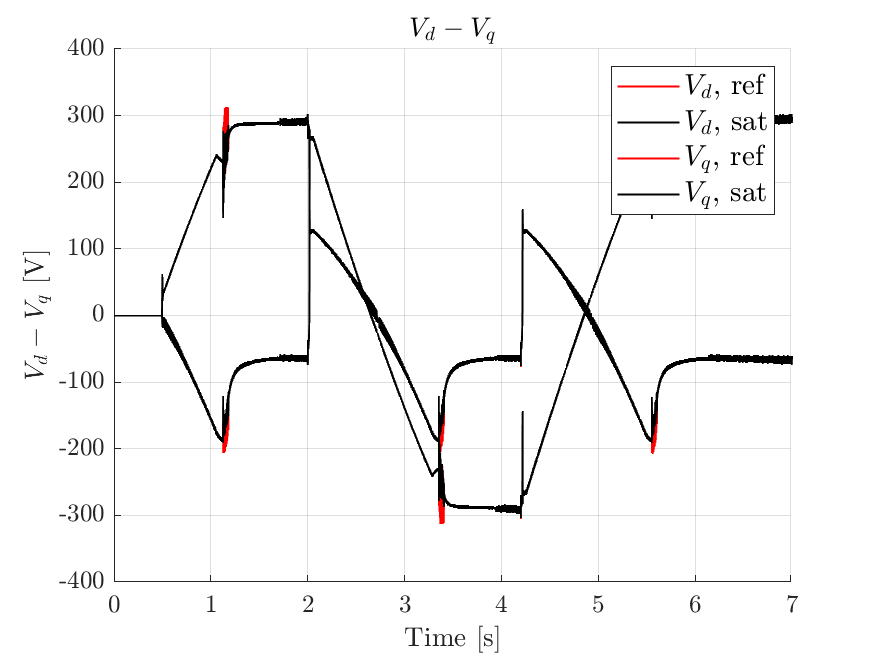
\includegraphics[width=\linewidth]{fig/PLECS_vdvq.png}
        \caption{Voltajes ($V_{d} - V_{q}$).}
    \end{subfigure}

    \caption{Resultados de la simulación.}
\end{figure}

Como se puede observar, se ha optado por consignar un escalón de par del 90\% del par máximo hasta llegar a la velocidad máxima, donde el mismo control es capaz de limitarla. Posteriormente, se consigna un escalón de par igual pero de signo opuesto, para generar una situación extrema y verificar la robustez del control. De esta manera, se evalúa el comportamiento del control vectorial en las circunstancias más adversas, así como el rendimiento teórico del inversor a potencia máxima en los cuatro cuadrantes de operación del motor eléctrico.

Destaca la claridad con la que esta simulación permite apreciar las trayectorias de control en la figura (c), que muestra la consigna y el valor medido de $i_d$ e $i_q$. Como ya se ha comentado, la simulación no refleja un perfil de conducción realista, ya que la frenada regenerativa en debilitamiento de campo no está del todo solucionada para algunas situaciones de carga mecánica.


\newpage
\section{\textit{Hardware}}

\subsection{Requisitos y pre-concepto}

Para definir los requisitos del inversor de tracción, es crucial considerar las restricciones y exigencias del tren de potencia que impone la normativa de la competición \cite{FSG}, así como los parámetros eléctricos del vehículo en particular en el cual se va a implementar.

\subsubsection{Potencia}
La norma \textit{\textbf{EV2.2.1}} \cite{FSG} dicta que la potencia en la salida de la batería no debe exceder los 80 kW. Esta restricción es crucial en el diseño del inversor, ya que se prevé que el vehículo sea impulsado por un solo convertidor con esta potencia máxima. Por ende, el inversor debe estar dimensionado para manejar máximos de potencia de hasta 80 kW. Dado que se trata de un inversor doble, la asignación de potencia se divide en 40 kW por motor, aunque se podría necesitar más potencia en uno de los motores durante la aceleración en una curva. Esta decisión se toma pensando en el futuro del equipo, cuando implemente 4 motores, lo que dotaría al vehículo de hasta 160 kW de máximo. Sin embargo, en ese escenario, solo se podrían utilizar 80 kW repartidos entre las 4 ruedas, con un máximo de 40 kW por rueda.

La prueba donde se espera utilizar esta potencia máxima es la \textit{Acceleration}, donde se podría requerir de los 80 kW durante un máximo de 10 segundos, siendo esta una aproximación muy conservadora. Por lo tanto, la potencia máxima queda como

\colorbox{lightgray}{%
	\parbox{\dimexpr\linewidth-2\fboxsep-2\fboxrule}{%
		\(P_{\text{out, máx, tot}} = 80 \text{ kW} (2 \cdot 40 \text{ kW}) \text{(10 s máx.)}\)
	}%
}



Por otro lado, el requisito de potencia media es distinto. Sería un error dimensionar la potencia media del inversor como el valor máximo, ya que esto conduciría a un sobredimensionamiento excesivo de la refrigeración, los conductores, los conectores y los dispositivos de potencia. En cambio, se opta por determinar el valor medio de potencia requerido durante la prueba más exigente, la \textit{Endurance}. En esta prueba, el vehículo debe recorrer aproximadamente 22 km, lo que equivale a alrededor de media hora de uso continuo. En la \textit{Endurance}, considerar la frenada regenerativa es esencial, ya que aumenta el valor medio de la potencia total, sumándose a la potencia de tracción. Se ha calculado el valor medio de potencia a partir de una simulación de la \textit{Endurance} que llega a máximos de 80 kW.

\begin{figure}[H]
	\centering
	\begin{subfigure}[b]{0.45\textwidth}
		\centering
		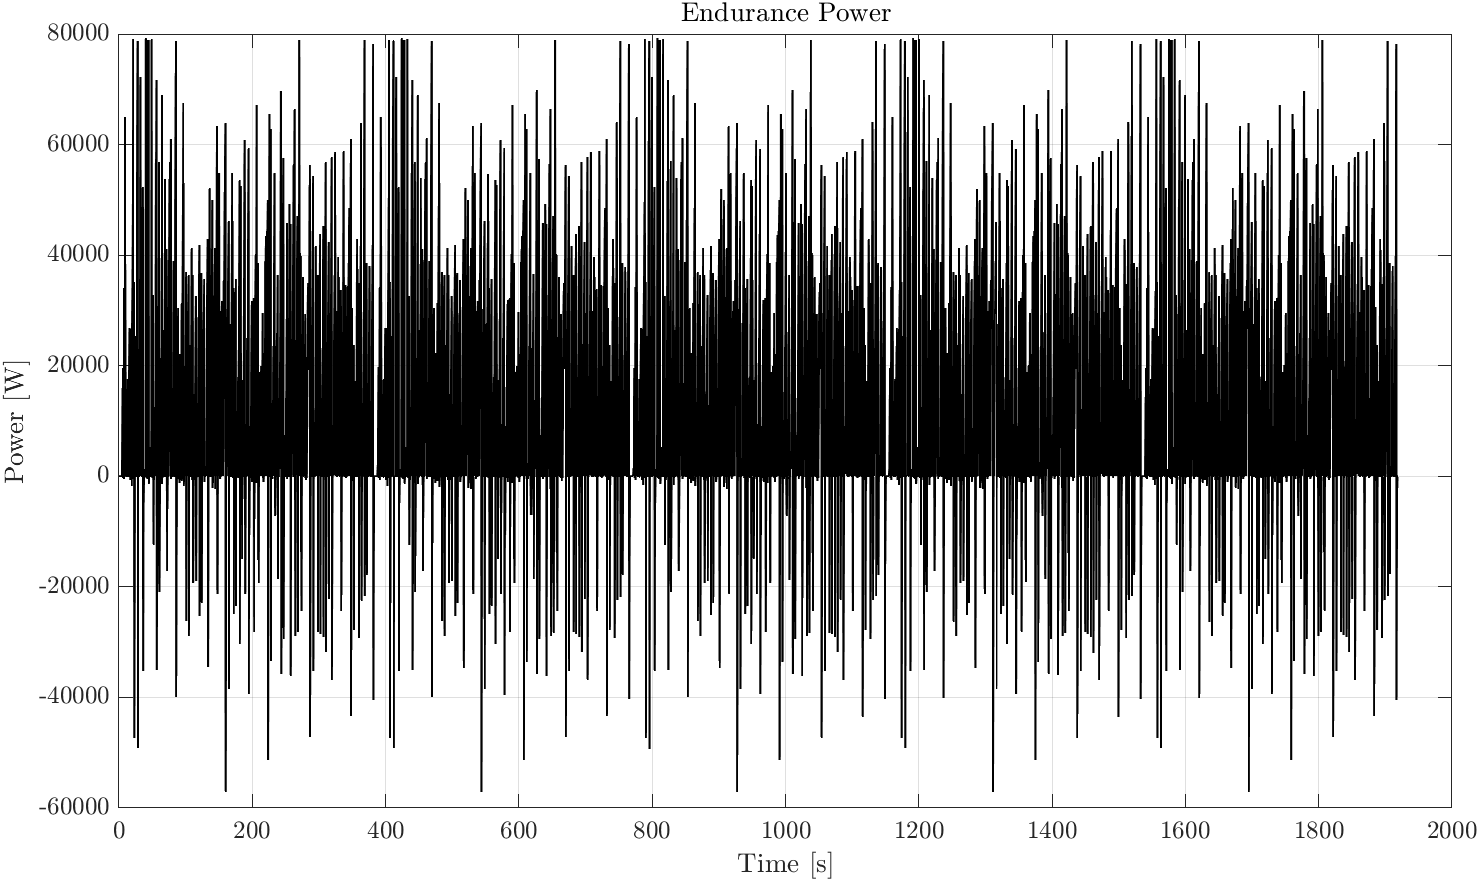
\includegraphics[width=\textwidth]{fig/powerRMS}
	\end{subfigure}
	\hfill
	\begin{subfigure}[b]{0.45\textwidth}
		\centering
		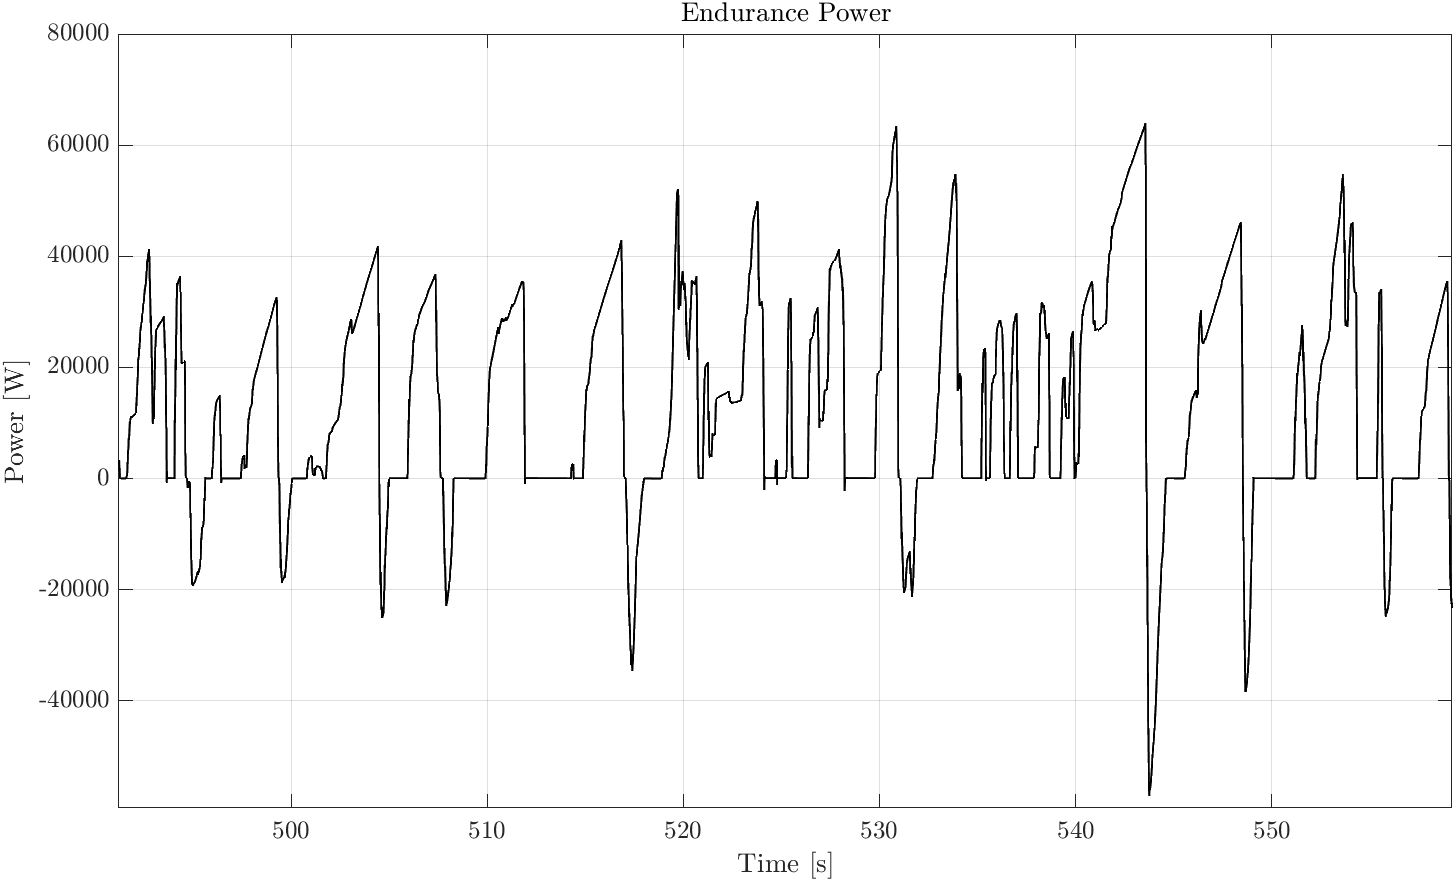
\includegraphics[width=\textwidth]{fig/powerRMS-zoom}
	\end{subfigure}
	\caption{Potencia instantánea que sale de la batería en un evento de \textit{Endurance} (Tiempo completo y detalle de un fragmento).}
\end{figure}

A continuación se muestra el cálculo del valor RMS de la potencia requerida, basado en los datos de potencia:

\begin{verbatim}
	% Calcular el cuadrado de los valores de potencia
	power_squared = power_time.Data.^2;
	
	% Calcular el promedio de los valores cuadrados
	mean_power_squared = mean(power_squared);
	
	% Tomar la raíz cuadrada del promedio de los valores cuadrados para obtener 
	% el valor RMS
	power_rms = sqrt(mean_power_squared);
	
	power_rms =
	
	2.3193e+04
\end{verbatim}


Esto demuestra que el valor medio de potencia requerido es considerablemente menor que el pico máximo, en concreto un \(\frac{23.2 \text{ kW}}{80 \text{ kW}} = 29\%\). Por lo tanto, se dimensiona el inversor considerando una potencia media de 35 kW, es decir, 17,5 kW por motor. Esta cifra proporciona un margen de seguridad de 11,8 kW respecto a la simulación, lo que permite algo de juego en el reparto de potencia entre ambos motores. De esta manera, la potencia constante queda como

\colorbox{lightgray}{%
	\parbox{\dimexpr\linewidth-2\fboxsep-2\fboxrule}{%
		\(P_{\text{out, const, tot}} = 35 \text{ kW} (2 \cdot 17.5 \text{ kW})\)
	}%
}

Cabe destacar que se está calculando la potencia aparente del convertidor, ya que la potencia activa y la reactiva se reparten en función del factor de potencia, que no es constante y depende de la planta mecánica y la situación del motor. La potencia activa es la que usa el motor para acelerar o frenar, y la reactiva la consume o suministra el bus de condensadores. Otra nota es que la simulación es poco realista puesto que utiliza picos de potencia máxima, cuando en realidad, en la prueba de la \textit{Endurance} se suele limitar el valor de estos picos con tal de extender la autonomía.

Además, existe la norma \textit{\textbf{EV4.1.1} The maximum permitted voltage that may occur between any two electrical connections is 600 V,DC and for motor controller/inverters internal low power control signals 630 V,DC.}, que impone el límite de 600 V para la tensión de bus máxima. Es de interés que el inversor esté dimensionado a esta tensión de funcionamiento, \textbf{600 V,DC}, para permitir máxima flexibilidad con el diseño de la batería, por ejemplo. Al usar la tensión más alta posible, se obtiene un beneficio en la reducción de la corriente, que implica menos pérdidas en los conductores y permite reducir la sección de cables, pletinas, conectores y otros conductores.

Ya que la estrategia de modulación es SVPWM y la tensión máxima es de 600 V, la tensión alterna fase-neutro de un motor se expresa como

\(V_{\text{fase-neutro, pico, 600 V,DC}} = \frac{V_{\text{DC}}}{\sqrt{3}} = \frac{600 \text{ V}}{\sqrt{3}} = 346 \text{ V}\)

\(V_{\text{fase-neutro, RMS, 600 V,DC}} = \frac{V_{\text{fase-neutro, pico}}}{\sqrt{2}} = \frac{346 \text{ V}}{\sqrt{2}} = 245 \text{ V}\)

Sin embargo, la batería no estará constantemente a 600 V,DC, por lo que para poder entregar la potencia de 40 kW pico por inversor en un rango de tensiones adecuado se debería calcular la corriente con una tensión menor. Se escoge 450 V,DC como tensión mínima a partir de la cual se puede entregar la potencia máxima de 40 kW por inversor. Entonces, la corriente de fase de un motor queda

\(V_{\text{fase-neutro, pico, 450 V,DC}} = \frac{V_{\text{DC}}}{\sqrt{3}} = \frac{450 \text{ V}}{\sqrt{3}} = 261 \text{ V}\)

\(V_{\text{fase-neutro, RMS, 450 V,DC}} = \frac{V_{\text{fase-neutro, pico}}}{\sqrt{2}} = \frac{261 \text{ V}}{\sqrt{2}} = 184 \text{ V}\)


\(I_{\text{fase, RMS, máx}} = \frac{P_{\text{out, máx}}}{3\cdot V_{\text{fase-neutro, RMS, 450 V,DC}}} = \frac{40 \text{ kW}}{3\cdot184 \text{ V}} = 72 \text{ A}\)

\(I_{\text{fase, pico, máx}} = I_{\text{fase, RMS, máx}}\cdot\sqrt{2} = 72\text{A} \cdot\sqrt{2} = 102 \text{ A}\)

De la misma manera que con la potencia, se puede obtener el valor de corriente constante a una tensión menor, ya que el resultado será más restrictivo.

\(I_{\text{fase, RMS, const}} = \frac{P_{\text{out, const}}}{3\cdot V_{\text{fase-neutro, RMS, 450 V,DC}}} = \frac{17.5 \text{ kW}}{3\cdot184 \text{ V}} = 32 \text{ A}\)

\(I_{\text{fase, pico, const}} = I_{\text{fase, RMS, const}}\cdot\sqrt{2} = 32 \text{ A}\cdot\sqrt{2} = 45 \text{ A}\)


Iterando el cálculo de potencia, se puede ver que si se dimensiona a estas corrientes, las potencias máxima y constante calculadas a 600 V,DC son considerablemente mayores.

\(P_{\text{out, máx}} = 3\cdot V_{\text{fase-neutro, RMS, 600 V,DC}}\cdot I_{\text{fase, RMS, máx}} = 3\cdot245 \text{ V}\cdot 72 \text{ A} = 53 \text{ kW}\)

\(P_{\text{out, const}} = 3\cdot V_{\text{fase-neutro, RMS, 600 V,DC}}\cdot I_{\text{fase, RMS, const}} = 3\cdot245 \text{ V}\cdot 32 \text{ A} = 23.5 \text{ kW}\)

\(P_{\text{out, máx, tot}} = 2\cdot P_{\text{out, máx}} = 2\cdot53 \text{ kW} = 106 \text{ kW}\)

\(P_{\text{out, const, tot}} = 2\cdot P_{\text{out, const}} = 2\cdot23.5 \text{ kW} = 47 \text{ kW}\)


\subsubsection{Velocidad}
Puesto que se va a controlar un motor con posibilidad de operación en debilitamiento de campo, es necesario conocer la frecuencia eléctrica máxima que se va a tener que poder sintetizar. Este requisito va a dimensionar la velocidad de los lazos de control, y en última instancia, la frecuencia de conmutación. El motor en estudio tiene 3 pares de polos y una velocidad angular mecánica máxima de 20000 RPM. Por lo tanto, la frecuencia eléctrica máxima que se debe sintetizar se calcula

\(f_{\text{e,máx}} = \frac{pp\cdot \omega_{\text{m, máx, RPM}}}{60} = \frac{3\cdot 20000}{60} = 1000 \text{ Hz .}\)

Dejando un poco de margen para la compatibilidad con motores de más polos, se escoge una frecuencia máxima de 1200 Hz. Para sintetizar esta frecuencia eléctrica con poca distorsión armónica, se debe escoger una frecuencia de conmutación al menos 30 veces superior, para tener como mínimo 30 pulsos por periodo a estas frecuencias.


\colorbox{lightgray}{%
	\parbox{\dimexpr\linewidth-2\fboxsep-2\fboxrule}{%
		\(f_{\text{conm}} > 30\cdot f_{\text{e,máx}} = 30\cdot1200 \text{ Hz} = 36 \text{ kHz} \rightarrow f_{\text{conm}} = 40 \text{ kHz}\)
	}%
}

Se debe considerar también que con una frecuencia de conmutación mayor, las pérdidas de conmutación serán más grandes, pero el tamaño del bus de condensadores será más pequeño. Además, el lazo de control debe ir a 40 kHz, con lo que el microcontrolador que lo implemente debe ser capaz de ejecutar todos los cálculos en menos de $\frac{1}{40 \text{ kHz}} = 25 \text{ }\text{\unit{\micro\second}}$.

Es importante que el control sea mucho más rápido que la planta eléctrica, cuya constante de tiempo es de

\(\text{min}(\frac{L_d}{R_s},\frac{L_q}{R_s}) = \text{min}(\frac{188.7 \text{ }\text{\unit{\micro\henry}}}{0.15 \text{ }\Omega},\frac{283.1 \text{ }\text{\unit{\micro\henry}}}{0.15 \text{ }\Omega}) = \text{min}(1.258 \text{ ms}, 1.887 \text{ ms}) = 1.258 \text{ ms}\)

\(1.258 \text{ ms} >> 25 \text{ }\text{\unit{\micro\second} .}\)

\subsubsection{Normativa}
La normativa de la Formula Student no impone normativas muy restrictivas, ya que la mayoría están enfocadas a la seguridad. Estas son las normas que afectarán al diseño del inversor:

\begin{itemize}

    \item \textit{\textbf{EV2.2.2} Regenerating energy is allowed and unrestricted.} La posibilidad de regenerar energía implica que el inversor debe ser capaz de consignar par en el sentido opuesto a la velocidad de los motores para frenar, lo que tendrá un impacto fundamental en el diseño del control. La topología de VSI es bidireccional en sí misma.
    \item \textit{\textbf{EV2.2.3} Wheels must not be spun in reverse.} Podría impactar la lógica de control del inversor y en la adquisición de los sensores de posición para evitar la marcha atrás. Se pueden implementar algoritmos de dependencia de dirección para que ambos motores traccionen el vehículo en la misma dirección.
    \item \begin{itquote} \textbf{EV3.1.1} TS enclosures, see EV1.1.2, must consist of either
    \begin{itemize}
            \item a grounded solid layer made of at least 0.5 mm thick electrically conductive material, aluminium or better, having a resistance below 300 m$\Omega$, measured with a current of 1 A, to LVS ground and able to continuously carry at least 10\% of the TS accumulator main fuse current rating or 
            \item be fully made out of electrically insulating materials having an isolation resistance of at least 2 M$\Omega$, measured with a voltage of 500 V. The enclosure must be rigid and must prevent possible mechanical penetrations. Protruding electrically conductive parts, such as fasteners or connectors, must follow EV3.1.2
    \end{itemize} The TSAC might use at least 0.9 mm thick steel layer as the grounded layer. \end{itquote} Tendrá efectos en el diseño del empaquetado del convertidor y en la selección de materiales para garantizar la seguridad eléctrica y mecánica del convertidor.

    \item \textit{\textbf{EV3.2.5} All overcurrent protection devices that are part of the TS must not rely on programmable logic. The overcurrent protection function of motor controllers/inverters for the motor outputs may rely on programmable logic.} Los dispositivos de protección contra sobrecorriente en el sistema de tracción para el motor pueden depender de lógica programable, lo que permite utilizar el sensado de corriente para garantizar esta protección.
    \item \textit{\textbf{EV4.1.2} All components in the TS must be rated for the maximum TS voltage. The TS area of a PCB, see EV4.3.6, is considered as one component. Every input connected to the TS must be rated to the maximum TS voltage.} Tendrá efectos en la selección de los componentes del circuito de potencia del inversor.
    \item \textit{\textbf{EV4.1.3}  All components must be rated for the maximum possible temperature that may occur during usage.} Impactará en la selección de componentes que puedan manejar las temperaturas esperadas.
    \item \textit{\textbf{EV4.2.1} TS enclosures, see EV1.1.2, must be labeled with (a) reasonably sized sticker(s) according to “ISO 7010-W012” (triangle with a black lightning bolt on a yellow background). The sticker must also contain the text “High Voltage” if the voltage is more than 60 V,DC or 50 VACRMS.} Impacta en los requisitos de señalización y seguridad del empaquetado.
    \item \textit{\textbf{EV4.3.1} The entire TS and LVS must be galvanically isolated, see EV1.2.1 and IN4.1.1.} Afecta el diseño de la separación y el aislamiento entre ambos sistemas.
    \item \textit{\textbf{EV4.3.4} Where both TS and LVS are present within an enclosure, they must be separated by barriers made of moisture-resistant insulating materials or maintain the following spacing through the air, or over a surface:}

	\begin{table}[H]
		\centering
		\caption{Voltage Spacing Requirements}
		\begin{tabular}{|l|l|}
			\hline
			Voltage         & Spacing     \\ \hline
			\(U < 100 \text{V,DC}\)  & 10 mm       \\ \hline
			\(100 \text{V,DC} < U < 200 \text{V,DC}\) & 20 mm       \\ \hline
			\(U > 200 \text{V,DC}\)  & 30 mm       \\ \hline
		\end{tabular}
	\end{table} Impacta en el diseño del empaquetado del inversor.  Se usarán aislantes como el Nomex en caso de que no se pueda garantizar el espaciado por aire.
    \item \textit{\textbf{EV4.3.6} If TS and LVS are on the same PCB, they must be on separate well-defined areas of the board, meeting the spacing requirements in table 5, each area clearly marked with “TS” or “LV”. The outline of the area required for spacing must  be marked. “Conformal coating” refers to a coating insulator, solder resist is not a coating.}
    
	\begin{table}[H]
		\centering
		\caption{Voltage Spacing Requirements}
		\begin{tabular}{|l|l|l|l|}
			\hline
			Voltage & Over Surface & Through Air (Cut in board) & Conformal Coating \\
			\hline
			0 to 50 & 1.6 mm & 1.6 mm & 1.0 mm \\
			\hline
			50 to 150 & 6.4 mm & 3.2 mm & 2.0 mm \\
			\hline
			150 to 300 & 9.5 mm & 6.4 mm & 3.0 mm \\
			\hline
			300 to 600 & 12.7 mm & 9.5 mm & 4.0 mm \\
			\hline
		\end{tabular}
	\end{table} Tendrá efectos en el diseño de la PCB de potencia.

    \item \textit{\textbf{EV4.5.3} The temperature rating for TS wiring, connections, and insulation must be appropriate for the expected surrounding temperatures but at least 85 $\si{\degreeCelsius}$.} Influirá en la selección de cables y materiales aislantes.
    \item \textit{\textbf{EV4.5.4} TS components and containers must be protected from moisture in the form of rain or puddles, see IN9.} Impactará en el diseño de la caja.
    \item \textit{\textbf{EV4.5.6} All TS wiring must be completed to professional standards with appropriately sized conductors and terminals and with adequate strain relief and protection from loosening due to vibration etc.} Tendrá efectos en el diseño de las conexiones y terminales.
    \item \textit{\textbf{EV4.5.10} Every TS connector outside of a housing must include a pilot contact/interlock line which is part of the SDC. Housings only used to avoid interlocks are prohibited.} Impactará en el diseño de los conectores y sistemas de interconexión.
    \item \textit{\textbf{EV4.5.11} All TS connections must be designed so that they use intentional current paths through conductors such as copper or aluminium and must not rely on steel bolts to be the primary conductor.} Tendrá efectos en el diseño de las conexiones y la selección de materiales adecuados.
    \item \textit{\textbf{EV4.5.12} All TS connections must not include compressible material such as plastic in the stack-up or as a fastener. FR-4 is allowed.} Impactará en el diseño de las conexiones y la selección de materiales adecuados.
    \item \textit{\textbf{EV4.5.13} TS connectors outside of TS enclosures must be designed in a way, that the TS cannot be activated, see EV4.11, if connected in any way other than the design intent configuration.} Tendrá efectos en el diseño de los conectores y la seguridad.
    \item \textit{\textbf{EV4.5.14} All electrical connections, including bolts, nuts, and other fasteners, in the high current path of the TS must be secured from unintentional loosening. Fasteners must use positive locking mechanisms, see T10.2, that are suitable  for high temperatures, see EV4.5.3.} Impactará en el diseño de los sistemas de fijación y bloqueo, especialmente en las conexiones de potencia.
    \item \begin{itquote} \textbf{EV4.5.16} Soldered connections in the high current path are only allowed if all of the following are true: 
    \begin{itemize}
            \item connections on PCBs
            \item the connected devices are not cells or wires
            \item the devices are additionally mechanically secured against loosening
    \end{itemize} \end{itquote} Tendrá efectos en el diseño de las conexiones y el uso de soldaduras. El uso de sistemas alternativos de conexión en placa como el \textit{press-fit}, facilita el cumplimiento de esta norma.
    \item \textit{\textbf{EV4.9.1} If a discharge circuit is required to meet EV6.1.5, it must be designed to handle the maximum TS voltage permanently. After three subsequent discharges within 15 s in total, the discharge time specified in EV6.1.5 may be exceeded.  Full discharging functionality must be given after a reasonable time with a deactivated discharge circuit.} Se deberá integrar un circuito de descarga en el inversor que cumpla con estos requisitos.
    \item \textit{\textbf{EV4.9.2} The discharge circuit must be wired in a way that it is always active whenever the SDC is open. Furthermore, the discharge circuit must be fail-safe such that it still discharges the intermediate circuit capacitors if the HVD has  been opened or the TS accumulator is disconnected.} Tendrá efectos en la implementación del circuito de descarga.
    \item \begin{itquote} \textbf{EV2.2.1} EV4.10.2 The TSAL itself must have a red light, flashing continuously with a frequency between 2 Hz and 5 Hz and a duty cycle of 50\%, active if and only if the LVS is active and the voltage across any DC-link capacitor exceeds 
    \begin{itemize}
            \item 60 V,DC or 50 VACRMS
            \item Half the nominal TS voltage
    \end{itemize} 
    whichever is lower \end{itquote} Se deberá implementar esta detección.
    \item \textit{\textbf{EV4.10.4} The mentioned voltage detection must be performed inside the respective TS enclosure.} Obliga a situar la detección de alta tensión en el propio bus de condensadores.

\end{itemize}

Estas restricciones no solo definen los límites de diseño del inversor, sino que también influyen en la selección de componentes y la estrategia de control.

\subsubsection{Interfaz de comunicación}

Para que el vehículo pueda controlar los motores mediante consignas de par, el convertidor debe incorporar un protocolo adecuado para ello. El escogido es el \textbf{bus CAN}, puesto que es un estándar en la industria de la automoción y todas las otras unidades electrónicas del monoplaza integran este protocolo para intercomunicarse. Realmente, lo único estrictamente necesario es recibir las consignas de par y una señal para habilitar o deshabilitar el funcionamiento. Además, el inversor deberá enviar todos los datos relevantes para su posterior análisis.

\subsubsection{Resumen de requisitos de \textit{hardware}}

Con toda la información que se ha recopilado se pueden listar los requisitos más importantes del convertidor.


\colorbox{lightgray}{%
	\parbox{\dimexpr\linewidth-2\fboxsep-2\fboxrule}{%
	\begin{itemize}
		\item \textbf{Topología del convertidor:} VSI doble.
		\item \textbf{Potencia pico:} 80 kW ($2\cdot40$ kW).
		\item \textbf{Potencia constante:} 35 kW ($2\cdot17.5$ kW).
		\item \textbf{Tensión DC máxima:} 600 V.
		\item \textbf{Corriente de fase máxima:} 80 A,RMS.
		\item \textbf{Aislamiento galvánico entre TS y LVS}.
		\item \textbf{Detección de tensión}.
		\item \textbf{Circuito de descarga integrado}.
		\item \textbf{Interfaz por comunicación CAN}.
		
	\end{itemize}
	}
}

\subsubsection{Boceto del empaquetado}

Antes de entrar en el diseño detallado del convertidor, se realizaron algunos bocetos preliminares para visualizar la disposición de los componentes y planificar la distribución espacial. Estos bocetos iniciales sirven como punto de partida para el diseño final del empaquetado del inversor.

\begin{figure}[H]
	\centering
	\begin{minipage}{0.45\textwidth}
		\centering
		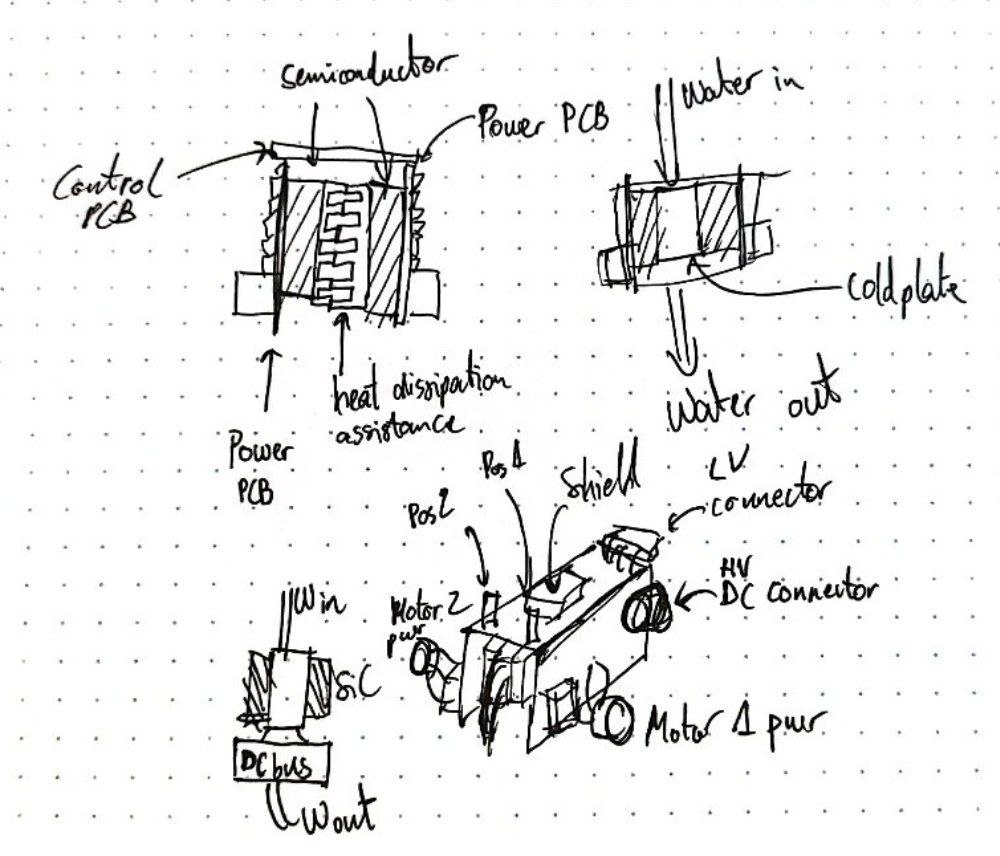
\includegraphics[width=\textwidth]{fig/boceto1}
	\end{minipage}\hfill
	\begin{minipage}{0.45\textwidth}
		\centering
		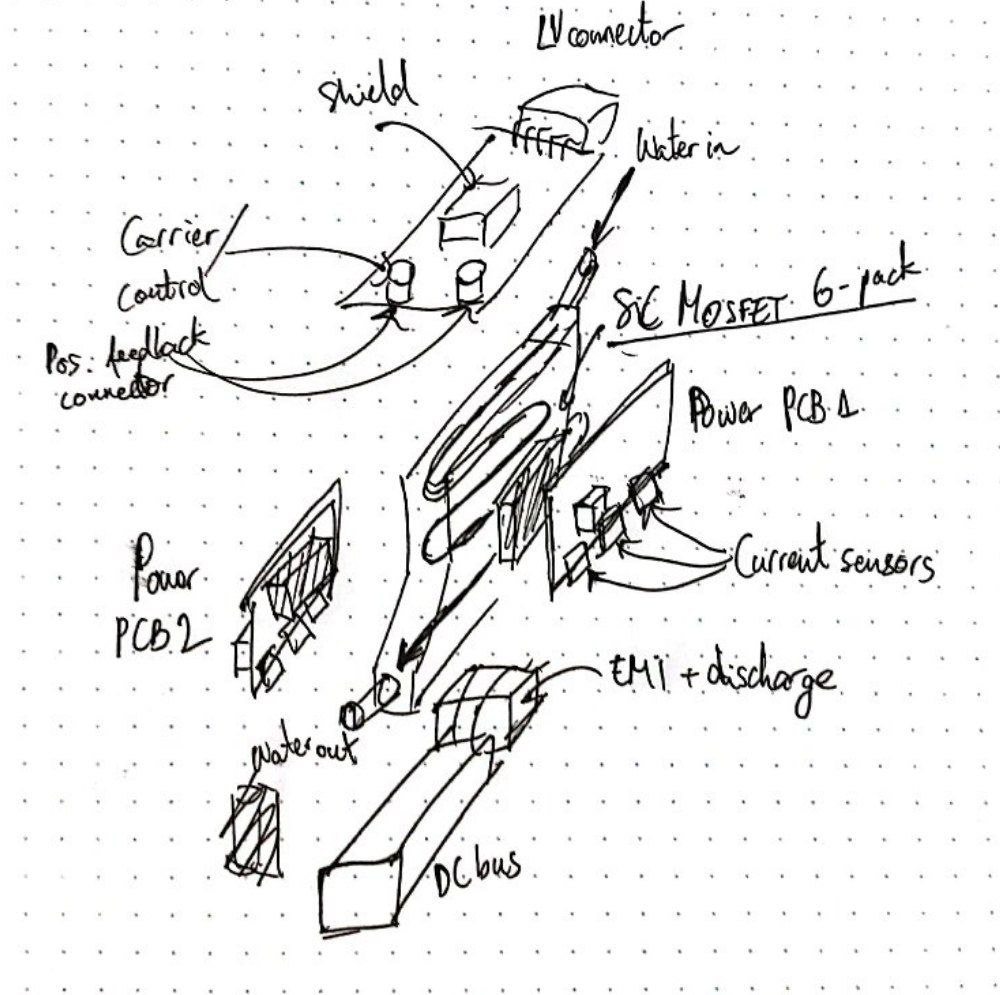
\includegraphics[width=\textwidth]{fig/boceto2}
	\end{minipage}
	\caption{Bocetos preliminares del empaquetado del inversor.}
\end{figure}

En estos dos primeros conceptos se explora el uso de una sola \textit{coldplate} para refrigerar ambos semiconductores. Adicionalmente se propone refrigerar el bus de condensadores, aunque posteriormente se encuentra que no es necesario. Se ha optado por una configuración que separa claramente los módulos de potencia de la placa de control, facilitando así el mantenimiento y la disipación de calor.

\begin{figure}[H]
	\centering
	\begin{minipage}{0.45\textwidth}
		\centering
		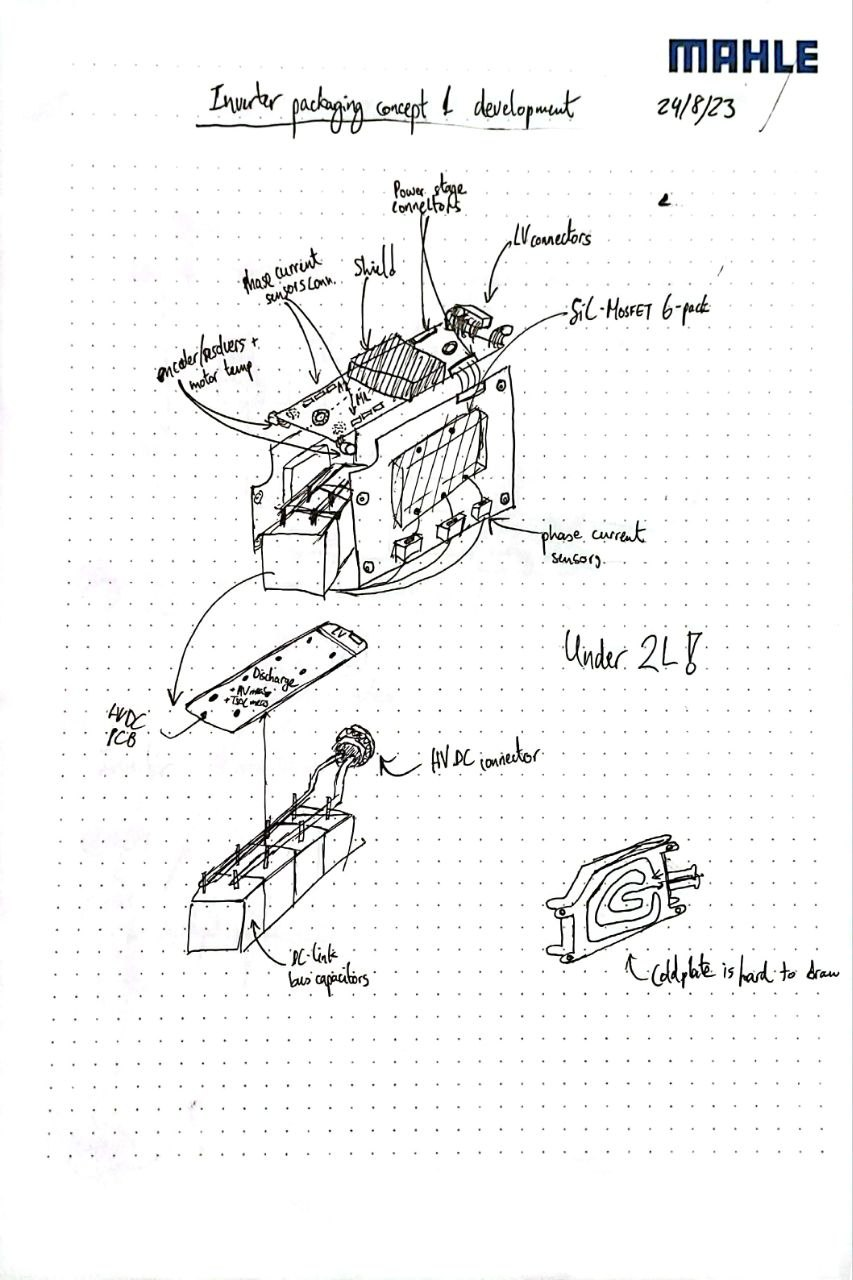
\includegraphics[width=\textwidth]{fig/boceto3}
	\end{minipage}\hfill
	\begin{minipage}{0.45\textwidth}
		\centering
		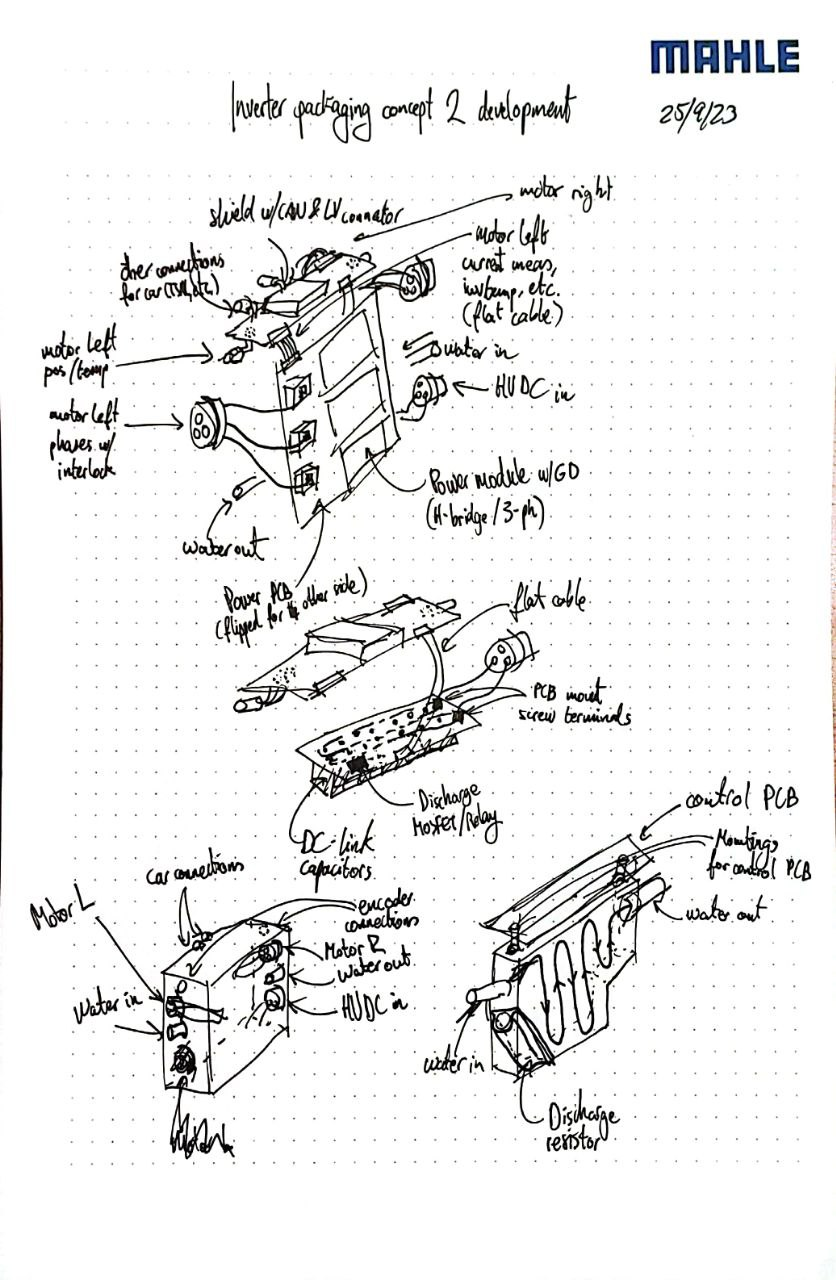
\includegraphics[width=\textwidth]{fig/boceto4}
	\end{minipage}
	\caption{Evolución de los bocetos del empaquetado del inversor.}
	\label{sketches}
\end{figure}

En los bocetos posteriores, se ha refinado la disposición de los componentes para mejorar la accesibilidad y la eficiencia de refrigeración. La disposición de los conectores y la distribución de los conductores también se ha ajustado para optimizar la densidad de potencia y la eficiencia del diseño. Estos cambios reflejan un enfoque hacia un empaquetado más eficiente y funcional del inversor. De todas maneras, todavía presentan muchas complicaciones en el ensamblaje y fabricación de algunos elementos como la \textit{coldplate}.

Estos bocetos iniciales proporcionan una idea visual de cómo se podría organizar el empaquetado del inversor. A medida que avanza el diseño, se realizarán ajustes a la vez que se encuentren limitaciones con los componentes específicos seleccionados y se hagan consideraciones eléctricas y térmicas que en este punto no se han tenido.

\subsection{Topología y concepto}
Con el fin de producir las tensiones trifásicas que calcula el control para los dos motores se implementa un ondulador trifásico fuente de voltaje doble (\textit{dual VSI}). Poniendo el foco en uno solo de los convertidores, existen varias topologías que permiten hacer un ondulador trifásico, pero la más utilizada es el VSI de 2 niveles, formado por tres ramas de medio puente. Otras topologías de más niveles logran sintetizar las tensiones con menos distorsión armónica, pero dado que el motor eléctrico es una carga inductiva, y que el control está basado en consignas de corriente, la distorsión armónica del convertidor tiene un impacto muy poco significativo en el rendimiento global. De esta manera, se justifica la implementación del VSI dual.

\begin{figure}[H]

    \centering
    \begin{circuitikz}
        % Upper MOSFETs
        \draw (0,0) node[nigfete,anchor=D,bodydiode] (M1) {};
        \draw (2,0) node[nigfete,anchor=D,bodydiode] (M2) {};
        \draw (4,0) node[nigfete,anchor=D,bodydiode] (M3) {};

        % Lower MOSFETs
        \draw (0,-2) node[nigfete,anchor=D,bodydiode] (M4) {};
        \draw (2,-2) node[nigfete,anchor=D,bodydiode] (M5) {};
        \draw (4,-2) node[nigfete,anchor=D,bodydiode] (M6) {};

        % Connections
        \draw (M1.S) -- (M4.D);
        \draw (M2.S) -- (M5.D);
        \draw (M3.S) -- (M6.D);
        \draw (M1.D) -- (M2.D) -- (M3.D);
        \draw (M4.S) -- (M5.S) -- (M6.S);

        % Battery
        \draw (M1.D)  |-  ++(-4,0) to[battery, l=$V_{\text{DC}}$] ++(0,-3.5)  |-  (M4.S);
        \draw (M1.D)  |-  ++(-1.5,0) to[capacitor] ++(0,-3.5)  |-  (M4.S);

        % Phase cables
        \draw (M3.S)  |-  ++(2,-0.5) node[right, font=\tiny] {C};
        \draw (M2.S)  |-  ++(4,-0.25) node[right, font=\tiny] {B};
        \draw (M1.S)  |-  ++(6,0) node[right, font=\tiny] {A};

    \end{circuitikz}
        \caption{VSI con MOSFETs.}

\end{figure}

Ya que el convertidor implementa código propio, se decide implementar dos VSI en el mismo convertidor, de modo que se opta por unificar algunos elementos de ambos como la refrigeración con el fin de optimizar el peso y el espacio. Esta decisión evita duplicados de medidas, componentes y código, sin embargo, conlleva otros retos, como por ejemplo, que el microcontrolador deberá ser capaz de ejecutar los dos lazos de control al mismo tiempo.

Para adquirir las variables necesarias para el control y la interfaz con el vehículo y sus periféricos, se requieren los submódulos que se presentan en el diagrama de bloques mostrado en la figura \ref{blocksHardware}.

\begin{figure}[H]
	\centering
	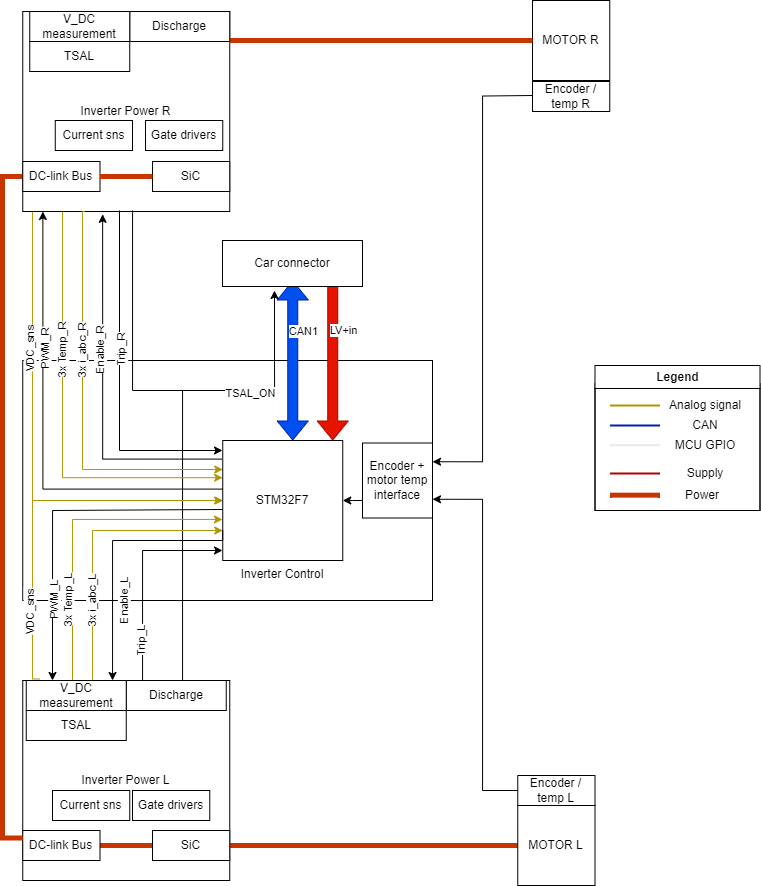
\includegraphics[width=0.7\linewidth]{fig/Inverter_HW}
	\caption{Diagrama de bloques del sistema completo.}
	\label{blocksHardware}
\end{figure}

El convertidor se divide en 3 PCBs, \textit{Inverter Power}, que se instala por duplicado (una por motor), e \textit{Inverter Control}. Como su nombre indica, \textit{Inverter Power} alojará todos los componentes de potencia, incluyendo los \textit{gate drivers}, los sensores de corriente, los semiconductores, el bus de condensadores y los conectores de potencia. Además, en esta placa se puede encontrar el sensado de la tensión de los buses, los circuitos de descarga, y la detección de alta tensión para la \textit{TSAL}. El sensado de tensión sería el único subcircuito repetido, pero esto solamente aporta redundancia y tolerancia al fallo.

Por su parte, \textit{Inverter Control} contiene el microcontrolador de la familia STM32F7 para consignar la conmutación a los \textit{gate drivers}, así como para realizar las lecturas de corriente, tensión y temperatura, las interfaces con los sensores de posición de los motores o los protocolos comunicación CAN y USB.

El montaje de estas placas se realiza de forma compacta y eficiente, de manera que cabe una \textit{coldplate} entre medias de las dos de potencia para refrigerar los semiconductores de ambos inversores. Se encajan de manera que la placa de control se puede conectar a las placas de potencia mediante conectores placa a placa. Las conexiones de potencia facilitan la integración con el cableado del monoplaza debido a su posicionamiento.


\subsection{Semiconductores}

\subsubsection{Tecnología de semiconductores}

La decisión de emplear MOSFETs de carburo de silicio (SiC) como interruptores se fundamenta en consideraciones específicas de la aplicación y en los requisitos de la competición. En un entorno donde la reducción de peso y volumen es crucial, el SiC emerge como una opción destacada frente a alternativas como el IGBT de silicio, el FET de GaN o el MOSFET de silicio. Aunque el precio no es una limitación primordial en este caso, el proyecto ha atraído el interés de empresas que han ofrecido muestras de semiconductores de forma gratuita para el desarrollo del convertidor.

Las ventajas inherentes del SiC, como su rendimiento superior o su resistencia a temperaturas más altas, permiten un diseño más compacto y robusto del inversor de tracción. Estas características son esenciales para cumplir con los requisitos de un monoplaza de competición, donde lograr altas densidades de potencia es muy beneficioso para la integración del resto de componentes del vehículo y aligeramiento del mismo.

\subsubsection{Módulos de potencia}

En el diseño del inversor de tracción, se optó por módulos \textit{half-bridge} debido a su idoneidad para el rango de potencias y tensiones del convertidor. Dos modelos de semiconductores se consideraron para su integración: el DFS05HF12EYR1 de Leapers Semiconductor y el CAB016M12FM3 de Wolfspeed.

Ambos modelos cumplen estrictamente con los requisitos de la aplicación, con un voltaje de ruptura (\(V_{\text{DS,breakdown}}\)) de 1200 V y una corriente máxima (\(I_{\text{DS,máx}}\)) que excede los 80 A,RMS. La elección de dos modelos distintos se basa en la intención de realizar pruebas comparativas para verificar las diferencias entre ambos.

El DFS05HF12EYR1 ofrece especificaciones muy buenas en su datasheet, aunque Leapers Semiconductors no lleva muchos años en la industria y no han logrado crear la confianza que otras empresas han conseguido con su experiencia. Por otro lado, el CAB016M12FM3, de la reconocida marca Wolfspeed (antiguamente CREE), aporta la confiabilidad asociada a una empresa con amplia experiencia en el campo.

Según sus respectivos datasheets, ambos modelos permiten alcanzar sin mucho esfuerzo una frecuencia de conmutación de 40 kHz, lo que contribuye significativamente a la reducción del tamaño del bus de continua y optimiza el empaquetado del inversor. La placa de potencia se diseñará para permitir la prueba de ambos modelos, ya que comparten \textit{footprint}, facilitando la adaptabilidad y la evaluación comparativa.

\begin{table}[H]
	\centering
	\begin{tabular}{|l|l|l|}
		\hline
		\textbf{Parámetro} & \textbf{DFS05HF12EYR1} & \textbf{CAB016M12FM3} \\ \hline
		\(V_{\text{DS,breakdown}}\) [V] & 1200 & 1200 \\ \hline
		\(R_{\text{on}}\) [\(\text{m} \Omega\)] & 5.5 - 13 & 16.0 - 28.8 \\ \hline
		\(V_{\text{f,D}}\) [V] & 3.3 - 4 & 4.9 - 5.5 \\ \hline
		\(T_{\text{rr}}\) [ns] & 41.5 - 45 & 20.0 \\ \hline
		\(Q_{\text{rr}}\) [\unit{\micro\coulomb}] & 2.19 - 3.94 & 1.30 \\ \hline
		\(R_{\text{th,jc}}\) [K/W] & 0.12 - 0.15 & 0.543 \\ \hline
		\(Q_{\text{G}}\) [\(n\text{C}\)] & 520 & 236 \\ \hline
		\(C_{\text{in}}\) [nF] & 14.5 & 6.6 \\ \hline
		\(R_{\text{G,int}}\) [\(\Omega\)] & 1.9 & 2.4 \\ \hline
		\(V_{\text{GS,th}}\) [V] & 2.8 - 4.8 & 1.8 - 3.6 \\ \hline
		\(I_{\text{DS,máx}}\) [A] & 150 & 89 \\ \hline
		& 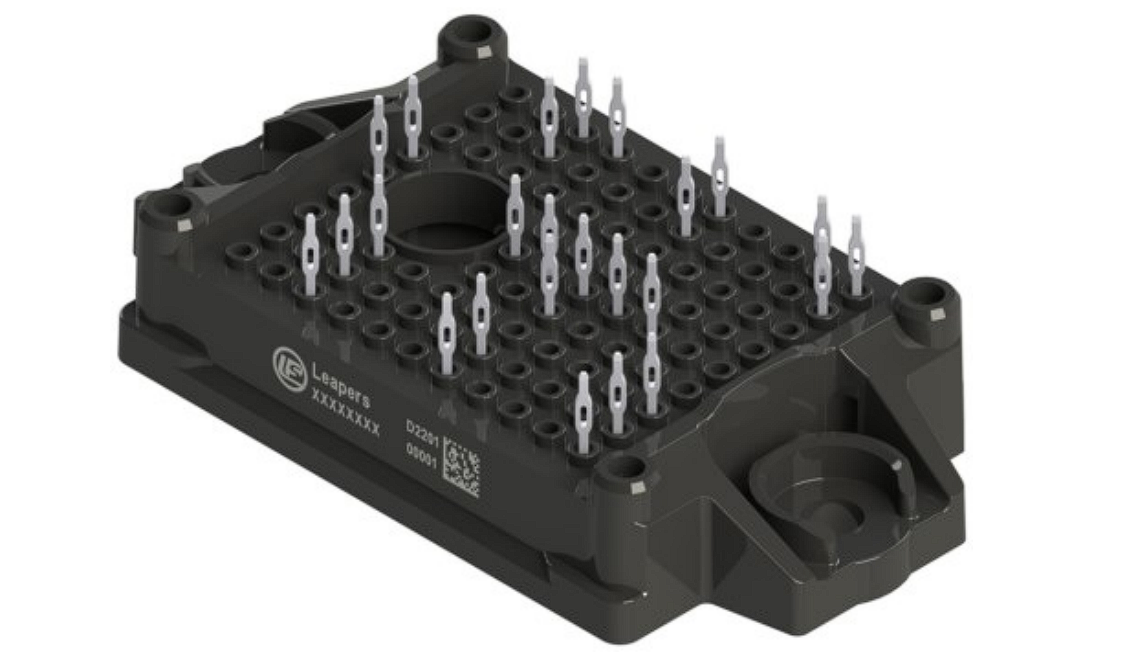
\includegraphics[width=0.2\textwidth]{fig/DFS05.png} & \includegraphics[width=0.2\textwidth]{fig/CAB016.png} \\
		\hline
	\end{tabular}
	\caption{Comparación de parámetros entre DFS05HF12EYR1 y CAB016M12FM3.}
\end{table}

\subsubsection{Análisis de pérdidas}

Los dispositivos semiconductores experimentan pérdidas de energía que influyen significativamente en su eficiencia y desempeño, y se transforman en calor, limitando así la potencia de salida. Estas pérdidas pueden clasificarse en dos categorías fundamentales: las pérdidas de conducción y las pérdidas de conmutación. Las \textbf{pérdidas de conducción} surgen cuando el dispositivo se encuentra en estado activo, conduciendo corriente a través de él. Esto genera una caída de voltaje y una disipación de potencia asociada a la resistencia interna del dispositivo. Por otro lado, las \textbf{pérdidas de conmutación} se manifiestan durante los ciclos de activación y desactivación del dispositivo, cuando la energía almacenada en la capacitancia del mismo se disipa durante la transición entre los estados de conducción y corte.

En el análisis de la eficiencia de los semiconductores, es imperativo considerar las pérdidas totales, las cuales se definen como la suma de las pérdidas de conducción y las de conmutación:

\begin{equation}
	P_{\text{tot}} = P_{\text{cond}} + P_{\text{conm}}
\end{equation}

A continuación, se examinarán detalladamente las pérdidas de conducción, seguidas por un análisis exhaustivo de las pérdidas de conmutación en los módulos seleccionados.


\textbf{Pérdidas de conducción}

Las pérdidas de conducción tienen su origen en la resistencia entre drenador y fuente cuando el MOSFET está en estado de conducción, o en la caída de tensión del diodo cuando es el diodo quien está conduciendo. Según la ley de Ohm 

\begin{equation}
P_{\text{cond,MOSFET}}= I_{\text{DS}}^2\cdot R_{\text{DS, on}}\text{,}
\end{equation}
y la definición de potencia
\begin{equation}
P_{\text{cond},D} = I_{\text{SD}}\cdot V_\text{f}\text{.}
\end{equation}

Sin embargo, estas expresiones se corresponden con las pérdidas instantáneas y no son útiles a la hora de dimensionar el convertidor. Para ello son necesarias las pérdidas promediadas, pero tienen una expresión analítica muy compleja, ya que dependen de la estrategia de modulación, el índice de modulación instantáneo, el factor de potencia instantáneo, etc. Para el inversor se utiliza SVPWM, pero el cálculo de pérdidas tiene demasiados parámetros instantáneos. Muchas referencias asemejan las pérdidas en SVPWM a las de una modulación PWM sinusoidal (SPWM), con lo que las pérdidas se simplifican \cite{Gross2018}.

\begin{equation}
P_{\text{cond,MOSFET}} \approx I_{\text{RMS}} V_{\text{Q0}} \left(\frac{1}{\pi\sqrt{2}} + \frac{m\cdot cos(\phi)}{2\sqrt{8}}\right) + I_{\text{RMS}}^2 R_\text{Q} \left(\frac{1}{4} + \frac{2\cdot m}{3\pi\cdot cos(\phi)}\right)
\end{equation}

\begin{equation}
P_{\text{cond,D}} \approx I_{\text{RMS}} V_{\text{D0}} \left(\frac{1}{\pi\sqrt{2}} - \frac{m\cdot cos(\phi)}{2\sqrt{8}}\right) + I_{\text{RMS}}^2 R_\text{D} \left(\frac{1}{4} - \frac{2\cdot m}{3\pi\cdot cos(\phi)}\right)
\end{equation}

Como se puede apreciar, aunque son más compactas que otras en la bibliografía, estas expresiones son difíciles de abordar, puesto que casi todos los parámetros son instantáneos. Por ello, se ha usado PLECS para estimar las pérdidas de conducción debido a que facilita la simulación detallada de los semiconductores y permite obtener las pérdidas de forma diseccionada por cada dispositivo y tipo de pérdida. PLECS utiliza modelos detallados de los dispositivos, considerando sus características de conmutación y conducción reales.

Con los parámetros de estos modelos, PLECS calcula las pérdidas de conmutación y conducción de manera precisa. Sin embargo, como no tiene en cuenta el circuito completo de los \textit{gate drivers}, no se pueden tomar directamente las pérdidas de conmutación. Se usa un modelo de MOSFET y diodo de Wolfspeed proporcionado directamente por el fabricante. Este modelo cuenta con una parametrización de las pérdidas y los efectos térmicos mucho más detallada que la que se puede obtener a partir de la hoja de datos. El fabricante utiliza tablas de búsqueda en función de la tensión, corriente y temperatura, e incorpora una relación matemática con las resistencias de puerta. Lamentablemente, Leapers no ofrece esta parametrización con sus semiconductores, por lo que el análisis en PLECS se realiza únicamente con el modelo de Wolfspeed, siendo este el más restrictivo en cuanto a las pérdidas de conducción.

Para sacarle el máximo partido, se ha obtenido un perfil de pérdidas a máxima potencia para el inversor en diferentes zonas de control del PMSM, que se puede observar a continuación.

\begin{figure}[H]
	\centering
	\includegraphics[width=0.9\linewidth]{fig/PLECS-invLosses}
	\caption{Descomposición de las pérdidas de los semiconductores de una simulación en PLECS.}
	\label{losses-sim}
\end{figure}

Se puede ver como las pérdidas de conducción son más significativas que las de conmutación, en particular, las de los MOSFETs. Las zonas de par constante (de 1,05 s a 1,4 s por ejemplo), muestran unas pérdidas casi constantes con la corriente, pero crecen debido a la temperatura. Al entrar en la zona de límite de tensión (de 1,7 s a 1,8 s), se observa un pico que se corresponde con la zona de potencia constante, que en esta simulación es la potencia máxima. Para obtener un valor constante de pérdidas con el que diseñar la refrigeración, se parte de este valor de pico (450 W aproximadamente) y se trata de la misma manera que la relación de potencia media respecto a la potencia pico calculada en la sección de requisitos.

\[
\frac{P_{\text{RMS}}}{P_{\text{pico}}} = \frac{35\text{ kW}}{80\text{ kW}} = 0.4375 \approx 0.5
\]

Con este razonamiento, se da un valor de pérdidas de conducción máximas de un inversor de $450 \text{W} \cdot 0.5 = 225 \text{ W}$. Como hay dos inversores anclados a la misma \textit{coldplate}, las pérdidas de conducción que debe disipar es de $225 \text{ W} \cdot 2 = 450 \text{ W}$. Es importante recordar que estas pérdidas son para el semiconductor de Wolfspeed. Dado que las pérdidas de conducción son proporcionales a $R_{\text{DS, on}}$, se pueden aproximar las pérdidas de conducción del semiconductor de Leapers.
\[
P_{\text{cond,Wolfspeed}} = 450 \text{ W}
\]

\[
P_{\text{cond,Leapers}} \approx P_{\text{cond,Wolfspeed}} \cdot \frac{R_{\text{DS, on, Leapers}}}{R_{\text{DS, on, Wolfspeed}}} = 450 \text{ W} \cdot \frac{5.5 \text{ m}\Omega}{16 \text{ m}\Omega} \approx 155 \text{ W}
\]


\textbf{Pérdidas de conmutación}

El cálculo de las pérdidas de conmutación es más fácil de determinar de forma analítica, aunque depende del circuito de \textit{gate driver} y de sus parásitos. Si no se tienen en cuenta estos dos factores, se pueden calcular utilizando los valores de \(E_{\text{on}}\) y \(E_{\text{off}}\), que representan la energía necesaria para encender o apagar el dispositivo respectivamente. Cuando las hojas de datos de los semiconductores proporcionan los valores \(E_{\text{on}}\) y \(E_{\text{off}}\), las pérdidas de conmutación pueden calcularse de forma directa. Estas pérdidas están influenciadas por la tensión de conmutación, la corriente de conmutación, la temperatura de la unión y la resistencia de puerta. La fórmula comúnmente utilizada para calcular las pérdidas es

\begin{equation}
E_{\text{conm}}(t) = (E_{\text{on}} + E_{\text{off}}) \left( \frac{I_{\text{Q,env}}(t)}{I_{\text{test}}} \right)^{K_i} \left( \frac{V_{\text{DC}}}{V_{\text{test}}} \right)^{K_v} \text{,}
\end{equation}

donde \(I_{\text{Q,env}}(t)\) es la corriente de conmutación en cada instante de tiempo, \(I_{\text{test}}\) y \(V_{\text{test}}\) son los valores de prueba, y \(K_i\) y \(K_v\) son coeficientes de ajuste que normalmente son igual a 1. La justificación se puede encontrar en los gráficos proporcionados en las hojas de datos de ambos semiconductores, donde la relación de las energías de encendido y apagado con la corriente es aproximadamente lineal.

\begin{figure}[H]
	\centering
	\begin{subfigure}[b]{0.4\linewidth}
		\centering
		\includegraphics[width=\linewidth]{fig/eoneoffleapers}
		\caption{Leapers}
	\end{subfigure}
	\hfill
	\begin{subfigure}[b]{0.55\linewidth}
		\centering
		\includegraphics[width=\linewidth]{fig/eoneoffwolfspeed}
		\caption{Wolfspeed}
	\end{subfigure}
	\caption{Energías de encendido y apagado en función de la corriente para Leapers \cite{DFS05HF12EYR1} y Wolfspeed \cite{CAB016M12FM3}.}
\end{figure}

Si la corriente es continua,

\begin{equation}
P_{\text{conm}} \approx (E_{\text{on}} + E_{\text{off}}) f_{\text{conm}} \frac{I_{\text{out}}}{I_{\text{test}}} \frac{V_{\text{DC}}}{V_{\text{test}}} \text{.}
\end{equation}

Y si la corriente es una sinusoide semi-rectificada con un valor de pico de \(\sqrt{2} I_{\text{RMS}}\) (como en el caso del SVPWM), 

\begin{equation}
P_{\text{conm}} \approx (E_{\text{on}} + E_{\text{off}}) f_{\text{conm}} \frac{\sqrt{2} I_{\text{RMS}}}{\pi I_{\text{test}}} \frac{V_{\text{DC}}}{V_{\text{test}}}\text{.}
\end{equation}

Para obtener los valores de $E_{\text{on}}$ y $E_{\text{off}}$ se pueden usar los gráficos que aparecen en las hojas de datos, ya que principalmente dependen de la resistencia de puerta que se escoja.

\begin{figure}[H]
	\centering
	\begin{subfigure}[b]{0.4\linewidth}
		\centering
		\includegraphics[width=\linewidth]{fig/eoneoffleapers_RG}
		\caption{Leapers}
	\end{subfigure}
	\hfill
	\begin{subfigure}[b]{0.55\linewidth}
		\centering
		\includegraphics[width=\linewidth]{fig/eoneoffwolfspeed_RG}
		\caption{Wolfspeed}
	\end{subfigure}
	\caption{Energías de encendido y apagado en función de la resistencia de puerta externa para Leapers \cite{DFS05HF12EYR1} y Wolfspeed \cite{CAB016M12FM3}.}
\end{figure}

Se escogerán los valores más grandes de resistencia de puerta para hacer este cálculo, pues un valor más grande produce menos sobrepico de tensión en la conmutación, pero aumenta las pérdidas. Sustituyendo por los valores del convertidor en diseño,

\begin{itemize}
	\item Generales: \(f_{\text{conm}} = 40 \text{ kHz}\), \(I_{\text{RMS}} = 80 \text{ A}\), \(V_{\text{DC}} = 600 \text{ V}\)
	\item Leapers: \(E_{\text{on}} = 5.8 \text{ mJ}\), \(E_{\text{off}} = 3.7 \text{ mJ}\), \(V_{\text{test}} = 600 \text{ V}\), \(I_{\text{test}} = 150 \text{ A}\)
	\item Wolfspeed: \(E_{\text{on}} = 1.8 \text{ mJ}\), \(E_{\text{off}} = 0.9 \text{ mJ}\), \(V_{\text{test}} = 600 \text{ V}\), \(I_{\text{test}} = 80 \text{ A}\)
\end{itemize}

Sustituyendo para los dispositivos Leapers,

\[
P_{\text{conm, Leapers}} \approx (5.8 \text{ mJ} + 3.7 \text{ mJ}) \cdot 40 \text{ kHz} \cdot \frac{80 \text{ A}}{150 \text{ A}} \cdot \frac{600 \text{ V}}{600 \text{ V}} \approx 91.23 \text{ W,}
\]

y para los dispositivos Wolfspeed,

\[
P_{\text{conm, Wolfspeed}} \approx (1.8 \text{ mJ} + 0.9 \text{ mJ}) \cdot 40 \text{ kHz} \cdot \frac{80  \text{ A}}{80 \text{ A}} \cdot \frac{600 \text{ V}}{600 \text{ V}} \approx 48.61 \text{ W.}
\]

Dado que estas pérdidas son para un solo MOSFET, se deben multiplicar por 12 para obtener las pérdidas de conmutación totales, dado que hay 6 dispositivos de potencia en la topología VSI y hay dos VSIs en el convertidor.

\[
P_{\text{conm, Leapers, tot}} = 12\cdot P_{\text{conm, Leapers}} \approx 1095 \text{ W}
\]

\[
P_{\text{conm, Wolfspeed, tot}} = 12\cdot P_{\text{conm, Wolfspeed}} \approx 583 \text{ W}
\]


\textbf{Resumen de pérdidas}

El siguiente gráfico presenta una comparación detallada de las pérdidas de conducción y conmutación para los semiconductores de Leapers y Wolfspeed.

\begin{figure}[H]
	\centering
	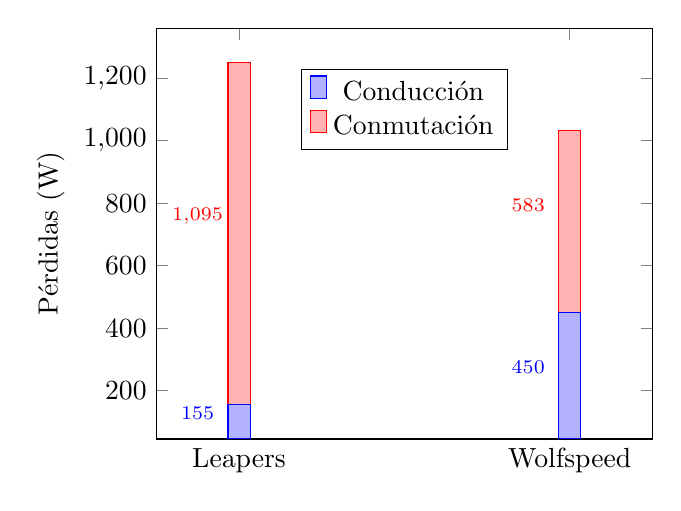
\begin{tikzpicture}
		\begin{axis}[
			ybar stacked,
			width=0.65\textwidth,
			yticklabel style={/pgf/number format/.cd,fixed,fixed zerofill,precision=0,/tikz/.cd},
			ylabel={Pérdidas (W)},
			symbolic x coords={Leapers, Wolfspeed},
			xtick=data,
			bar width=8pt, % Ancho de las barras
			enlarge x limits=0.25, % Espacio adicional a ambos lados de las barras
			nodes near coords,
			nodes near coords align={vertical},
			every node near coord/.append style={font=\scriptsize, xshift=-15pt, yshift=0pt},
			legend style={
				at={(0.5, 0.9)},
				anchor=north,
			},
			]
			\addplot coordinates {(Leapers, 155) (Wolfspeed, 450)};
			\addplot coordinates {(Leapers, 1095) (Wolfspeed, 583)};
			\legend{Conducción, Conmutación}
		\end{axis}
	\end{tikzpicture}
	\caption{Comparación de pérdidas de conducción y conmutación.}
	\label{fig:loss_comparison}
\end{figure}

\begin{table}[H]
	\centering
	\begin{tabular}{|c|p{3.5cm}|p{3.5cm}|p{3.5cm}|}
		\hline
		\textbf{Fabricante} & \textbf{Pérdidas de conducción (W)} & \textbf{Pérdidas de conmutación (W)} & \textbf{Pérdidas totales (W)} \\
		\hline
		Leapers & 155 & 1095 & 1250 \\
		\hline
		Wolfspeed & 450 & 583 & 1033 \\
		\hline
	\end{tabular}
	\caption{Comparación de pérdidas entre semiconductores.}
\end{table}

Se observa que en el caso de Leapers, las pérdidas de conducción exhiben una significativa disminución en comparación con las de Wolfspeed, mientras que las pérdidas de conmutación muestran un incremento dramático para Leapers en relación con Wolfspeed. Este fenómeno sugiere que, en líneas generales, los dispositivos desarrollados por Leapers podrían ofrecer un camino de corriente más favorable en el semiconductor, y los dispositivos de Wolfspeed son capaces de conmutar más rápido debido a que su carga $Q_{\text{G}}$ es mucho menor, reduciendo así $E_{\text{on}}$ y $E_{\text{off}}$. Para el uso de los semiconductores de Leapers se recomienda bajar la frecuencia de conmutación, prestando atención a las afectaciones que pudiera tener en el bus de continua y en el control. El desarrollo práctico del trabajo se enfocará en los semiconductores de Wolfspeed por parecer una opción más equilibrada para la aplicación.

La suma total de las pérdidas de ambos inversores, independientemente del semiconductor, es como máximo de 1300 W, valor con el cual se puede diseñar el sistema de refrigeración.

\subsection{Sistema de refrigeración}

A continuación se presenta una comparación entre las opciones comunes para refrigerar el inversor:

\begin{table}[H]
	\centering
	\begin{tabular}{|p{2.5cm}|p{5cm}|p{5cm}|}
		\hline
		\textbf{Opción de refrigeración} & \textbf{Ventajas} & \textbf{Desventajas} \\ \hline
		Convección natural & Económica, sin partes móviles & Limitada disipación de calor, depende del ambiente \\ \hline
		Disipador de calor & Económico, fácil de instalar, no requiere energía adicional & Limitado en aplicaciones de alta potencia, depende del ambiente \\ \hline
		Ventilador & Buena disipación de calor, control de temperatura & Limitado en aplicaciones de alta potencia, ruido \\ \hline
		\textit{Coldplate} de agua & Excelente capacidad de disipación, buen control de temperatura & Coste, mantenimiento, posible riesgo de fugas, instalación complicada \\ \hline
		\textit{Coldplate} de aceite & Buena capacidad de disipación, no corrosivo, alto rango de temperaturas &  coste, mantenimiento, posible riesgo de fugas, instalación complicada \\ \hline
	\end{tabular}
	\caption{Comparación de opciones de refrigeración.}
\end{table}



Para el sistema de refrigeración de los semiconductores se ha optado por un sistema de refrigeración líquida consistente en una \textit{coldplate}, una bomba y un radiador. Esta elección se basa en varios factores clave que se detallan a continuación:

\begin{itemize}
	\item \textbf{Mantenimiento de la temperatura:} A diferencia de una refrigeración por aire, una \textit{coldplate} permite mantener una interfaz de temperatura fija para los semiconductores. Esto es crucial para garantizar un funcionamiento estable y confiable de los componentes, especialmente en aplicaciones de alta potencia como la que se está diseñando.
	
	\item \textbf{Experiencia previa:} El equipo tiene experiencia previa en sistemas de refrigeración líquida, lo que facilita la implementación y mantenimiento de este tipo de sistemas.
	
	\item \textbf{Flexibilidad del \textit{packaging}:} La refrigeración líquida, especialmente con agua, permite un diseño más compacto en comparación con otras opciones. Un disipador haría mucho más voluminoso el convertidor, mientras que la refrigeración líquida permite una distribución más libre de los componentes por el monoplaza. Por ejemplo, se puede situar el radiador en una zona donde tenga mucho contacto con el aire exterior, y conectarlo mediante mangueras a la bomba y a la \textit{coldplate}.
	
	
\end{itemize}

Aunque el carburo de silicio tiene una temperatura máxima de la unión notablemente alta que el silicio, se ha establecido un objetivo de mantener la interfaz térmica del semiconductor a 80 $\si{\degreeCelsius}$ como máximo. Este enfoque busca garantizar una operación óptima y una vida útil prolongada de los semiconductores, además de mitigar los posibles efectos negativos derivados del calor.

Se ha elegido agua como el fluido de refrigeración por varias razones:

\begin{itemize}
	\item \textbf{Norma T7.2.2:} Según la norma \textbf{\textit{T7.2.2}} \cite{FSG}, los sistemas de refrigeración solo pueden utilizar agua, aire u aceite como refrigerante. Con lo cual, no es posible utilizar líquidos refrigerantes específicos.
	
	\item \textbf{Propiedades térmicas:} El agua tiene una alta capacidad calorífica y conductividad térmica, lo que la hace eficaz para disipar el calor generado por los semiconductores. El aceite tiene peor conductividad térmica, y su amplio rango de temperaturas no es útil para la aplicación.
	
	\item \textbf{Seguridad:} El agua es un fluido seguro y no inflamable, lo que reduce los riesgos de seguridad en caso de fugas o accidentes. Además, es un fluido fácilmente disponible y de bajo costo en comparación con otros refrigerantes. Si se usa agua destilada, el riesgo de corrosión es más bajo, y los sistemas electrónicos no serán tan susceptibles a posibles fugas.
	
\end{itemize}

En el presente trabajo no se desarrolla más acerca el sistema de refrigeración puesto que la complejidad de diseñarlo excede el alcance del proyecto. Sin embargo, se reconoce su importancia, ya que al no disponer de este no se pueden realizar pruebas de potencia constante.

\subsection{\textit{Gate drivers}}

Los gate drivers son componentes críticos en un convertidor de potencia, puesto que son los encargados de conectar las señales débiles de un microcontrolador con los semiconductores. Además, suelen llevar funcionalidades adicionales como la detección de cortocircuitos en el semiconductor, la lectura de señales analógicas de forma aislada, o mecanismos de protección avanzados.

\subsubsection{Funcionamiento genérico}

Los \textit{gate drivers} desempeñan un papel esencial en la conmutación eficiente de los MOSFETs, proporcionando los niveles de tensión y corriente adecuados para activar y desactivar rápidamente los transistores. En esencia, es una etapa transistorizada que "amplifica" la fuerza de la señal del microcontrolador, y a menudo lo hace de forma aislada.

\subsubsection{Criterios de selección}

Al seleccionar un \textit{gate driver}, varios factores deben tenerse en cuenta para garantizar un rendimiento óptimo del sistema:

\begin{itemize}
	\item \textbf{Topología}: A pesar de que hay soluciones que incluyen 6 \textit{drivers} en un solo encapsulado, las más comunes son los circuitos integrados diseñados para controlar un solo dispositivo o dos en configuración de medio puente. Sin embargo, encontrar esta última opción para el rango de tensiones de 600 V con características óptimas es difícil. Por lo tanto, la topología más adecuada suele ser la de un solo \textit{driver} por encapsulado.
	\item \textbf{Tensión de aislamiento}: Dado que las señales de puerta vienen del sistema de baja tensión, deben aislarse antes de llegar al \textit{gate}, con lo que será necesario buscar un componente aislado a una tensión adecuada de al menos tres veces superior a la tensión máxima del inversor, 600 V. 
	\item \textbf{Corriente de salida}: Es crucial elegir un \textit{gate driver} que pueda suministrar la corriente necesaria para cargar y descargar rápidamente las capacidades de compuerta de los MOSFETs. La corriente necesaria depende de la resistencia de puerta, pero se puede determinar una primera cota de $\frac{V_{\text{GS,typ}}}{R_{\text{G,int}}} = \frac{20 \text{ V}}{2.4 \text{ }\Omega} = 8.3 \text{ A}$
	\item \textbf{Protecciones integradas}: Funciones como la lectura de señales analógicas, la posibilidad de paralelizar salidas o la inclusión de protecciones son muy beneficiosas para la integración del convertidor.
\end{itemize}

\subsubsection{Comparativa de alternativas}

A continuación se presenta una comparativa entre varios modelos de \textit{gate drivers}, considerando sus características principales:

\begin{table}[H]
	\centering
	\begin{tabular}{|l|p{3.5cm}|p{3.5cm}|p{3.5cm}|}
		\hline
		\textbf{Características} & \textbf{ADUM4146} & \textbf{UCC21710} & \textbf{GD3160} \\
		\hline
		Voltaje de Operación & -15 V hasta 30 V & –17,5 V hasta 36 V & -12 V hasta 25V \\
		\hline
		Corriente de Salida & 4,61 A & 10 A & 15 A \\
		\hline
		Protecciones & Desaturación, UVLO & Sobrecorriente, Desaturación, \textit{Miller Clamp} & Desaturación, Sobrecorriente, Apagado suave \\
		\hline
		Tiempo de Retardo & 75 ns & 90 ns & - \\
		\hline
		Aislamiento & 5 kV & 5,7 kV & 8 kV \\
		\hline
		Extras & - & Sensor analógico aislado & Sensor analógico aislado \\
		\hline
		CMTI & 100 V/ns & 150 V/ns & 100 V/ns \\
		\hline
	\end{tabular}
	\caption{Comparación de \textit{gate drivers}.}
\end{table}

Considerando los criterios de selección, se observa que el UCC21710 se presenta como una opción intermedia adecuada. En primer lugar, la corriente de salida que ofrece es de hasta 10 A, lo que lo hace adecuado para cargar y descargar rápidamente las capacidades de compuerta de los MOSFETs, cumpliendo así con uno de los requisitos fundamentales. Además, integra protecciones contra sobrecorriente y desaturación, así como la funcionalidad de \textit{Miller Clamp}. Además, la inclusión de un sensor analógico aislado proporciona la capacidad de monitorear la temperatura de los semiconductores con sus sensores integrados sin ningún componente adicional.

Aunque las protecciones de sobrecorriente y desaturación son elementos fundamentales para garantizar la seguridad y el correcto funcionamiento de un inversor, en este caso se ha optado por no implementarlas debido a las complicaciones que pueden surgir en el diseño del \textit{layout}. Estas protecciones requieren la inclusión de componentes adicionales con \textit{footprints} grandes y un enrutamiento más complejo de las señales, lo cual puede resultar en problemas de interferencia y aumento de la complejidad del circuito.

Es importante destacar que este inversor se encuentra en una fase inicial de prototipado y desarrollo, donde se prioriza la funcionalidad básica y la viabilidad del diseño. En futuras revisiones y etapas de desarrollo, se considerará la inclusión de estas protecciones, ya que son cruciales para proteger tanto el inversor como los dispositivos conectados. La decisión actual de omitir estas protecciones se basa en la necesidad de simplificar el diseño y garantizar una implementación más eficiente y manejable en esta fase del proyecto.

\begin{figure}[H]
	\centering
	\includegraphics[width=0.7\linewidth]{fig/UCC21710-block}
	\caption{Diagrama de bloques funcional del \textit{gate driver} seleccionado \cite{UCC21710}.}
\end{figure}


\subsubsection{Cálculos del \textit{gate driver} seleccionado}


\begin{itemize}
	
	\item \textbf{Tensión \textit{gate-source}}: Uno de los valores más importantes a determinar es el nivel de tensión de puerta para encender y apagar el MOSFET. En una aplicación \textit{hard-switched} como la del convertidor en diseño, es beneficioso usar una tensión de encendido tan alta como sea posible.
	
	Dada la naturaleza rápida del carburo de silicio, se prevé una dV/dt considerable, la cual puede causar varios problemas. Uno de ellos sería la activación accidental de un MOSFET, la cual causaría la condición de \textit{shoot-through}. Una estrategia para mitigar parcialmente este problema es el uso de un \textit{gate driver} con \textit{Miller Clamp}. Además, se suele apagar el dispositivo utilizando una tensión negativa, que amortigua posibles interferencias en la puerta del dispositivo afectado. El valor de tensión negativo al cual se encuentre la puerta aumenta la tensión que debe inducirse en ese nodo para llegar a la tensión umbral $V_{\text{G,treshold}}$ del MOSFET. Dado que el valor óptimo no es trivial, conviene implementar alguna manera de modificarlo, por ejemplo, mediante el uso de un regulador lineal.
	
	Los dispositivos seleccionados tienen un rango de tensiones $V_{\text{GS}}$ un tanto distintos, siendo el de Leapers de +21 V a -2 V, y el de Wolfspeed de +15 V a -4 V.
	
	\item \textbf{Potencia de alimentación del \textit{gate driver}:} Se estima en función de la frecuencia de conmutación y la carga de la compuerta de los MOSFETs, además de la tensión $V_{\text{GS}}$.
	
	\begin{equation}
	I_{\text{supply, min}} = f_{\text{conm}} \cdot Q_{\text{G}}
	\end{equation}
	
	Donde\\
	- \( I_{\text{supply, min}} \) es al corriente mínima que debe poder suministrar la fuente de alimentación del \textit{gate driver},\\
	- \( f_{\text{conm}} \) es la frecuencia de conmutación, y\\
	- \( Q_{\text{G}} \) es la carga en la puerta.\\
	
	Utilizando el valor más alto de $Q_{\text{G}}$ entre los dos semiconductores,
	\[
	I_{\text{supply, min}} = f_{\text{conm}}\cdot Q_{\text{G}} = 40 \text{ kHz} \cdot 520 \text{ nC} = 20.8 \text{ mA}
	\]
	
	se puede calcular la potencia necesaria de la fuente.
	
	\begin{equation}
		P_{\text{supply, min}} = \Delta V_{\text{GS}}\cdot I_{\text{supply, min}} 	
	\end{equation}
	
	Donde:\\
	- \( P_{\text{supply, min}} \) es la potencia mínima que debe poder suministrar la fuente de alimentación del \textit{gate driver} y\\
	- \( \Delta V_{\text{GS}} \) es la diferencia entre la tensión de puerta de encendido y apagado.\\
	
	\[
	P_{\text{supply, min}} = \Delta V_{\text{GS}}\cdot I_{\text{supply, min}} = 20 \text{ V} \cdot20.8 \text{ mA} = 0.416 \text{ W}
	\]
	
	Con esta estimación de potencia mínima requerida, es esencial seleccionar una fuente adecuada para los \textit{gate drivers}. En este contexto, se considera la serie MGJ2 de Murata, que ofrece características como:
	\begin{itemize}
		\item Tensión de entrada de 5 V, 12 V, 15 V o 24 V, lo que permite adaptarse a diferentes fuentes de alimentación disponibles. En esta aplicación, la entrada de 5 V simplifica mucho la arquitectura de \textit{hardware}.
		\item Rango de tensiones de salida muy variados, que permite intercambiar fuentes para probar distintos niveles de tensión.
		\item Aislamiento reforzado hasta 5,2 kV,DC, garantizando la seguridad y el cumplimiento de la normativa.
		\item Caracterización de CMTI mayor a 200 V/ns, lo que garantiza una respuesta rápida y efectiva ante transitorios de alta velocidad.
	\end{itemize}
	
	\item \textbf{Valores de resistencias de puerta (\(R_{\text{G,on}}\), \(R_{\text{G,off}}\)):} Reducir el valor de las resistencias de puerta conlleva la disminución de las pérdidas de conmutación, ya que los MOSFETs cambiarán más rápido de estado y, por lo tanto, pasarán menos tiempo en la etapa de conmutación. Esta rapidez en el cambio implica un mayor dV/dt, lo que puede ser responsable del aumento de la interferencia electromagnética (EMI) y de sobrepico de tensión entre el \textit{drain} y el \textit{source} del propio MOSFET. El valor de estas resistencias se estimará mejor con pruebas empíricas, pero se parte del valor más alto considerado de 12 $\Omega$ para Wolfspeed, y 10 $\Omega$ para Leapers.
	
\end{itemize}


\subsection{Bus de condensadores}

La tarea del bus de condensadores es equilibrar la potencia instantánea fluctuante en los nodos positivo y negativo de la batería, resultante de los semiconductores que conmutan esta tensión continua en la carga. Estos condensadores, a menudo referidos como bus o enlace de continua, mitigan el rizado creado por la conmutación de alta frecuencia, lo que garantiza un suministro de tensión más estable para el sistema eléctrico en su conjunto.

\subsubsection{Función del bus de condensadores}

En un inversor de fuente de voltaje (VSI), el bus de condensadores tiene dos funciones principales:

\begin{itemize}
	\item \textbf{Minimizar el rizado de tensión:} El rizado de tensión en el bus de continua está causado por la conmutación de los dispositivos semiconductores. El bus de condensadores ayuda a reducir este rizado de tensión, lo que es crucial para evitar fluctuaciones en la tensión máxima que se puede consignar al motor.
	
	El rizado de tensión se calcula como:
	
	\begin{equation}
	V_{\text{ripple}} = \frac{I_{\text{C,RMS}}}{C \cdot f_{\text{conm}}} \text{ ,}
	\end{equation}
	
	donde:\\
	- \( V_{\text{ripple}} \) es el rizado de tensión producido,\\
	- \( I_{\text{C,RMS}} \) es la corriente alterna del bus de condensadores,\\
	- \( C \) es la capacitancia del bus de condensadores, y\\
	- \( f_{\text{conm}} \) es la frecuencia de conmutación.\\
	
	\item \textbf{Proporcionar la potencia reactiva:} Además de la reducción del rizado de tensión, los condensadores en el bus también proporcionan potencia reactiva necesaria para compensar la carga inductiva del motor.
	
\end{itemize}

\subsubsection{Dimensionamiento del bus de condensadores}

Para dimensionar adecuadamente el bus de condensadores en un inversor de fuente de voltaje, se deben considerar las siguientes condiciones:

\begin{itemize}
	\item \( V_C > 1.1 \cdot V_{\text{max}} \)
	
	Donde:\\
	- \( V_C \) es el voltaje del bus de condensadores,\\
	- \( V_{\text{max}} \) es la tensión máxima DC.\\
	
	\item \( I_{C,\text{RMS}} \approx 0.65 \cdot I_{\text{fase,RMS}} \)
	
	Donde:\\
	- \( I_{C,\text{RMS}} \) es la corriente efectiva del bus de condensadores,\\
	- \( I_{\text{fase,RMS}} \) es la corriente efectiva de fase,\\
	- El factor 0.65 se utiliza para estimar la corriente RMS máxima del bus de condensadores en el peor caso, que con una modulación SVPWM se da cuando el índice de modulación es de aproximadamente 60\% \cite{Sylvestre_2020}.\\
	
	\item \( C > \frac{I_{C,\text{RMS}}}{V_{\text{ripple}} \cdot f_{\text{conm}}} \)
	
	Donde:\\
	- \( C \) es la capacitancia del bus de condensadores,\\
	- \( V_{\text{ripple}} \) es el rizado de tensión permitido,\\
	- \( f_{\text{conm}} \) es la frecuencia de conmutación.\\
\end{itemize}

Es fácil ver como reducir la frecuencia de conmutación aumentará proporcionalmente el rizado de tensión para la misma corriente de salida.

Ahora, aplicando estas consideraciones a los valores del diseño:

\begin{itemize}
	\item $ V_C > 1.1 \cdot V_{\text{max}} = 1.1 \cdot 600 \text{ V} = 660 \text{ V} \rightarrow 850 \text{ V} $ \\
		Escoger condensadores con un límite de tensión más grande es más seguro para transitorios y el régimen de trabajo en debilitamiento de campo.
	\item $ I_{C,\text{RMS}} \approx 0.65 \cdot I_{\text{fase,RMS}} = 0.65 \cdot 80 \text{ A,RMS} = 52 \text{ A,RMS}$ \\
		Se debe asegurar que el condensador puede soportar esta corriente, idealmente sin refrigeración. En caso de usar múltiples condensadores para formar el bus, la corriente se reparte de forma proporcional entre cada uno de ellos.
	\item $ C > \frac{I_{C,\text{RMS}}}{V_{\text{ripple}} \cdot f_{\text{conm}}} = \frac{52 \text{ A,RMS}}{15 \text{ V} \cdot 40 \text{ kHz}} \approx 87 \text{ }\text{\unit{\micro\farad}} \rightarrow 100 \text{ }\text{\unit{\micro\farad}} $ \\
		Conviene sobredimensionar la capacitancia tanto como sea posible atendiendo a límites mecánicos y de ensamblaje. Para el valor de $V_{\text{ripple}}$ se suele considerar un 5\% de la tensión mínima de funcionamiento, que en este caso es de entorno a los 350 V ($\frac{15 \text{ V}}{350 \text{ V}} = 4.3\text{ }\%$). Además, se puede jugar con el margen proporcionado para probar frecuencias de conmutación más bajas, dado que los inversores comerciales analizados muestran relaciones de capacitancia - frecuencia mucho más altas.
\end{itemize}

\subsubsection{Selección de condensadores}

Se ha optado por un diseño con 10 condensadores del modelo FHA85Y106KS de la serie FH de Murata. A continuación se detallan las razones para esta elección:

\begin{itemize}
	\item \textbf{Material:} La serie FH de Murata tiene condensadores de película, cuya resistencia interna es muy inferior a la de un condensador electrolítico, lo cual es crucial para minimizar las pérdidas en el condensador.
	
	\item \textbf{Densidad de capacitancia:} Esta serie de condensadores presenta una alta densidad de capacitancia de entorno a $0.6\text{ }\frac{\text{\unit{\micro\farad}}}{\text{cm}^3}$. Esto va a permitir compactificar el diseño bastante.
	
	\item \textbf{Tensión máxima:} Con una gama de 500 V y otra 850 V, estos últimos están dentro del rango necesario para operar de manera segura, incluso en debilitamiento de campo, donde en caso de error, la tensión de bus podría ser superior a 600 V.
	
	\item \textbf{Temperatura de operación:} Tienen un rango de temperatura de operación amplio, que va desde -40 °C hasta +125 °C. Dado que se prefiere evitar su refrigeración, el hecho de que aguanten altas temperaturas permite tener más confiabilidad en la corriente que pueden soportar y el calentamiento que esta va a provocar.
	
	\item \textbf{Frecuencia de operación:} Los condensadores FHA85Y106KS están diseñados para operar en frecuencias de hasta 200 kHz, cuatro veces superior a la frecuencia de conmutación escogida.
	
	
\end{itemize}

\begin{figure}[H]
	\centering
	\includegraphics[width=0.7\linewidth]{fig/FHA85Y106KS}
	\caption{Apariencia del condensador seleccionado \cite{MurataFH}.}
\end{figure}


Se evalúa el comportamiento térmico utilizando la hoja de datos:
\begin{figure}[H]
	\centering
	\includegraphics[width=0.7\linewidth]{fig/dc-link-temp}
	\caption{Calentamiento propio del condensador en función de la corriente \cite{MurataFH}.}
\end{figure}

Dado que hay 10 condensadores, la corriente máxima de cada uno es de $\frac{52 \text{ A,RMS}}{10} = 5.2 \text{ A,RMS}$. Por tanto, el incremento de temperatura es de 10 °C como máximo. No será necesaria ninguna consideración térmica ni de refrigeración para estos condensadores.

\subsection{Conectores de potencia}

Para asegurar una conexión segura del bus de continua con la batería y de los semiconductores con las fases de los motores, se requiere una cuidadosa selección de conectores. Dada la alta corriente que deben soportar, las conexiones soldadas sin soportes adicionales no son adecuadas según la norma \textbf{\textit{EV4.5.16}} \cite{FSG}. Por ello, se opta por la tecnología de conectores \textit{press-fit}.

Un modelo que destaca en esta aplicación es el 7461063 de Würth Elektronik, diseñado para conexiones de hasta 160 A. Está fabricado en latón con una superficie estañada, y su montaje \textit{press-fit} asegura una conexión mecánica y eléctrica sólida.

La tecnología \textit{press-fit} utilizada en estos conectores REDCUBE de Würth Elektronik proporciona una serie de ventajas significativas. Al presionar los pines en la PCB, se genera una soldadura fría homogénea entre el pin y el orificio metalizado, asegurando una resistencia de contacto inferior a 200 $\text{\unit{\micro\ohm}}$.

\begin{figure}[H]
	\centering
	\includegraphics[width=0.35\linewidth]{fig/pressfit}
	\caption{Conector REDCUBE PRESS-FIT - Modelo 7461063 \cite{WurthRedCubeGuide}.}
\end{figure}

Estos conectores permiten una flexibilidad de integración muy grande, puesto que la conexión a ellos se realiza mediante una unión roscada, un tornillo o perno, lo cual permite conectar cables con terminales de anilla, pletinas y otros elementos conductores. Gracias a esto es muy sencillo implementar mecanismos de bloqueo positivo para evitar la desconexión por vibraciones.

\begin{figure}[H]
	\centering
	\includegraphics[width=0.5\linewidth]{fig/pressfit-980v}
	\caption{Ejemplo de conexión con bloqueo positivo utilizando una tuerca DIN 980V.}
\end{figure}



\subsection{Sensor de posición}

A fecha de redacción, el sensor de posición específico a utilizar en el inversor aún no ha sido determinado. Sin embargo, se diseñará el \textit{hardware} para permitir el uso del \textit{encoder} incremental, ya que ha sido utilizado hasta ahora en el proyecto.

El \textit{encoder} incremental es un dispositivo que genera pulsos eléctricos a medida que un actuador magnético gira. Este actuador se sitúa en el eje del cual se desea conocer la posición.

\begin{figure}[H]
	\centering
	\includegraphics[width=0.6\linewidth]{fig/encoder1}
	\caption{Actuador magnético situado en el eje de un motor.}
\end{figure}

Este tipo de sensor generalmente consta de tres canales: A, B y Z. Los canales A y B son señales cuadradas desfasadas 90 grados, mientras que el canal Z proporciona una referencia de posición conocida como pulso de índice. El \textit{encoder} incremental genera un número determinado de pulsos por cada rotación del ángulo medido, lo que se conoce como pulsos por revolución o PPR.

\begin{figure}[H]
	\centering
	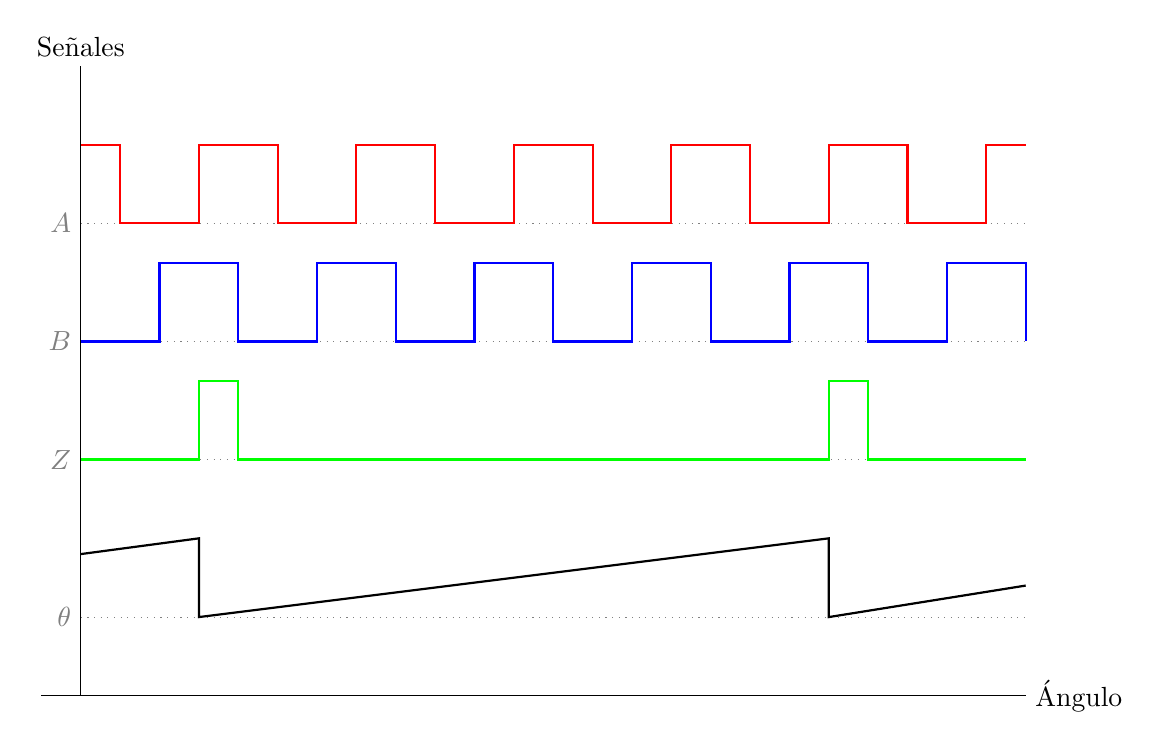
\begin{tikzpicture}[x=0.5cm,y=1cm]
		
		% Ejes y etiquetas
		\draw[-] (-1,-3) -- (24,-3) node[right] {Ángulo};
		\draw[-] (0,-3) -- (0,5) node[above] {Señales};
		
		% Señales
		\draw[dotted,gray] (0,0) node[left] {$Z$} -- (24,0);
		\draw[dotted,gray] (0,1.5) node[left] {$B$} -- (24,1.5);
		\draw[dotted,gray] (0,3) node[left] {$A$} -- (24,3);
		\draw[dotted,gray] (0,-2) node[left] {$\theta$} -- (24,-2);
		
		% Pulsos A
		\draw[thick,red] (0,4) -- (1,4) -- (1,3) -- (3,3) -- (3,4) -- (5,4) -- (5,3) -- (7,3) -- (7,4) -- (9,4) -- (9,3) -- (11,3) -- (11,4) -- (13,4) -- (13,3) -- (15,3) -- (15,4) -- (17,4) -- (17,3) -- (19,3) -- (19,4) -- (21,4) -- (21,3) -- (23,3) -- (23,4) -- (24,4);
		
		% Pulsos B
		\draw[thick,blue] (0,1.5) -- (2,1.5) -- (2,2.5) -- (4,2.5) -- (4,1.5) -- (6,1.5) -- (6,2.5) -- (8,2.5) -- (8,1.5) -- (10,1.5) -- (10,2.5) -- (12,2.5) -- (12,1.5) -- (14,1.5) -- (14,2.5) -- (16,2.5) -- (16,1.5) -- (18,1.5) -- (18,2.5) -- (20,2.5) -- (20,1.5) -- (22,1.5) -- (22,2.5) -- (24,2.5) -- (24,1.5);
		
		% Pulsos Z
		\draw[thick,green] (0,0) -- (3,0) -- (3,1) -- (4,1) -- (4,0) -- (19,0) -- (19,1) -- (20,1) -- (20,0) -- (24,0);
		
		% Diente de sierra
		\draw[thick,black] (0,-1.2) -- (3,-1) -- (3,-2) -- (19,-1) -- (19,-2) -- (24,-1.6);
		
	\end{tikzpicture}
	
	
	\caption{Señales de un \textit{encoder} incremental de 4 PPR junto al ángulo real ($\theta$) girando en sentido antihorario.}
	\label{fig:encoder_incremental}
\end{figure}


Para estimar la velocidad, dirección y posición del motor a partir del \textit{encoder} incremental, se utilizan los pulsos de los canales A y B. La dirección del movimiento se determina mirando si A está avanzada respecto a B (sentido antihorario) o viceversa (sentido horario). La velocidad se calcula midiendo el intervalo entre pulsos y la posición se determina contando (integrando) el número de pulsos desde una posición de referencia conocida.

Sin embargo, este tipo de sensor, al igual que otros, presenta un desafío: hasta que no se obtiene la señal de índice, la posición es desconocida. Una solución efectiva podría ser implementar un lazo abierto de tensión hasta obtener el pulso que marca el origen, ya que no requiere una lectura de posición previa ya que el ángulo se impone externamente. En el contexto de la tracción eléctrica, no es viable girar el motor libremente al iniciar el convertidor, ya que esto implicaría un desplazamiento involuntario del vehículo. El lazo abierto de tensión sería una solución adecuada para la aplicación específica de la Formula Student, dado que los motores están acoplados a las ruedas mediante una reductora de velocidad, con una relación de transmisión típica de alrededor de 10. Esto implica que, en el peor escenario, el motor deberá dar una vuelta mecánica completa antes de obtener un pulso de índice, lo que resulta en que la rueda gire aproximadamente una décima parte de una revolución mediante el control de lazo abierto. Tras obtener el pulso de índice, se puede operar en lazo cerrado sin mucha dificultad.

Otra posibilidad es inicializar la variable de la posición con un valor arbitrario hasta obtener el pulso de índice, aunque se desconoce si este método podría causar problemas más allá de la falta de rendimiento durante este periodo inicial.

El \textit{hardware} necesario para leer la señal del \textit{encoder} incremental puede consistir únicamente en el uso de tres comparadores analógicos. Estos comparadores se encargan de convertir las señales comúnmente diferenciales de los canales A, B y Z en señales digitales que pueden ser procesadas por el MCU del inversor. Esta interfaz también sería compatible con sensores de posición Hall, lo que brinda flexibilidad en la elección del sensor de posición para el inversor.


\subsection{Microcontrolador}

La unidad de procesamiento del convertidor es una de las piezas clave, pues será la encargada de gestionar lecturas analógicas, alarmas, comunicaciones, y por supuesto, ejecutar el control. Por ello su selección debe ser meticulosamente estudiada. En primer lugar se seleccionan unos requisitos:

\begin{itemize}
	\item \textbf{Velocidad de reloj mayor a 200 MHz}: En base a la experiencia del autor con otros inversores, el cálculo de todos los PIs, filtros, transformadas y trayectorias de control puede tomar hasta 2500 ciclos de reloj. Por lo tanto, dado que hay que ejecutar dos lazos de control para los dos motores, $\frac{2500 \cdot 2}{200 \text{ MHz}} = 25 \text{ }\text{\unit{\micro\second}} \leftrightarrow 40 \text{ kHz}$, 200 MHz es la mínima velocidad para poder conmutar a 40 kHz.
	\item \textbf{Unidad de punto flotante}: Para evitar trabajar en coma fija, lo cual puede causar muchos problemas de integración y añade una capa de complejidad innecesaria, se pone como requisito que el MCU soporte el uso de \textit{float} de forma nativa.
	\item \textbf{Dos \textit{timers} avanzados}: Son necesarios dos \textit{timers}, uno para cada inversor, con características como la salida PWM bipolar con varios canales, configuración sencilla del tiempo muerto, etc.
	\item \textbf{Lecturas analógicas}: Se necesitan al menos un par de ADCs de 12 bits suficientemente rápidos con múltiples canales cada uno, con tal de poder capturar las corrientes de fase y las tensiones de bus adecuadamente.
	\item \textbf{Interfaces de comunicación CAN, SPI, I$^2$C y USB}: Dado que se requerirá la interacción con otros dispositivos, es esencial contar con varias interfaces de comunicación. Obviamente CAN para la comunicación con el vehículo, pero también SPI/I$^2$C para utilizar memorias externas, o UART/USB como manera de conectar el inversor de forma sencilla a un ordenador.
	\item \textbf{Capacidades de depuración avanzadas}: Se requerirá de herramientas de depuración que permitan detener el código en puntos específicos, monitorizar en tiempo real el estado de las variables, etc.
	\item \textbf{Memoria \textit{flash} superior a 500 kB}: El binario de un programa muy extenso no debería pesar mucho más de 100 kB, sin embargo, si en el futuro se programa un \textit{bootloader} u otras implementaciones como tablas de búsqueda grandes, la memoria \textit{flash} debería ser el último de los problemas.
	
\end{itemize}

Teniendo en cuenta estos requisitos, se ha evaluado una variedad de familias y marcas de MCUs y DSPs, y se ha llegado a la conclusión de que el MCU STM32F777VI de la familia F7 de STMicroelectronics cumple con todos los criterios establecidos. Sus características incluyen:

\begin{itemize}
	\item Procesador ARM Cortex-M7 con FPU, funcionando a una velocidad de hasta 216 MHz.
	\item Amplio conjunto de interfaces de comunicación, incluyendo I$^2$C, USART, SPI, CAN, USB y Ethernet.
	\item 3 ADCs (24 canales máximo) de 12 bits y hasta 2.4 MSPS.
	\item 18 \textit{timers}, incluyendo \textit{timers} de 16 y 32 bits, dos \textit{timers} con PWM avanzado.
	\item Soporte para depuración mediante interfaces SWD y JTAG, incluyendo el modo de \textit{Trace Asynchronous Serial Wire}, que incorpora un pin de comunicación serie independiente de las capacidades de \textit{debug} de SWD.
	\item Hasta 2 MB de memoria \textit{flash}, SRAM de 512 Kbytes y 16 Kbytes de RAM TCM para datos críticos en tiempo real.
\end{itemize}

El STM32F777VI cumple con todos los requisitos establecidos y proporciona capacidades adicionales que pueden ser beneficiosas para el desarrollo y la operación del convertidor. Además, es el mismo microcontrolador que se usa en el resto de ECUs del monoplaza, conviertiéndose en la elección más cómoda para el futuro desarrollo.


\subsection{\textit{Software} de CAD electrónico}

El diseño de las PCBs se realizó utilizando el \textit{software} Altium Designer, una herramienta ampliamente utilizada en la industria para diseños electrónicos. El programa ofrece una amplia gama de funcionalidades que facilitan el proceso de diseño, desde la creación de esquemáticos hasta la disposición de componentes y el enrutado de pistas.

\begin{itemize}
	\item \textbf{Creación de esquemáticos:} Altium Designer proporciona un entorno intuitivo para crear el esquemático del circuito. Primero se crean los componentes usando la información de la hoja de datos para hacer un buen \textit{footprint} y símbolo, y después se incluyen los símbolos de los componentes en el esquemático y se realizan las conexiones eléctricas.
	
	\item \textbf{Diseño de PCB:} Una vez completado el esquemático, Altium Designer facilita la transferencia de diseño a la PCB. Los componentes del esquemático quedan vinculados y de forma muy sencilla se importan los cambios del esquemático a la PCB. Posteriormente se realizan las conexiones eléctricas en la PCB en un proceso conocido como enrutado.
	
	\item \textbf{Verificación de reglas:} Altium Designer permite definir y verificar reglas de diseño para garantizar que la PCB cumpla con las restricciones de los fabricantes. Esto incluye reglas de espaciado, de colisiones, etc.
	
	\item \textbf{Generación de archivos de fabricación:} Una vez completado el diseño de la PCB, Altium Designer facilita la generación de archivos necesarios para la fabricación, como los archivos \textit{Gerber}, la lista de materiales (BOM) o el archivo de taladros. Además, permite exportar un modelo 3D de la PCB con todos los componentes, lo cual facilita mucho la integración mecánica.
	
\end{itemize}

\subsection{PCB de potencia}

Esta PCB es una placa de 4 capas que integra componentes de potencia y circuitos de adquisición para el control de un solo motor eléctrico. Se requieren de dos de estas PCBs para montar el convertidor al completo.

\subsubsection{Concepto y \textit{layout}}

La PCB de potencia es el sustrato físico sobre el cual se montan y conectan los componentes de potencia. En ella están situados los semiconductores, el bus de condensadores, las medidas de tensión, corriente y temperatura, los \textit{gate drivers}, y algunos circuitos de seguridad. En la figura \ref{sketches_layout} se muestran unos bocetos iniciales que se usaron para tantear el emplazamiento de los componentes y conexiones de potencia.

\begin{figure}[H]
	\centering
	\begin{minipage}{0.35\textwidth}
		\centering
		\includegraphics[width=\textwidth]{fig/boceto5}
	\end{minipage}\hfill
	\begin{minipage}{0.55\textwidth}
		\centering
		\includegraphics[width=\textwidth]{fig/boceto6}
	\end{minipage}
	\caption{Bocetos del \textit{layout} del inversor.}
	\label{sketches_layout}
\end{figure}


\begin{figure}[H]
	\centering
	\includegraphics[width=0.7\linewidth]{fig/layout}
	\caption{\textit{Layout} de la PCB de potencia, con las zonas más importantes marcadas.}
\end{figure}

En el \textit{layout} se distinguen varias zonas. 
\begin{itemize}
	\item \textbf{Zona 1:} Conector a la PCB de control y protección de la alimentación de baja tensión.
	\item \textbf{Zona 2:} Conectores de las fases del motor y montajes mecánicos.
	\item \textbf{Zonas 3, 4 y 5:} Semiconductores, sensores de corriente, \textit{gate drivers} y \textit{snubbers} para cada fase.
	\item \textbf{Zona 6:} Bus de condensadores, conectores de alta tensión DC, circuito de descarga y sensado de tensión.
\end{itemize}

\subsubsection{Restricciones y enrutado}
Para dotar al convertidor de una alta densidad de potencia se decidió un formato de 150 mm por 200 mm, dejando espacio más que suficiente para distribuir todos los componentes de forma más o menos holgada.

Dado que esta PCB implementa partes del circuito del sistema de tracción y partes del sistema de baja tensión, se debe crear una separación física de 4 mm ya que estará acabada con un revestimiento conformal acrílico (\textit{conformal coating}), acorde con la norma \textbf{\textit{EV4.3.6}} \cite{FSG}.

Los espaciados entre conductores de la parte de alta tensión son de 3 mm, ya que la tensión que deben aislar es de 600 V. Este valor se obtiene de la norma genérica IPC-2221B \cite{IPC2221B}, que especifica una separación de $2.5+(V-500)\cdot0.005 \text{ mm} = 3 \text{ mm}$. De todas maneras, se usará un revestimiento conformal acrílico para asegurar una mejor característica dieléctrica y prevenir la aparición de arcos eléctricos.

El dimensionamiento de las pistas para la corriente que debe pasar es algo complicado, y de hecho condiciona el apilado de la PCB. Por ello, se selecciona un apilado de 4 capas de 70 micras (2 onzas por pulgada cuadrada).

\begin{figure}[H]
	\centering
	\includegraphics[width=0.7\linewidth]{fig/stackup_power}
	\caption{Apilado de la PCB de potencia.}
\end{figure}

Para dimensionar el ancho de estas pistas se ha considerado la corriente RMS de fase, ya que es la corriente máxima en toda la PCB. Después, se ha usado este ancho para todas las conexiones de potencia, aunque la corriente que vean sea menor. El cálculo se ha realizado usando la norma IPC-2152 \cite{IPC2152}, que especifica unas relaciones de capacidad de corriente respecto al incremento de temperatura y el grosor de capa. Ya que el cálculo es algo tedioso, se opta por el uso de una calculadora específica para este propósito:

\begin{figure}[H]
	\centering
	\includegraphics[width=0.7\linewidth]{fig/width}
	\caption{Cálculo del ancho de pista necesario.}
\end{figure}

El resultado es de 10 mm, lo cual es exagerado, pero sin embargo, solamente se está teniendo en cuenta una capa. Por ello, se decide enrutar las conexiones de potencia por un mínimo de 2 capas con un ancho mínimo de 5 mm. A continuación se detalla el enrutado de la conexión DC positiva de uno de los 3 módulos de medio puente.

\begin{figure}[H]
	\centering
	\begin{subfigure}{0.35\linewidth}
		\centering
		\includegraphics[width=\linewidth]{fig/ts+bot}
		\caption{Vista del enrutado de baja corriente (azul), la conexión positiva del bus de continua (naranja) y de la fase A (rosado).}
	\end{subfigure}
	\hfill
	\begin{subfigure}{0.35\linewidth}
		\centering
		\includegraphics[width=\linewidth]{fig/layout2}
		\caption{Detalle de una sección más estrecha.}
	\end{subfigure}
	\caption{Ejemplo de enrutado de la conexión DC positiva del medio puente de la fase A.}
\end{figure}

Como se puede apreciar, el espaciado que hay que dejar por aislamiento compite por espacio con el ancho de las conexiones. En la mayoría de casos se ha podido respetar el ancho mínimo de 5 mm, sin embargo, en algunas situaciones esto no es posible. Por ejemplo, lo ilustrado en la subfigura (b) muestra una estrechez de 1,5 mm, pero como esa conexión está repetida en dos capas, el ancho total es de 3 mm. Además, la conexión positiva en el semiconductor se realiza a través de dos grupos de pines, y como antes de realizar esa estrechez ya se ha conectado un grupo de pines, se puede asumir que la corriente que circula por ese trozo de cobre es la mitad que la corriente continua entera que va a recibir ese módulo, que a su vez, es aproximadamente un tercio de la corriente continua total ($\frac{1}{3}\frac{17.5 \text{ kW}}{450 \text{ V}} = 13 \text{ A}$), pasado por la calculadora, tan solo son necesarios 2,8 mm de cobre para esa corriente, lejos de los 10 mm que se han intentado mantener.

Esto es tan solo un ejemplo del análisis que se ha realizado con cualquier mínima sospecha de falta de cobre en todo el enrutado de potencia. Un camino de corriente muy estrecho podría presentar sobrecalentamiento y en casos extremos, levantamiento de la pista o plano.

Además, se han especificado el acabado y el espesor de cobre en las vías para asegurar un buen montaje de los componentes \textit{press-fit} (los conectores de potencia y los semiconductores). Se ha optado por un acabado ENIG (oro electrolítico) por ser una opción con la que se pueden hacer este tipo de conexiones, además de aguantar mucho tiempo sin oxidarse. El ancho de cobre en las vías es algo que se debe consultar directamente con el fabricante porque no todos son capaces de asegurar una tolerancia. Para saber cuánto cobre es necesario, se han consultado los documentos explicativos de Würth Elektronik (para los conectores de potencia) y de Wolfspeed (para los semiconductores).

\begin{figure}[H]
	\centering
	\includegraphics[width=0.7\linewidth]{fig/pressfit-wolfspeed-instructions}
	\caption{Requisitos para la PCB según Wolfspeed \cite{WolfspeedMountingGuide}.}
\end{figure}
\begin{figure}[H]
	\centering
	\includegraphics[width=0.7\linewidth]{fig/pressfit-wurth-instructions}
	\caption{Requisitos para la PCB según Würth Elektronik \cite{WurthRedCubeGuide}.}
\end{figure}

Ambos documentos apuntan que un acabado de estaño químico es lo ideal para realizar esta conexión, sin embargo, no se pudo conseguir un fabricante que lo pudiera realizar a un precio razonable. El grosor de cobre que se marcó como requisito al fabricante fue de 25 \unit{\micro\meter} a 50 \unit{\micro\meter}, por ser el más restrictivo de ambos.

\subsubsection{Bloques funcionales}

La PCB de potencia se divide en varios bloques funcionales, unidos en un esquemático jerárquico que además incluye la conexión entre estos bloques, algunas notas indicativas y componentes que no pertenecen a ningún bloque en específico.

\begin{figure}[H]
	\centering
	\includegraphics[width=0.8\linewidth]{fig/schPower1}
	\caption{Esquemático jerárquico de la PCB de potencia.}
\end{figure}

En el esquemático se pueden distinguir el conector a la PCB de control, la protección de alimentación de baja tensión y unas notas indicativas, así como una leyenda de colores. Se anotan también los cambios y la fecha en la que se envía a producción. Los bloques que se pueden ver incluyen:

\begin{itemize}
	
	\item \textbf{Etapa de potencia:} En este bloque aparecen los semiconductores, el bus de condensadores y una descarga pasiva.
	
	\item \textbf{Sensado de corriente:} Se incluyen los sensores de corriente y su interfaz analógica con la PCB de control.
			
	\item \textbf{\textit{Gate drivers}:} En este bloque se recogen las señales necesarias para la conmutación, así como la configuración de los \textit{gate drivers} en su conjunto. Este bloque contiene 3 subcircuitos correspondientes con cada fase. En ellos se encuentran los \textit{gate drivers} en sí, junto a su alimentación aislada, los \textit{snubbers} y la medida de temperatura.
		
	\item \textbf{DC:} Por último, hay un bloque dedicado al bus de continua, que incluye el circuito de descarga, la medida de tensión y la detección de 60 V requerida por la normativa.
\end{itemize}

\subsubsection{Circuitos importantes}

\textbf{VSI}

Ya que los módulos son estructuras \textit{half-bridge}, se deben conectar entre sí para formar la topología VSI.
\begin{figure}[H]
	\centering
	\includegraphics[width=0.7\linewidth]{fig/VSI-shc}
	\caption{Conexión de los módulos configurando un VSI.}
\end{figure}

\textbf{Protección de alimentación}

Aunque en principio es regulada, la entrada de 5 V necesita de un mínimo de protecciones sencillas para evitar retrasos ocasionados por fallos mientras se realizan pruebas. En este caso se ha usado un fusible como protección contra sobrecorriente, un diodo \textit{zener} a modo de protección contra sobretensión (hará saltar el fusible cuando la tensión de entrada supere la tensión umbral), y un diodo \textit{schottky} como protección frente a tensión inversa, ya que tiene poca caída de tensión, actúa bastante rápido y es barato.
\begin{figure}[H]
	\centering
	\includegraphics[width=0.5\linewidth]{fig/5V-sch}
	\caption{Circuito de protección de alimentación.}
\end{figure}

\newpage

\textbf{Alimentación del \textit{gate driver}}

\begin{figure}[H]
	\centering
	\includegraphics[width=0.9\linewidth]{fig/GD-supp-sch}
	\caption{Alimentación bipolar aislada del \textit{gate driver}.}
\end{figure}

En función del modelo de DC-DC específico escogido de la serie MGJ2 de Murata, se tendrá una tensión positiva y negativa diferente. La tensión positiva no es muy problemática puesto que se pueden seleccionar DC-DCs con salidas de +18 V o de +15 V, valores que encajan con los recomendados por los fabricantes de los semiconductores.

Sin embargo, ese no es el caso para las tensiones negativas, ya que el valor debería poder ajustarse para ser más versátil en el desarrollo. Por ello, se implementan reguladores lineales para ajustar $V_{\text{EE,HS}}$ y $V_{\text{EE,LS}}$ durante las pruebas para afinar el voltaje negativo necesario.

$V_{\text{EE}}$ se calcula 

\[ V_{\text{EE,LS}} = -1.186 \cdot \left(1 + \frac{R1}{R2}\right)  \text{ ,}\]

donde \( R1 + R2 \approx 100 \text{ k}\Omega \) según la hoja de datos del LDO. Para las configuraciones específicas de Leapers y Wolfspeed, los valores de las resistencias son 

\begin{itemize}
	\item Leapers: \( R1 = 36 \text{ k}\Omega \), \( R2 = 56 \text{ k}\Omega \)
	\item Wolfspeed: \( R1 = 68 \text{ k}\Omega \), \( R2 = 30 \text{ k}\Omega \)
\end{itemize}

Este proceso permite ajustar de forma precisa los voltajes negativos necesarios para el correcto funcionamiento del circuito de conmutación.


\textbf{\textit{Gate driver}}
\begin{figure}[H]
	\centering
	\includegraphics[width=0.9\linewidth]{fig/GD-sch}
	\caption{\textit{Gate driver} con medida de temperatura y \textit{snubbers}.}
\end{figure}

Uno de los componentes más importantes de todo el diseño tiene una de las implementaciones más sencillas, ya que la hoja de datos del UCC21710 proporciona mucha información útil para la aplicación final.

El \textit{gate driver} UCC21710 se implementa con varias características que lo hacen adecuado para su uso en aplicaciones de potencia. Las señales \textit{TRIP} y \textit{OK} están configuradas en \textit{open drain}, lo que permite que se paralelicen con los otros \textit{gate drivers} para facilitar su integración. La entrada \textit{IN-} no se utiliza y está conectada a tierra. El pin \textit{ENABLE} se controla desde el MCU, y cuando se fuerza un estado bajo durante más de 1 \unit{\micro\second}, se resetea la señal \textit{TRIP}. La señal \textit{TRIP} se lee como una interrupción externa desde el MCU, y sirve para detectar un error en los \textit{gate drivers} y actuar rápidamente.

Para la medición de temperatura, se utilizan los \textit{drivers} de los MOSFETS del \textit{low-side}. Estos proporcionan una corriente de salida de 200 \unit{\micro\ampere} en su salida, a través de la cual se puede interpretar la medida. Esta señal se convierte a PWM y luego a analógica mediante un filtro RC para ser recibida directamente por el ADC del MCU. 

El circuito de medición de temperatura utiliza el sensor NTC del semiconductor para obtener una lectura de tensión, la cual se convierte en una lectura de bits mediante el ADC del MCU. La relación entre la resistencia del NTC y la temperatura se modela utilizando la fórmula de Steinhart-Hart, que toma en cuenta el valor $\beta$ del NTC, la resistencia a una temperatura de referencia, y la temperatura ambiente. La fórmula utilizada es

\[
NTC = R_0 \cdot e^{\left[-\beta \cdot \left(\frac{1}{T_0} - \frac{1}{\text{T}}\right)\right]} \text{ .}
\]

El voltaje leído por el ADC se calcula
\[
V_{\text{ADC}} = V_{\text{CC,GD}} \cdot \left(\frac{-20 \cdot I_{\text{AIN}} \cdot (R_{\text{filt}} + NTC)}{100}\right) = 5 \text{ V} \cdot \left(\frac{-20 \cdot 200 \text{ }\text{\unit{\micro\ampere}} \cdot (10 \text{ k}\Omega + NTC)}{100}\right) \text{.}
\]

El circuito también incluye protección de \textit{Miller clamp} para evitar activaciones accidentales de los MOSFETs. Aunque los \textit{gate drivers} tienen un \textit{pull-down} activo, se ha implementado un \textit{pull-down} externo con $R_{\text{GS,HS}}$ y $R_{\text{GS,LS}}$. Sin embargo, la detección de sobrecorriente no está implementada en este diseño porque es posible que su implementación traiga más problemas que los que pretende solucionar.

Adicionalmente, se incluyen unos \textit{snubbers} consistentes en un RC entre \textit{drain} y \textit{source}, un condensador entre \textit{gate} y \textit{drain} y un condensador entre \textit{gate} y \textit{source}. En caso de encontrar problemas excesivos con la conmutación, pueden ayudar a amortiguar transitorios.

Cabe destacar que el enrutado de este subcircuito es especialmente crítico por los parásitos inductivos que se pueden ocasionar. En particular, la inductancia en el camino de retorno de \textit{gate-source} puede ser fatal para el comportamiento de la conmutación, razón por la cual se ha tirado un plano conectado al \textit{source} de cada MOSFET en el área donde se enruta su \textit{driver}, para minimizar el camino de retorno. En estas líneas, se ha enrutado en orden de prioridad, empezando por la conexión de las puertas de los MOSFETs a los \textit{drivers} y la alimentación aislada, y acabando con los \textit{snubbers}.

\begin{figure}[H]
	\centering
	\includegraphics[width=0.7\linewidth]{fig/invPowerRouting}
	\caption{Enrutado en la capa superior de un \textit{half-bridge}.}
\end{figure}

Debido a los parásitos que puede presentar el \textit{layout}, los MOSFETs pueden presentar un sobrepico de tensión excesivo al conmutar. La figura \ref{lc-layout} explica el circuito que pueden formar. Si la capacidad parásita es insuficiente, la inductancia parásita provocará una subamortiguación. Por ello, se ha minimizado el área que dejan estas conexiones para minimizar la inductancia parásita. Además, es importante añadir un condensador de desacoplo entre los terminales positivo y negativo de cada \textit{half-bridge}. 
\begin{figure}[H]
	\centering
	\includegraphics[width=0.5\linewidth]{fig/LC-layout}
	\caption{Circuito de parásitos en un convertidor \textit{buck} \cite{PowerElectronicCircuits2018}. Cada medio puente de un VSI actúa como un convertidor \textit{buck} cuando la corriente es positiva.}
	\label{lc-layout}
\end{figure}

\textbf{Descarga}
\begin{figure}[H]
	\centering
	\includegraphics[width=0.9\linewidth]{fig/discharge-sch}
	\caption{Circuito de descarga.}
\end{figure}

Una de las partes más importantes en cuanto a la seguridad eléctrica es la implementación del circuito de descarga. Este circuito se utiliza para descargar la energía almacenada en el bus de condensadores cuando el convertidor no está operativo. Los requisitos de la normativa son que el circuito debe ser capaz de descargar el bus de la tensión máxima hasta 60 V en menos de 5 segundos. Adicionalmente, el circuito debe ser capaz de aguantar de forma constante la tensión máxima.

Con tal de cumplir estos requisitos se ha optado por un circuito basado en un NMOS, cuya puerta se conecta al terminal positivo del bus a través de una resistencia de valor elevado y se limita la tensión con un diodo \textit{zener}. La puerta del MOSFET está controlada por un opto-acoplador de forma aislada desde el circuito de baja tensión. Mientras el bus tenga una tensión superior a 10 V (la tensión del \textit{zener}) y el opto-acoplador esté desactivado, el MOSFET quedará cerrado, conectando el banco de resistencias a los condensadores, descargándolos.

La selección de la resistencia se ha basado en minimizar el tamaño de la misma. La solución óptima se ha encontrado en utilizar un banco de 24 resistencias SMD de 470 k$\Omega$, en encapsulado 2512, que es capaz de disipar 1 W. Se conectan en paralelo para llegar al valor necesario para cumplir con el requisito de tiempo de descarga. Para el cálculo del tiempo de descarga se utiliza la siguiente expresión
\begin{equation}
	t_{\text{dis}} = R_{\text{dis}} \cdot C \cdot \ln\left(\frac{V_{\text{inicial}}}{V_{\text{final}}}\right)\text{ .}
\end{equation}

\[
t_{\text{dis}} = R_{\text{dis}} \cdot C \cdot \ln\left(\frac{V_{\text{inicial}}}{V_{\text{final}}}\right) = \left(\frac{470 \text{ k}\Omega}{24}\right) \cdot (100\text{ }\text{\unit{\micro\farad}}) \cdot \ln\left(\frac{600 \text{ V}}{60 \text{ V}}\right) = 4.509 \text{ s}
\] 

La potencia disipada en cada resistencia de descarga se calcula como

\begin{equation}
	P(R_{\text{dis}}, \text{máx}) = \frac{V_{\text{máx}}^2}{R_{\text{dis}}} \text{ .}
\end{equation}

\[
P(R_{\text{dis}}, \text{máx}) = \frac{V_{\text{máx}}^2}{R_{\text{dis}}} = \frac{(600\text{ V})^2}{470 \text{ k}\Omega} = 0.766 \text{ W} < 1 \text{ W}
\]

\textbf{Medida de corriente}

\begin{figure}[H]
	\centering
	\includegraphics[width=0.8\linewidth]{fig/Imeas-sch}
	\caption{Sensor de corriente de fase.}
\end{figure}

Uno de los componentes más críticos para asegurar el funcionamiento óptimo del inversor es la medición precisa de corriente. En inversores de bajo coste, comúnmente se emplean resistencias \textit{shunt} junto con amplificadores aislados para esta tarea. Sin embargo, esta solución puede presentar diversos desafíos de integración.

Una opción destacada para abordar esta necesidad de medición de corriente es la gama de sensores CKSR-NP de LEM. Este sensor utiliza la tecnología de transductores de corriente basados en \textit{fluxgate}. Sus características incluyen un rango de medición amplio de hasta $\pm$150 A para modelo seleccionado, junto con una alta precisión del 0.8\%. Además, su diseño compacto y montaje en PCB lo hacen ideal para aplicaciones donde se requiere una medición precisa y confiable de corriente en un espacio limitado.

Dado que el sensor tiene un rango de medida de $\pm$150 A y está alimentado a 5 V, se puede pasar por un divisor resistivo con tal de adecuar la señal de salida al rango de entrada del ADC del MCU. Adicionalmente, se puede modificar la tensión de referencia (salida a 0 A) para ajustar todavía más la medida.

\begin{figure}[H]
	\centering
	\includegraphics[width=0.5\linewidth]{fig/cksr50}
	\caption{Sensor de corriente LEM CKSR 50-NP \cite{LEMDatasheet}.}
\end{figure}

Cabe destacar que la serie CKSR-NP de LEM es compatible en especificaciones y \textit{footprint} con la serie LKSR-NP, con lo que se pueden usar indistintamente. Para el proyecto se han conseguido muestras de LKSR-NP y se compraron unos pocos CKSR-NP.

\textbf{Medida de tensión}

\begin{figure}[H]
	\centering
	\includegraphics[width=0.8\linewidth]{fig/Vmeas-sch}
	\caption{Circuito de medida y detección de tensión DC.}
\end{figure}

El sensado de la tensión es una tarea crítica en el sistema, ya que no solo es esencial para el control del motor, sino también para la detección y alerta de niveles altos de tensión. Para ambos propósitos, se emplea un divisor de tensión utilizando una serie de resistencias. 

\[ V_{\text{DC,div}} = \left(TS^+ - TS^-\right) \cdot \left( \frac{4.7 \text{ k}\Omega}{4.7 \text{ k}\Omega + 6 \cdot 68 \text{ k}\Omega} \right) \]

Sustituyendo los valores de 600 V y 60 V para TS+ y TS-, respectivamente,
\[ V_{\text{DC,div}} = \frac{600 \text{ V} \cdot 4.7 \text{ k}\Omega}{4.7 \text{ k}\Omega + 6 \cdot 68 \text{ k}\Omega} = 6.833 \text{ V} \]
\[ V_{\text{DC,div}} = \frac{60 \text{ V} \cdot 4.7 \text{ k}\Omega}{4.7 \text{ k}\Omega + 6 \cdot 68 \text{ k}\Omega} = 683 \text{ mV .} \]

El valor de potencia disipada en las resistencias de 68 k$\Omega$ se calcula 
\[ P_{\text{R68k}} = I_{\text{R4k7}}^2 \cdot 68\text{ k}\Omega = \left( \frac{V_{\text{DC,div,máx}}}{4.7\text{ k}\Omega} \right)^2 \cdot 68 \text{ k}\Omega = \left( \frac{6.833 \text{ V}}{4.7\text{ k}\Omega} \right)^2 \cdot 68 \text{ k}\Omega = 144 \text{ mW.} \]

Se elige un encapsulado 1206 para las resistencias de 68 k$\Omega$, que es capaz de disipar por lo menos 250 mW.

El amplificador aislado ISO224 se utiliza para medir la tensión en el bus de continua. Según la hoja de datos, la salida se calcula como un tercio del voltaje de entrada del divisor de tensión.
\[ (V_{\text{DC,sns+}} - V_{\text{DC,sns-}}) = \frac{1}{3} \cdot V_{\text{DC,div}} = \frac{1}{3} \cdot \left( (TS^+ - TS^-) \cdot \frac{4.7 \text{ k}\Omega}{4.7 \text{ k}\Omega + 6 \cdot 68 \text{ k}\Omega} \right) \]
\[ (V_{\text{DC,sns+}} - V_{\text{DC,sns-}}) = \frac{1}{3} \cdot 0.011388 \cdot (TS^+ - TS^-) \]
\[ (V_{\text{DC,sns+}} - V_{\text{DC,sns-}}) = \frac{1}{3} \cdot 0.011388 \cdot 600 \text{ V} = 2.278 \text{ V} \]

El amplificador aislado ISO224 es una elección eficaz para esta aplicación, ya que permite medir de manera precisa la diferencia de potencial entre los terminales, proporcionando un voltaje de salida proporcional a la tensión medida y cuadrando con el rango de adquisición del ADC. Adicionalmente, la salida es diferencial, lo que permite mayor inmunidad frente a interferencias al ser enrutada hasta la placa de control. En ella se deberá incluir un amplificador diferencial o similar para llevar la lectura al ADC.

\subsubsection{Resultado final}

Tras haber creado todos los subcircuitos, haber emplazado cada componente y enrutado cada nodo, se ha completado el diseño de la placa de potencia. La distribución de componentes permite empaquetar dos de estas placas enfrentadas de forma muy compacta, dejando el espacio justo entre medias para la inserción de la \textit{coldplate}. La placa de control se podrá conectar a las dos de potencia mediante conectores placa a placa, quedando a uno de las caras libres. Por la otra cara se deben incluir las conexiones de potencia DC y la entrada y salida de agua.

\begin{figure}[H]
	\centering
	\begin{subfigure}{0.45\linewidth}
		\centering
		\includegraphics[width=\linewidth]{fig/invPower1}
		\caption{Vista superior.}
	\end{subfigure}
	\hspace{0.05\linewidth} % Espacio horizontal entre subfiguras
	\begin{subfigure}{0.45\linewidth}
		\centering
		\includegraphics[width=\linewidth]{fig/invPower2}
		\caption{Vista inferior.}
	\end{subfigure}
	\caption{Vistas 3D de la PCB de potencia.}

\end{figure}


\begin{figure}[H]
	\centering
	\begin{subfigure}{0.45\linewidth}
		\centering
		\includegraphics[width=\linewidth]{fig/invPower3}
		\caption{Vista frontal, conexión del bus DC y \textit{coldplate}.}
	\end{subfigure}
	\hspace{0.05\linewidth} % Espacio horizontal entre subfiguras
	\begin{subfigure}{0.45\linewidth}
		\centering
		\includegraphics[width=\linewidth]{fig/invPower4}
		\caption{Vista trasera, conexión de la placa de control.}
	\end{subfigure}
	\caption{Vistas 3D del ensamblaje de dos PCBs de potencia.}
	
\end{figure}


\subsection{PCB de control}

\subsubsection{Concepto y \textit{layout}}

En esta placa se alojará el microcontrolador con todos los componentes necesarios para interactuar con las placas de potencia y el exterior. Dado que el esfuerzo de integración es mucho menor, las restricciones mecánicas y la facilidad de montaje son las que rigen el concepto. Por ello no se han tenido muchos miramientos para la disposición de los componentes, y simplemente se ha puesto atención en utilizar muchas simetrías para hacer que los circuitos repetidos para los dos motores/inversores sean exactamente iguales.

\begin{figure}[H]
	\centering
	\includegraphics[width=0.8\linewidth]{fig/controlLayout}
	\caption{\textit{Layout} de la PCB de control.}
\end{figure}

Como se puede observar, el microcontrolador es la pieza central y está orientado a 45 grados para que los pines se puedan enrutar de forma óptima hacia los extremos de la placa. Ambos lados de la placa son simétricos a excepción de los componentes que no están duplicados por el control dual.

\subsubsection{Restricciones y enrutado}

Se ha mencionado ya que esta placa no tiene muchas restricciones más allá de las mecánicas, lo cual ha permitido crearla en un formato de 150 mm por 40 mm, encajando perfectamente en ángulo recto con las placas de potencia en el espacio que dejan entre medias. 

El apilado escogido es un estándar de 4 capas, con 35 micras de espesor en todas las capas (1 onza por pulgada cuadrada). Para hacer la placa incluso más barata, se puede fabricar con 17 micras en las capas internas (0.5 onzas por pulgada cuadrada). Esto asegura una producción económica, y la posibilidad de crear planos de referencia y alimentación en las capas internas.

\begin{figure}[H]
	\centering
	\includegraphics[width=0.7\linewidth]{fig/stackup_control}
	\caption{Apilado de la PCB de control.}
\end{figure}

Dado que no hay grandes magnitudes eléctricas, el enrutado se ha centrado en minimizar el área de los caminos de corriente entre cada señal y la masa de la placa. Utilizando polígonos conectados a la masa en múltiples capas (tanto la de la propia señal como las que queden por encima o por debajo) se minimiza muchísimo este área.

También se ha procurado mantener todas las señales rápidas lo más separadas posibles para evitar el \textit{cross-talk} entre ellas, causado por el acople capacitivo que presentan dos conductores paralelos. En ocasiones no se ha podido evitar y tan solo queda confiar en el resto de buenas prácticas de enrutado.

\begin{figure}[H]
	\centering
	\includegraphics[width=0.7\linewidth]{fig/cross-talk-example}
	\caption{Ejemplo de grupo de señales que podrían presentar \textit{cross-talk}.}
\end{figure}


\subsubsection{Bloques funcionales}

La PCB de control se divide en varios bloques funcionales, que igual que la PCB de potencia, se juntan en un esquemático jerárquico. 
	
\begin{figure}[H]
	\centering
	\includegraphics[width=0.7\linewidth]{fig/schControl1}
	\caption{Esquemático jerárquico de la PCB de control.}
\end{figure}

En el esquemático se pueden apreciar el conector al vehículo, las monturas de la placa, unas notas indicativas con los cambios y una leyenda de colores. Los bloques son los siguientes:

\begin{itemize}
	\item \textbf{Alimentación}: Dado que esta placa no tiene conexión al sistema de alta tensión, se alimenta exclusivamente del sistema de baja tensión del monoplaza, cuya tensión es de entre 20 V y 30 V. Por ello se implementan distintas protecciones, un convertidor para obtener un bus de 5 V y un regulador lineal para obtener 3.3 V estables para el MCU.
	\item \textbf{MCU}: Es el bloque central, que implementa el STM32F777VI, un puerto USB, una memoria externa EEPROM y el conector de programación y depuración.
	\item \textbf{CAN}: Incluye un transceptor CAN para habilitar la comunicación con el vehículo.
	\item \textbf{Retroalimentación}: En estos bloques se integra la conexión del \textit{encoder} incremental y el \textit{front-end} analógico de la lectura de temperatura del motor.
	\item \textbf{\textit{Front-end} analógico de la placa de potencia}: Se tratan las distintas señales que provienen de las placas de potencia, adaptándolas a los rangos de tensión que admiten los ADCs del MCU.
	\item \textbf{Extras}: Tan solo se colocan unos LEDs y un par de entradas digitales para el MCU.
	
\end{itemize}

\subsubsection{Configuración de \textit{hardware} del MCU}

Con tal de asignar de forma adecuada la función de cada pin, se ha hecho uso de una herramienta proporcionada por STMicroelectronics llamada CubeMX. Este programa permite generar un código base con todos los periféricos del microcontrolador configurados según se escoja. Tiene una interfaz muy intuitiva que hace muy sencilla la implementación de \textit{hardware}, permitiendo un desarrollo muy ágil.

De esta manera, se han decidido las conexiones de la placa de control con base en las siguientes consideraciones:

\begin{itemize}
	\item \textbf{Funcionalidad del pin:} Cada pin del microcontrolador se ha configurado para cumplir una función específica de acuerdo al mapeado que tenga cada periférico, ya que normalmente un canal específico de un periférico específico solamente se puede conectar a uno o dos pines.
	
	\item \textbf{Compatibilidad con periféricos:} Se ha tenido en cuenta la compatibilidad entre los periféricos del microcontrolador y los dispositivos externos conectados a la placa de control.
	
	\item \textbf{Optimización del enrutado:} Se han escogido algunos pines a medida que se ha ido enrutando la placa, por facilitar algunas conexiones.
	
\end{itemize}

Finalmente, se logra que el esquemático y el programa CubeMX muestren la misma distribución de pines:

\begin{figure}[H]
	\centering
	\includegraphics[width=0.7\linewidth]{fig/cubeMX}
	\caption{Pantalla principal de CubeMX con todos los pines usados configurados con los periféricos adecuados.}
\end{figure}

\begin{figure}[H]
	\centering
	\includegraphics[width=0.7\linewidth]{fig/schMCU}
	\caption{Símbolo esquemático del MCU con todas las conexiones realizadas.}
\end{figure}

\subsubsection{Circuitos importantes}

\textbf{Alimentación}

Ya que se propone alimentar la placa directamente desde el sistema de baja tensión del vehículo, se debe implementar un tratamiento de esta alimentación. Se incluye protección contra descargas electrostáticas, polaridad inversa y sobrecorriente. Se implementa un DC-DC de Recom de 15 W para generar el bus principal de 5 V, sin embargo, dado a problemas de disponibilidad y ensamblaje no se ha podido probar. Además, se incluye alimentación del conector USB, y ambos buses de 5 V se pasan por un filtro Pi con frecuencia de corte $f_c = \frac{1}{2 \pi \sqrt{C \cdot L}} = \frac{1}{2 \pi \sqrt{10\text{ }\text{\unit{\micro\farad}} \cdot 47\text{ }\text{\unit{\micro\henry}}}} = 7.34 \text{ kHz}$ para evitar acoples de ruido en la alimentación. También se puede observar un regulador lineal fijo de 3.3 V para proporcionar una tensión estable al MCU, y un pequeño LED indicativo de que la alimentación está activa.

\begin{figure}[H]
	\centering
	\includegraphics[width=0.7\linewidth]{fig/schSUPPcontrol}
	\caption{Esquemático de los circuitos de alimentación de la placa de control.}
\end{figure}

\textbf{MCU}

Aunque ya se ha visto la implementación del MCU en sí, su esquemático contiene otras partes como una memoria externa, el conector USB, notas sobre qué periféricos están mapeados a qué pines y el conector de programación y depuración.

\begin{figure}[H]
	\centering
	\includegraphics[width=0.7\linewidth]{fig/schMCUcontrol}
	\caption{Esquemático de los circuitos relacionados con el MCU.}
\end{figure}
 
\textbf{CAN}

Para implementar comunicación CAN es necesario incorporar un \textit{transceiver} que pueda comunicar el MCU con un bus de CAN real. Se escoge el MCP2551 por su coste, simplicidad y robustez. Se añade también un filtro de línea consistente en un \textit{choke} para las interferencias en modo común, y algunos condensadores. Se incluye también un final de línea por si fuera necesario, y protección contra ESD. Adicionalmente, se han implementado un par de luces LED para indicar el correcto funcionamiento del envío y recepción de datos.

\begin{figure}[H]
	\centering
	\includegraphics[width=0.7\linewidth]{fig/schCANcontrol}
	\caption{Esquemático referente a la comunicación CAN.}
\end{figure}

\textbf{Retroalimentación}

Este bloque se implementa por duplicado, un bloque por cada motor que se controla. Contiene los componentes necesarios para leer su posición y temperatura.

Ya que se requiere de leer la posición con un \textit{encoder} incremental, se equipan los componentes necesarios para ello. Se usa el LM339, un comparador cuádruple con salida HiZ/GND para obtener la lectura desde una interrupción externa en el MCU. Cabe destacar que esta configuración de \textit{hardware} hace compatible este inversor con sensores de efecto Hall para la lectura de posición, aunque no se desarrollará el código que los interprete.

\begin{figure}[H]
	\centering
	\includegraphics[width=0.5\linewidth]{fig/schENCODERcontrol}
	\caption{Esquemático del \textit{front end} del \textit{encoder} incremental.}
\end{figure}

A fecha de la redacción de este trabajo todavía no se conoce el sensor de temperatura que montarán los motores, de modo que se implementa un circuito modificable para la lectura de cualquier tipo de sensor de temperatura resistivo. Aprovechando el comparador restante del LM339 se añade también una alarma configurable por \textit{hardware} para cualquier tipo de sensor.
\begin{figure}[H]
	\centering
	\includegraphics[width=0.5\linewidth]{fig/schTEMPcontrol}
	\caption{Esquemático de la lectura de temperatura del motor y alarma arbitraria.}
\end{figure}

Por último, se añade un conector para el sensor que incluye también una alimentación de 5 V, el sensor de temperatura y el sensor arbitrario junto con unas notas sobre la implementación.
\begin{figure}[H]
	\centering
	\includegraphics[width=0.5\linewidth]{fig/schFDBcontrol}
	\caption{Esquemático del conector del sensor de posición y notas.}
\end{figure}

\textbf{\textit{Front end} de la placa de potencia}

Este bloque se implementa por duplicado, un bloque por cada placa de potencia que tiene el inversor.

\begin{figure}[H]
	\centering
	\includegraphics[width=0.7\linewidth]{fig/schPOWERAFEcontrol}
	\caption{Esquemático del \textit{front end} de la placa de potencia.}
\end{figure}


En primer lugar, \textit{ENABLE} es una salida directa del MCU, y se ha comprobado que el UCC21710 es capaz de detectarla a 3.3V, igual que los PWMs. De manera similar, \textit{TRIP} se lee a 5 V y utiliza un GPIO tolerante a 5 V en el MCU.

Para que el ADC del MCU reciba correctamente todas las señales analógicas, se deben tratar adecuadamente. Hay tres grupos de señales analógicas en cada placa de potencia: las corrientes de fase, la tensión DC y la temperatura de los semiconductores.

\textit{Corrientes de Fase}

Como se ha visto en el apartado de la placa de potencia, se utilizan sensores referenciados a 5 V, y por tanto, sus señales podrían exceder el rango de 3.3 V del ADC. Por ello se implementa un simple divisor de tensión. La combinación de resistencias se puede ajustar para aumentar el rango de medición a costa de una menor resolución. 

El \textit{offset} de la corriente en bits se calcula
\[ \text{\textit{offset}}_i = \left(\frac{10 \text{ k}\Omega}{3.3\text{ k}\Omega+10\text{ k}\Omega}\right) \cdot 2.5 \text{ V} \cdot \frac{2^{12} \text{ bits}}{3.3\text{ V}} = 2333 \text{ bits ,} \]

y la ganancia de la medida de corriente
\[ \text{\textit{gain}}_i = \frac{\left(\frac{10\text{ k}\Omega}{3.3\text{ k}\Omega+10\text{ k}\Omega}\right)}{12.5 \text{ mV/A} \cdot \left(\frac{2^{12} \text{ bits}}{3.3\text{ V}}\right)} = 0.0484609962 \text{ A/bit .} \]

La corriente máxima que se puede medir es
\[ \pm 0.0484609962 \text{ A/bit} \cdot \frac{2^{12} \text{ bits}}{2} = \pm 99 \text{ A .} \]

Para los ensayos se instalaron resistencias de $4.7$ k$\Omega$ en vez de $3.3$ k$\Omega$ y se calcularon de nuevo los parámetros para la lectura correcta.

\textit{Tensión de Bus}

Dado que el amplificador aislado utilizado saca una señal diferencial, se debe convertir a \textit{single-ended} usando un amplificador diferencial integrado. 

Puesto que el modelo escogido presentaría una pequeña zona muerta, se debe añadir un \textit{offset} de muy pocos milivoltios. 

No existen referencias de tensión de tan poco nivel, así que se usa un divisor resistivo de valores bajos, a sabiendas de que esta decisión causa error en la medida. 

El \textit{offset} de la medida de tensión se calcula
\[ \text{\textit{offset}}_v = V_{ref} \cdot \frac{2^{12} \text{ bits}}{3.3\text{ V}} = 129 \text{ bits,} \]

y la ganancia de la medida de tensión en voltios por bit se calcula
\[ \text{\textit{gain}}_v = \frac{1}{\left(\frac{1}{3} \cdot 0.011388 \text{ V/V} \cdot \left(\frac{2^{12} \text{ bits}}{3.3\text{ V}}\right)\right)} = 0.212240269 \text{ V/bit.} \]

La tensión máxima que se puede medir es
\[ 0.212240269 \text{ V/bit} \cdot 2^{12} \text{ bits} = 869.34 \text{ V .} \]

\textit{Temperaturas de los semiconductores}

Sería poco práctico leer las tres temperaturas de cada inversor ya que ocuparían muchos pines del MCU. Por ello, se añaden unas pequeñas resistencias, dos de las cuales no se montan, lo cual permite escoger una de las tres medidas de temperatura. Las temperaturas de los inversores deben calcularse con una \textit{lookup table} para ahorrar tiempo de computación. Como se ha visto, la señal que sale del UCC21710 es una señal pulsada que puede leerse directamente como una entrada PWM o pasar a través de un filtro RC en la placa de potencia para convertirla en una señal analógica. Esta placa pretende leerla con el ADC.

La lectura en sí misma está en la parte de alta tensión de la placa de potencia y se conecta al pin AIN de UCC21710. Basándose en el voltaje leído, se calcula el ciclo de trabajo (D) de la salida analógica aislada de UCC21710 utilizando la relación proporcionada por el fabricante \cite{UCC21710}.

\[ D = -20 \cdot V_{AIN} + 100 .\] 

Si se filtra, el voltaje en leído por el ADC del MCU se calcula
\[ V_{Tinv} = VCC_{GD} \cdot \frac{D}{100} = 5V \cdot \left(-20 \cdot V_{AIN} + 100\right)/100 .\]


\textbf{Extras}

En este bloque aparecen tres LEDs informativos controlados por el MCU, un interruptor para cambiar la dirección de giro de los motores, y una lectura de la cadena de seguridad.

\begin{figure}[H]
	\centering
	\includegraphics[width=0.7\linewidth]{fig/schEXTRAScontrol}
	\caption{Esquemático de extras.}
\end{figure}


\subsubsection{Resultado final}
Después de diseñar todos los circuitos, emplazado todos los componentes y enrutado todos los nodos, se completa el diseño de la placa de control.


\begin{figure}[H]
	\centering
	\begin{subfigure}{0.45\linewidth}
		\centering
		\includegraphics[width=\linewidth]{fig/invControl1}
		\caption{Vista superior.}
	\end{subfigure}
	\hspace{0.05\linewidth} % Espacio horizontal entre subfiguras
	\begin{subfigure}{0.45\linewidth}
		\centering
		\includegraphics[width=\linewidth]{fig/invControl2}
		\caption{Vista inferior.}
	\end{subfigure}
	\caption{Vistas 3D de la PCB de control.}
	
\end{figure}

\subsection{Ensamblaje del convertidor}

El ensamblaje del convertidor se realizó siguiendo un proceso meticuloso para garantizar la correcta integración de todos los componentes del mismo. Se utilizó un enfoque basado en diseño asistido por computadora (CAD) para planificar y visualizar el montaje antes de la construcción física. Durante el diseño de las PCBs se fue comprobando mediante CAD que no existían colisiones y que el convertidor se podía montar, atendiendo a razones como el acceso de herramientas.

\subsubsection{Diseño en CAD}

Se utilizó Solidworks para crear un modelo tridimensional detallado del convertidor. Se empezó por importar los archivos de ambas PCBs generados por Altium.

\begin{figure}[H]
	\centering
	\includegraphics[width=0.7\linewidth]{fig/assembly1}
	\caption{Ensamblaje de la placa de control con las dos placas de potencia.}
\end{figure}

A este ensamblaje se le añadieron unas pletinas para conectar entre sí los buses de continua, ya que van conectados a la misma batería. Además, se planteó un concepto de \textit{coldplate} atendiendo únicamente a las restricciones mecánicas. Este pre-diseño no fue estudiado ni simulado, simplemente marca una primera referencia para desarrollar la \textit{coldplate} en el futuro. También se incluyó la tornillería necesaria para el montaje.

\begin{figure}[H]
	\centering
	\includegraphics[width=0.7\linewidth]{fig/assembly2}
	\caption{Ensamblaje con las pletinas, concepto de \textit{coldplate} y tornillería.}
\end{figure}

\subsubsection{Ensamblaje real}

Como se discutirá en el capítulo de resultados, el convertidor fue montado poco a poco para validar sección a sección. Se soldaron los componentes manualmente con un lápiz de soldadura e hilo de estaño. Ocasionalmente se usó una pistola de calor para extraer componentes con conexiones con mucha masa térmica.

\begin{figure}[H]
	\centering
	\includegraphics[width=0.5\linewidth]{fig/assembly3}
	\caption{Soldadura manual con hilo de estaño.}
\end{figure}

Se montó una PCB de control y dos de potencia. Aprovechando que se dispone de los dos semiconductores seleccionados, se montó una placa de potencia con cada uno. A parte de los semiconductores, a penas hay que cambiar el valor de un par de resistencias.

Para montar los componentes \textit{press-fit} se usó un tornillo de banco y un utillaje que permita apretar los componentes. Cabe destacar que se priorizó el montaje de los componentes con este tipo de conexión puesto que al realizar el proceso se generan flexiones en la placa que podrían dañar componentes como los condensadores cerámicos.

El caso de los conectores de potencia fue sencillo puesto que no son muchos pines y se pudo insertar fácilmente usando herramientas comunes. Para los semiconductores sin embargo, se tuvo que imprimir un utillaje personalizado para evitar colisiones con otros componentes.

\begin{figure}[H]
	\centering
	\includegraphics[width=0.7\linewidth]{fig/assembly4}
	\caption{Placa lista para el montaje de un componente \textit{press-fit} con un utillaje personalizado.}
\end{figure}

\begin{figure}[H]
	\centering
	\includegraphics[width=0.7\linewidth]{fig/tornilloBanco}
	\caption{Prensado del componente usando un tornillo de banco.}
\end{figure}

\begin{figure}[H]
	\centering
	\includegraphics[width=0.7\linewidth]{fig/assembly5}
	\caption{Resultado de la inserción del componente.}
\end{figure}


\begin{figure}[H]
	\centering
	\includegraphics[width=0.7\linewidth]{fig/assembly8}
	\caption{Cara trasera de la PCB de potencia (variante Wolfspeed) montada.}
\end{figure}


\begin{figure}[H]
	\centering
	\includegraphics[width=0.5\linewidth]{fig/assembly9}
	\caption{PCB de control montada.}
\end{figure}


Tras montar todos los componentes de todas las placas se procedió a ensamblarlas. A fecha de cuando se tomaron las siguientes imágenes no se dispuso de las pletinas.

\begin{figure}[H]
	\centering
	\includegraphics[width=0.7\linewidth]{fig/assembly6}
	\caption{Placa de control y placa de potencia (variante Wolfspeed).}
\end{figure}


\begin{figure}[H]
	\centering
	\includegraphics[width=0.5\linewidth]{fig/assembly7}
	\caption{Vista en la que se aprecian ambas placas de potencia con sus respectivos semiconductores, dejando el espacio para una \textit{coldplate}.}
\end{figure}


\newpage
\section{\textit{Firmware}}

\subsection{Desarrollo del \textit{firmware}}
El \textit{firmware} de un proyecto como este no se puede desarrollar al estilo \textit{maker}, de manera informal o improvisada. Requiere un enfoque metodológico y estructurado para garantizar la estabilidad, la eficiencia y la continuidad del proyecto. Es fundamental seguir prácticas de desarrollo de \textit{software} bien establecidas, como el diseño modular, la documentación detallada del código y la gestión de versiones. Además, el cumplimiento de estándares de codificación y la realización de análisis estáticos son pasos críticos para garantizar la calidad y la seguridad del \textit{firmware}. Este enfoque profesional y riguroso es esencial para crear una base de código ampliable, portable y eficiente.

\subsubsection{Herramientas utilizadas}

\textbf{Análisis estático: Cppcheck}

Cppcheck es una herramienta de análisis estático de código C/C++ que se utiliza para detectar errores y problemas potenciales en el código. Realiza un escaneo exhaustivo del código para identificar posibles problemas como fugas de memoria, uso incorrecto de punteros, variables no inicializadas y otros errores comunes de programación. La integración de Cppcheck en el flujo de trabajo de desarrollo ayuda a identificar y corregir estos problemas en una etapa temprana del proceso de desarrollo, lo que contribuye a mejorar la calidad y fiabilidad del \textit{firmware}.
\begin{figure}[H]
	\centering
	\includegraphics[width=0.7\linewidth]{fig/cppCheck}
	\caption{Cppcheck detectando un potencial problema.}
\end{figure}

\textbf{Documentación del código: Doxygen}

Doxygen es una herramienta de generación de documentación que se utiliza para crear documentación automática a partir del mismo código. Permite documentar el código usando comentarios especiales incrustados en el código mismo, utilizando una sintaxis sencilla y clara. Doxygen procesa estos comentarios para generar documentación en varios formatos, incluyendo HTML (como una pequeña web), y PDF (para una documentación más tradicional). Esta documentación incluye detalles sobre la estructura del código, la descripción de las funciones y variables, así como relaciones y dependencias entre diferentes partes del código. La generación automática de documentación con Doxygen facilita la comprensión y el mantenimiento del código, y proporciona una referencia útil para futuros desarrolladores.

\begin{figure}[H]
	\centering
	\includegraphics[width=0.7\linewidth]{fig/doxyhtml}
	\caption{Documentación del código en formato HTML generada automáticamente por Doxygen.}
	\label{fig:doxyhtml}
\end{figure}


\subsubsection{Plataforma de desarrollo}
Para el desarrollo del \textit{firmware}, se emplea STM32CubeIDE de STMicroelectronics, una plataforma de desarrollo integrado (IDE) basada en Eclipse y diseñada específicamente para trabajar con microcontroladores STM32. CubeIDE proporciona un entorno de desarrollo completo que incluye un editor de código, un compilador, un depurador y otras herramientas útiles para la programación de microcontroladores STM32. Además, integra STM32CubeMX, que facilita la configuración de periféricos y la generación de código inicial mediante una interfaz gráfica intuitiva.

\begin{figure}[H]
	\centering
	\includegraphics[width=0.7\linewidth]{fig/cubeide_code}
	\caption{STM32CubeIDE en la perspectiva de código.}
\end{figure}


El uso de CubeIDE simplifica el proceso de desarrollo de \textit{firmware} para microcontroladores STM32, ofreciendo características como autocompletado de código, resaltado de sintaxis, depuración paso a paso y visualización de variables en tiempo real.



\subsubsection{Lenguaje de programación}

El lenguaje de programación seleccionado para desarrollar el \textit{firmware} de este proyecto es C. Esta elección se basa en varias consideraciones relacionadas con la naturaleza de la aplicación embebida en un microcontrolador STM32.

En primer lugar, el lenguaje C es ampliamente compatible y soportado por la mayoría de los microcontroladores, incluidos los STM32. La vasta cantidad de recursos, bibliotecas y herramientas disponibles para el desarrollo en C facilita la implementación de funcionalidades complejas y la integración con el \textit{hardware} específico del microcontrolador.

Además, el lenguaje C es altamente eficiente en términos de uso de recursos de memoria y velocidad de ejecución, lo cual es crucial en aplicaciones embebidas donde se deben cumplir estrictas restricciones de recursos.

Se reconoce que usar C++ podría tener beneficios en la legibilidad y la modularidad por tratarse de un lenguaje orientado a objetos. Sin embargo, las ventajas de usar C son demasiadas como para considerar escribir el código en C++.

\subsubsection{Estilo de programación}

Para mantener un código claro y coherente, se seguirán las siguientes convenciones de nomenclatura y estilo de programación:

\begin{enumerate}
	\item \textbf{Convenciones generales:}
	\begin{itemize}
		\item Se usará el inglés como idioma a la hora de programar para facilitar el entendimiento.
	\end{itemize}
	\item \textbf{Convenciones de nomenclatura para variables/estructuras/enumeraciones:}
	\begin{itemize}
		\item Se utilizará \texttt{camelCase} para los nombres de variables y la declaración de estructuras/enumeraciones.
		\item Se utilizará \texttt{PascalCase} para la definición de estructuras/enumeraciones.
		\item Se emplearán nombres descriptivos que indiquen claramente el propósito de la variable.
		\item Se agregarán extensiones \texttt{\_left} y \texttt{\_right} a las variables que representen componentes del inversor izquierdo y derecho, respectivamente.
		\item Se evitará añadir más extensiones con guión bajo.
		\item Las constantes se nombrarán en MAYÚSCULAS.
	\end{itemize}
	

	\textbf{Ejemplo:}
	\begin{itemize}
		\item Para el \textit{offset} y el \textit{slope} del ADC:
		\begin{lstlisting}[language=C, basicstyle=\small\ttfamily, frame=none]
#define CURRENT_SLOPE  117.57704f  /**< [A/V] ((4.7+10)/10) * (1 / (12.5 mV / A)) */
#define CURRENT_OFFSET 1.70068027211f /**< [V] (10/(4.7+10))* 2.5 V */

		\end{lstlisting}
		\item Para la referencia de par:
		\begin{lstlisting}[language=C, basicstyle=\small\ttfamily, frame=none]
torqueRef_left
torqueRef_right
		\end{lstlisting}
		\item Para la definición y declaración de la estructura \texttt{Encoder}:
		\begin{lstlisting}[language=C, basicstyle=\small\ttfamily, frame=none]
typedef struct {} Encoder; // Encoder struct definition
Encoder encoder_left; // Declaration of encoder_left
		\end{lstlisting}
	\end{itemize}


	\item \textbf{Convenciones de nomenclatura para funciones:}
	\begin{itemize}
		\item Se utilizará \texttt{snake\_case} para los nombres de funciones.
		\item Se emplearán nombres descriptivos que indiquen claramente el propósito de la función, incluso si parecen demasiado largos.
		\item El nombre de todas las funciones debe empezar por un verbo.
	\end{itemize}
	\textbf{Ejemplo:}
	\begin{itemize}
		\item \texttt{initialize\_inverter()}
		\item \texttt{limit\_torque\_to\_prevent\_overspeed()}
		\item \texttt{handle\_direction()}
		
	\end{itemize}
	\item \textbf{Convenciones de nomenclatura para archivos:}
	\begin{itemize}
		\item Los pares de archivos .c/.h desarrollados se nombrarán en MAYÚSCULAS, facilitando su distinción de los archivos generados automáticamente.
	\end{itemize}
	\textbf{Ejemplo:}
	\begin{itemize}
		\item \texttt{MEASUREMENTS.c/.h} $\rightarrow$ Desarrollado
		\item \texttt{adc.c/.h} $\rightarrow$ Generado automáticamente
	\end{itemize}
	\item \textbf{Convenciones para abreviaturas:}
	\begin{itemize}
		\item Se utilizarán abreviaciones comunes solo cuando sean ampliamente entendidas dentro del contexto del proyecto.
		\item Se evitarán abreviaciones ambiguas o poco claras.
	\end{itemize}
	\textbf{Ejemplo:}
	\begin{itemize}
		\item \texttt{ADC} (Convertidor Analógico-Digital)
		\item \texttt{FSM} (Máquina de Estados Finitos)
		\item \texttt{LUT} (Tabla de Búsqueda)
	\end{itemize}
	\item \textbf{Comentarios:}
	\begin{itemize}
		\item Cada archivo y función debe ir precedido por un comentario estilo Doxygen que explique claramente su propósito.
	\end{itemize}
	\textbf{Ejemplo:}
	
	\begin{adjustbox}{max width=\textwidth}
	\begin{lstlisting}[language=C, basicstyle=\ttfamily\small, breaklines=true, frame=single]
				
/**
* @brief Computes d-q currents from current measurements and electrical angle.
*
* This function computes the d-q currents from phase currents (ABC), theta_e, and stores
* the results in the provided pointers.
*
* @param[in] ia Phase A current in A.
* @param[in] ib Phase B current in A.
* @param[in] ic Phase C current in A.
* @param[in] sinTheta_e Electrical angle sine (-1..1)
* @param[in] cosTheta_e Electrical angle cosine (-1..1)
* @param[out] idMeas Pointer to store the d-axis current.
* @param[out] iqMeas Pointer to store the q-axis current.
*/
void get_idiq(float ia, float ib, float ic, float sinTheta_e, float cosTheta_e, float *idMeas, float *iqMeas);

	\end{lstlisting}
\end{adjustbox}
\end{enumerate}



\subsection{Arquitectura del \textit{firmware}}

Para abordar fácilmente el manejo de los dos inversores de forma independiente, se han escrito varios módulos de código que se van reutilizando para evitar repetir código.

\subsubsection{\texttt{INVERTER.c/.h}}

El archivo \texttt{INVERTER.c} y su correspondiente encabezado \texttt{INVERTER.h} constituyen la implementación y la interfaz de la estructura de datos y las funciones asociadas a un inversor.

La principal funcionalidad de estos archivos es proporcionar una interfaz cohesiva y modular para la gestión de los inversores. La estructura \texttt{InverterStruct} definida en \texttt{INVERTER.h} encapsula todos los elementos necesarios para el funcionamiento de un inversor, incluyendo periféricos, estados de operación, estructuras de datos para mediciones y referencias y lazos de control, entre otros. Esta encapsulación permite una gestión eficiente y organizada de la complejidad asociada al control de los dos inversores. Si el código estuviera escrito en un lenguaje como C++ se podría crear una clase en vez de una estructura, pero al estar programado en C, solamente se han podido mantener las buenas prácticas de la programación orientada a objetos.

Un aspecto destacado de la implementación es la escritura de código modular y reutilizable, por ejemplo, las funciones se implementan de manera independiente de la configuración específica del \textit{hardware} del inversor. Se generan dos estructuras globales \texttt{InverterStruct} independientes, \texttt{inverter\_left} e \texttt{inverter\_right}, para controlar cada uno de los inversores de forma independiente. Esta estrategia permite un control simultáneo de ambos inversores sin repetir ni una línea de código.

\subsubsection{\texttt{MOTOR.c/.h}}

El archivo \texttt{MOTOR.c} y su correspondiente encabezado \texttt{MOTOR.h} constituyen la implementación y la interfaz de las funciones y estructuras asociadas a los parámetros y constantes del motor.

La funcionalidad principal de estos archivos es proporcionar una interfaz modular para la gestión de los parámetros del motor. La estructura \texttt{MotorParameters}, definida en \texttt{MOTOR.h}, encapsula todos los parámetros de un motor eléctrico.

Un aspecto importante de la implementación es la inclusión de una estructura adicional, \texttt{MotorConstants}, dentro de \texttt{MotorParameters}, que almacena las constantes precalculadas relacionadas con el motor. Estas constantes se calculan en la función \texttt{precalculate\_motor\_constants()} y se utilizan en el cálculo de trayectorias para ahorrar algo de tiempo de ejecución.

Además, se proporciona una función de verificación de parámetros, \texttt{check\_motor\_parameters()}, que evalúa los valores de los parámetros del motor y realiza ajustes si se detectan errores o valores fuera de los límites especificados. Esta función garantiza que los parámetros del motor estén dentro de rangos seguros.

\subsubsection{\texttt{FSM.c/.h}}

El archivo \texttt{FSM.c} y su encabezado correspondiente \texttt{FSM.h} contienen la implementación y la interfaz de la Máquina de Estados Finitos (FSM) para controlar el inversor. La FSM gestiona el funcionamiento de un inversor a través de la ejecución de diferentes estados. Cada estado representa una etapa específica en el ciclo de funcionamiento del inversor y está asociado con un conjunto definido de acciones y condiciones de transición. El archivo \texttt{FSM.c} implementa funciones para gestionar cada estado. 

Los cuatro estados implementados son:

\begin{itemize}
	\item \textbf{Inicio (\texttt{Startup})}: En este estado, se realizan las acciones de inicialización del inversor, como la configuración de periféricos y la detección de errores durante el arranque.
	\item \textbf{Reposo (\texttt{Idle})}: El inversor está inactivo y espera órdenes para iniciar o detecta condiciones de error.
	\item \textbf{Funcionamiento (\texttt{Running})}: El inversor está en pleno funcionamiento y se ejecuta el bucle de control principal.
	\item \textbf{Error (\texttt{Fault})}: Se gestionan las acciones para detener el inversor y manejar las condiciones de error.
\end{itemize}

En cada estado, se describen las acciones realizadas y las condiciones que pueden provocar una transición a otro estado, como la detección de errores o cambios en las condiciones de funcionamiento del inversor.

\begin{figure}[H]
	\centering
	\begin{tikzpicture}[node distance=4cm,every node/.append style={fill=white}]
		% Define the states
		\node[state, initial] (startup) {$Startup$};
		\node[state, right=of startup] (idle) {$Idle$};
		\node[state, below right=2cm and 5cm of idle] (running) {$Running$};
		\node[state, below=of startup, draw=red, text=red] (fault) {$Fault$};
		% Draw the transitions
		\draw[-Stealth] (startup) edge[bend left] node[pos=0.25] {1} (idle)
		(idle) edge[loop above] node[pos=0.5, above] {Idle} (idle)
		(idle) edge[bend left] node[pos=0.25] {enable == 1} (running)
		(running) edge[loop below] node[pos=0.5, below] {Running} (running)
		(running) edge[bend left] node[pos=0.25] {enable == 0} (idle)
		(fault) edge[bend left] node[align=center, pos=0.25] {error == 0 AND\\enable == 0} (idle);

		
		% Redefine the transitions to "Fault" state in red
		\draw[-Stealth, red] (idle) edge[bend left] node[pos=0.25, text=red] {error != 0} (fault)
		(running) edge[bend left] node[pos=0.25, text=red] {error != 0} (fault)
		(fault) edge[loop below] node[align=center, pos=0.5, below, text=red] {error != 0 OR\\enable == 1} (fault)
		(startup) edge[bend right] node[pos=0.25, text=red] {error != 0} (fault);
	\end{tikzpicture}
	\caption{Diagrama de estados de la FSM para el control de un inversor.}
\end{figure}

\subsubsection{\texttt{ERRORS.c/.h}}

Los archivos \texttt{ERRORS.c} y su correspondiente encabezado \texttt{ERRORS.h} proporcionan las funciones necesarias para establecer, leer y eliminar errores del sistema.

En este archivo, se define una enumeración llamada \texttt{InverterError} que representa los diferentes estados de error del inversor. Cada error se representa como un bit en un número entero sin signo de 32 bits (\texttt{uint32\_t}).


\begin{table}[H]
	\centering
	\begin{tabular}{|p{2cm}|*{10}{p{0.5cm}|}}
		\hline
		Posición & 0 & 1 & 2 & 3 & 4 & 5 & 6 & 7 & 8 & 9 \\
		\hline
		Código & \rotatebox{90}{POWER\_FAULT} & \rotatebox{90}{OVERTEMPERATURE\_INV} & \rotatebox{90}{OVERVOLTAGE} & \rotatebox{90}{OVERCURRENT} & \rotatebox{90}{OVERSPEED} & \rotatebox{90}{UNDERVOLTAGE} & \rotatebox{90}{CONTROL\_FAULT} & \rotatebox{90}{WARNING} & \rotatebox{90}{OVERTEMPERATURE\_MOT } & \rotatebox{90}{FEEDBACK\_FAULT} \\
		\hline
		Ejemplo & 0 & 0 & 0 & 0 & 0 & 0 & 1 & 0 & 0 & 1 \\
		\hline
	\end{tabular}
	\caption{Mapa de errores.}
\end{table}

Por ejemplo, si los bits 0 y 3 están establecidos (valor binario 00 0000 1001 o valor decimal 9), significa que se ha producido un error en la etapa de potencia y otro de sobrecorriente.


En \texttt{ERRORS.c}, se implementan las siguientes funciones:

\begin{itemize}
	\item \texttt{set\_error}: Esta función establece un error específico en el campo de errores de una estructura de datos. Toma como argumentos un puntero a la estructura de datos y el error a establecer.
	\item \texttt{clear\_error}: Esta función elimina un error específico del campo de errores de una estructura de datos. Toma como argumentos un puntero a la estructura de datos y el error a eliminar.
	\item \texttt{is\_error\_set}: Esta función verifica si un error específico está establecido en el campo de errores de una estructura de datos. Toma como argumentos un puntero a la estructura de datos y el error a verificar.
\end{itemize}

Estas funciones proporcionan una interfaz para manejar los errores del sistema de manera eficiente y modular. Al representar los errores como bits en un entero sin signo, se optimiza el uso de memoria y se facilita la manipulación y el análisis de los errores individuales.


\subsubsection{\texttt{MEASUREMENTS.c/.h}}

Los archivos \texttt{MEASUREMENTS.c} y su encabezado correspondiente \texttt{MEASUREMENTS.h} contienen la implementación y la interfaz para manejar las mediciones en el sistema.

En \texttt{MEASUREMENTS.h}, se definen algunas constantes relacionadas con ganancias y desplazamientos para corriente y voltaje, así como umbrales de falla para diversas condiciones del sistema. Además, se declaran las estructuras de datos necesarias para almacenar las mediciones de los sensores y los valores de retroalimentación.

Las estructuras definidas son:

\begin{itemize}
	\item \texttt{Encoder}: Estructura para la lectura del \textit{encoder}, que almacena los valores de los canales A, B y Z, así como la velocidad angular eléctrica y la posición del rotor eléctrico.
	\item \texttt{Analog}: Estructura para las mediciones de los sensores analógicos de cada inversor, es decir, las corrientes de fase y la tensión del bus DC.
	\item \texttt{Feedback}: Estructura para los valores de retroalimentación, que contiene corrientes $d-q$, par calculado y velocidad medida.
\end{itemize}

En \texttt{MEASUREMENTS.c}, se implementan las funciones para manejar las mediciones, como la conversión de lecturas de ADC a medidas físicas, el cálculo de corrientes $d-q$ a partir de las mediciones de corriente de fase y el ángulo eléctrico, y la calibración de los \textit{offsets} de los sensores de corriente.

\subsubsection{\texttt{REFERENCE.c/.h}}

Los archivos \texttt{REFERENCE.c} y su encabezado correspondiente \texttt{REFERENCE.h} proporcionan funciones para manejar la consigna de par de cada motor. En \texttt{REFERENCE.h}, se define una estructura de datos llamada \texttt{Reference}, que contiene los valores de consigna para las corrientes $d-q$ y el par. 

Las funciones principales implementadas en \texttt{REFERENCE.c} son:

\begin{itemize}
	\item \texttt{set\_torque\_direction}: Esta función ajusta la dirección del par en función de la dirección deseada del motor.
	\item \texttt{saturate\_symmetric}: Esta función satura simétricamente un valor de referencia en función del valor máximo permitido.
	\item \texttt{limit\_torque\_to\_prevent\_overspeed}: Esta función actúa como una saturación de par, reduciendo el par para limitar la velocidad máxima del motor.
	\item \texttt{handle\_torqueRef}: Esta función llama a las anteriores y las encadena para gestionar adecuadamente la consigna de par.
\end{itemize}

Además, se crea un \textit{derating} lineal para la corriente, que limita el valor máximo de la consigna:

\begin{itemize}
	\item \texttt{calculate\_derated\_current}: Calcula la corriente máxima basada en umbrales de temperatura.
	\item \texttt{derate\_current\_reference}: Limita la referencia de corriente basándose en las temperaturas del motor y del inversor.
\end{itemize}

\begin{figure}[H]
	\centering
	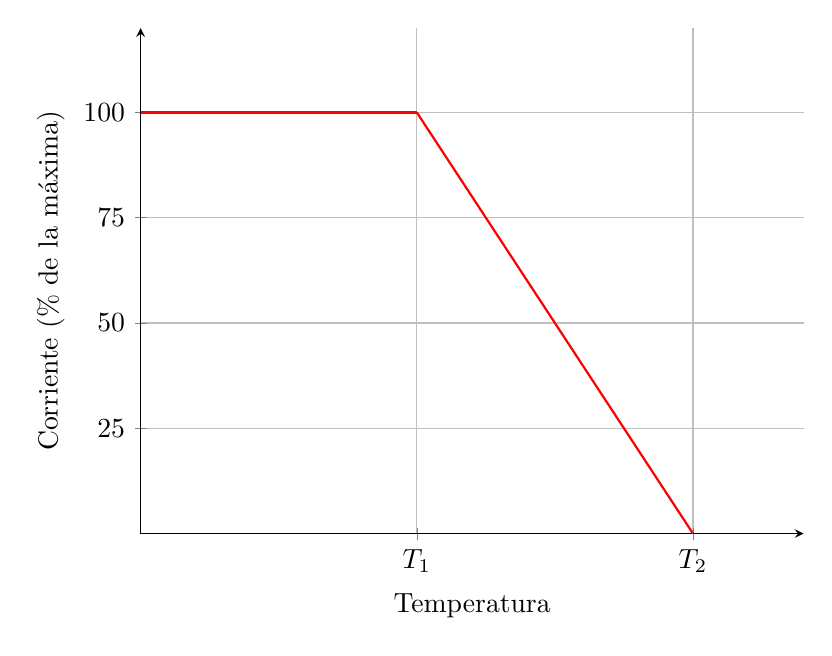
\begin{tikzpicture}
		\begin{axis}[
			axis lines=middle,
			width=10cm,
			height=8cm,
			x label style={at={(axis description cs:0.5,-0.1)},anchor=north},
			y label style={at={(axis description cs:-0.1,0.5)},rotate=90,anchor=south},
			xlabel={Temperatura},
			ylabel={Corriente (\% de la máxima)},
			xmin=0, xmax=120,
			ymin=0, ymax=120,
			xtick={50, 100},
			xticklabels={$T_1$, $T_2$},
			ytick={0, 25, 50, 75, 100},
			grid=both,
			legend pos=north west,
			legend style={font=\small},
			]
			\addplot[red, domain=0:50, samples=100, thick] {100};
			\addplot[red, domain=50:100, samples=100, thick] {200-2*x};
			
		\end{axis}
	\end{tikzpicture}
	\caption{\textit{Derating} lineal de corriente en función de la temperatura, que entra en funcionamiento a partir de $T_1$ y si se llega a $T_2$, no se entrega corriente.}
\end{figure}

\subsubsection{\texttt{PCB\_IO.c/.h}}

Los archivos \texttt{PCB\_IO.c} y su encabezado correspondiente \texttt{PCB\_IO.h} actúan como capa de abstracción del \textit{hardware}. En \texttt{PCB\_IO.h}, se definen macros para leer y controlar algunos GPIOs, así como enumeraciones y estructuras para manejar LEDs y direcciones de motores.

Las funciones principales implementadas en \texttt{PCB\_IO.c} son:

\begin{itemize}
	\item \texttt{handle\_LED}: Esta función maneja los modos de parpadeo de los LEDs basándose en el modo actual del LED y un contador de milisegundos.
	\item \texttt{handle\_direction}: Esta función lee el estado del interruptor de dirección (\texttt{DIR}) y actualiza las direcciones de los motores izquierdo y derecho en función de este estado.
	\item \texttt{enable\_inverters}: Esta función lee el estado de la cadena de \textit{shutdown} del vehículo y habilita o deshabilita los inversores en función de este estado y de una habilitación externa por \textit{software}.
\end{itemize}

\subsubsection{\texttt{CONTROL.c/.h}}

Los archivos \texttt{CONTROL.c} y su encabezado correspondiente \texttt{CONTROL.h} proporcionan funciones para el lazo de control de cada inversor. Las funciones principales implementadas en \texttt{CONTROL.c} son:

\begin{itemize}
	\item \texttt{calc\_current\_reference}: Esta función calcula las consignas de corriente $d - q$ de la misma manera que en las simulaciones de control. Se implementan las trayectorias utilizando las ecuaciones analíticas de las mismas.
	\item \texttt{calc\_current\_loop}: Esta función ejecuta los lazos de corriente para los ejes $d$ y $q$.
	\item \texttt{saturate\_voltage}: Esta función satura la salida de los lazos de corriente para no exceder el voltaje máximo sintetizable.
	\item \texttt{calc\_duties}: Esta función calcula la transformada inversa de Park y los ciclos de trabajo utilizando SVPWM.
\end{itemize}

Cabe destacar que este archivo hace uso de la librería PERGAMON del CITCEA-UPC, relacionando las diferentes partes del código con la simulación realizada anteriormente. Los bloques usados en la simulación contienen el mismo código que está escrito en estas librerías, agilizando mucho la integración.

\subsubsection{\texttt{PWM.c/.h}}

Los archivos \texttt{PWM.c} y su encabezado correspondiente \texttt{PWM.h} proporcionan funciones para controlar la salida PWM. Hace de capa de abstracción de los \textit{timers}, ya que contiene funciones para habilitar y deshabilitar la salida PWM y para actualizar los ciclos de trabajo.


\subsubsection{\texttt{CAN\_e-Tech.c/.h}}

Los archivos \texttt{CAN\_e-Tech.c} y su encabezado correspondiente \texttt{CAN\_e-Tech.h} proporcionan funciones para manejar la comunicación CAN con el vehículo. Las funciones principales implementadas en \texttt{CAN\_e-Tech.c} son:

\begin{itemize}
	\item \texttt{handle\_CAN}: Esta función implementa la lógica para manejar mensajes CAN recibidos.
	\item \texttt{send\_CAN\_message}: Esta función prepara y envía un mensaje CAN utilizando información de \texttt{CAN1db.h}, que recoge la estructura de todos los mensajes del bus de CAN al cual estará conectado el inversor.
\end{itemize}

\subsection{Implementación del \textit{firmware}}

\subsubsection{Configuración del MCU}
Como ya se ha mencionado, se usará CubeMX para configurar los periféricos del microcontrolador. Las configuraciones más importantes se detallan a continuación.

\textbf{Reloj}

Es crucial configurar adecuadamente el reloj del microcontrolador para que este pueda medir tiempos de forma precisa. En este caso se usa un cristal de cuarzo externo de 20 MHz como referencia, y se trata internamente para lograr llegar a los 216 MHz máximos del microcontrolador.

\begin{figure}[H]
	\centering
	\includegraphics[width=0.7\linewidth]{fig/cubeMXclock}
	\caption{Configuración del reloj del sistema.}
\end{figure}


\textbf{GPIOs}

Se configuran como entradas / salidas los pines individuales de cada señal, asignándoles un nombre descriptivo acorde con el esquemático de la placa de control.

\begin{figure}[H]
	\centering
	\includegraphics[width=0.8\linewidth]{fig/cubeMXGPIOs}
	\caption{Configuración de GPIOs.}
\end{figure}

\textbf{ADCs}

En el control del convertidor es importante que las lecturas analógicas sean capturadas en una ventana de tiempo específica, generalmente sincrónica con la frecuencia de conmutación. En este caso, se han configurado dos ADCs (uno por cada inversor) con la adquisición disparada con el desbordamiento de su respectivo \textit{timer}. Se capturan cuatro canales por inversor, los tres primeros se corresponden con las corrientes de fase, y el último, con la tensión del bus DC. Un punto importante es que el ADC usa un \textit{stream} de DMA para volcar la información directamente en la memoria en un \textit{buffer}, aliviando algo de carga al MCU. Cuando se necesitan las medidas, se leen directamente del \textit{buffer}, que estará preparado con las últimas medidas tomadas.

\begin{figure}[H]
	\centering
	\includegraphics[width=0.7\linewidth]{fig/cubeMXADC}
	\caption{Configuración del ADC 2 por DMA, correspondiente al inversor izquierdo.}
\end{figure}

Dado que la temperatura tiene una dinámica muy lenta, no es necesario tomar medidas a la frecuencia de control. Por ello se enrutan las medidas de temperatura a un ADC separado y se leen de forma más lenta.

\begin{figure}[H]
	\centering
	\includegraphics[width=0.7\linewidth]{fig/cubeMXADC3}
	\caption{Configuración del ADC para la adquisición de temperaturas.}
\end{figure}

\textbf{\textit{Timers}}

Los periféricos más importantes son los \textit{timers}, ya que el control es síncrono. Por ello se han configurado dos \textit{timers}, uno para cada inversor. Las salidas PWM se controlan directamente con los \textit{timers}, que a su vez, disparan la lectura de los ADCs. Los \textit{timers} 1 y 8, encargados de los lazos de control izquierdo y derecho respectivamente, tienen una peculiaridad: pueden generar tres canales duplicados, donde tres de ellos mantienen su polaridad positiva y los otros tres son réplicas con polaridad invertida de los primeros. Además, estos periféricos facilitan la integración de características propias de una salida complementaria como la definición del tiempo muerto. La gestión se realiza de forma automática por parte del mismo \textit{timer}.

Se ajustan las constantes correspondientes al periodo de conmutación y al tiempo muerto utilizando \texttt{\#define TS} y \texttt{\#define DT}, de manera que se puede modificar la frecuencia de conmutación muy fácilmente. Se configuran los \textit{timers} en modo \textit{up and down}, simulando una señal portadora triangular, de la misma manera que está configurada la conmutación en la simulación de PLECS. Si contara solamente hacia arriba o hacia abajo, la portadora sería una señal diente de sierra.

\begin{figure}[H]
	\centering
	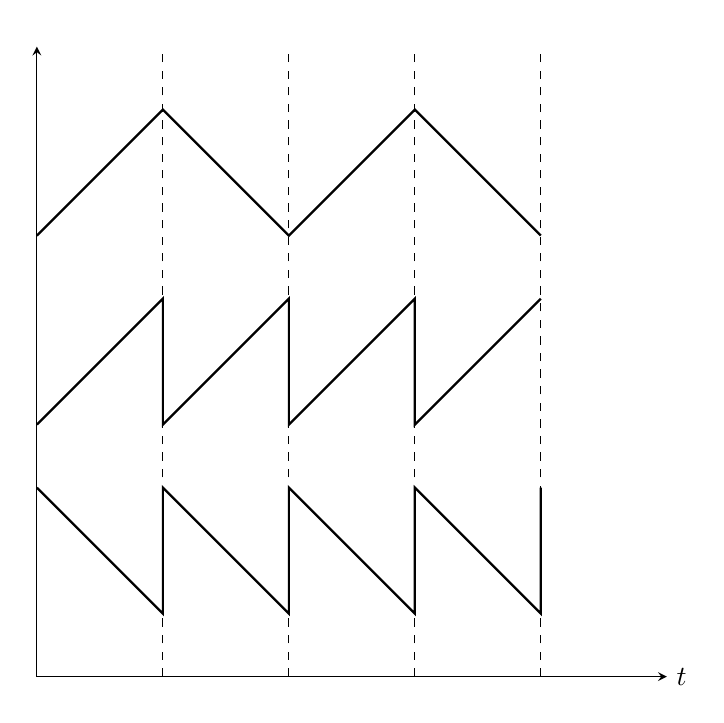
\begin{tikzpicture}[scale=0.8]
		% Ejes y etiquetas
		\draw[-stealth] (0,-7) -- (10,-7) node[right] {$t$};
		\draw[-stealth] (0,-7) -- (0,3) node[above]{$ $};
		
		% Señales
		\draw[dashed] (2,-7) -- (2,3);
		\draw[dashed] (4,-7) -- (4,3);
		\draw[dashed] (6,-7) -- (6,3);
		\draw[dashed] (8,-7) -- (8,3);
		
		% Señal triangular
		\draw[thick] (0,0) -- (2,2) -- (4,0) -- (6,2) -- (8,0);
		
		% Señal de sierra
		\draw[thick] (0,-3) -- (2,-1) -- (2,-3) -- (4,-1) -- (4,-3) -- (6,-1) -- (6,-3) -- (8,-1);
		
		% Señal de sierra invertida
		\draw[thick] (0,-4) -- (2,-6) -- (2,-4) -- (4,-6) -- (4,-4) -- (6,-6) -- (6,-4) -- (8,-6) -- (8,-4);
		
	\end{tikzpicture}
	\caption{Comparación de las señales portadoras equivalentes. De arriba a abajo, triangular, diente de sierra y diente de sierra invertida.}
\end{figure}

\begin{figure}[H]
	\centering
	\includegraphics[width=0.7\linewidth]{fig/cubeMXtimer1}
	\caption{Configuración del \textit{timer} 1, correspondiente al inversor izquierdo.}
\end{figure}

\textbf{CAN}

Para poder comunicarse externamente se usa el protocolo CAN. Por suerte, la configuración es muy sencilla. Se deben ajustar los parámetros para que la frecuencia de transmisión de datos (\textit{baud rate}) sea de 500 kB/s exactamente, ya que el resto de ECUs en el monoplaza tienen el periférico configurado a esta frecuencia.

\begin{figure}[H]
	\centering
	\includegraphics[width=0.7\linewidth]{fig/cubeMXCAN}
	\caption{Configuración del periférico CAN.}
\end{figure}

\subsubsection{Manejo de interrupciones}

En un convertidor se debe tener control absoluto sobre \textit{cuándo} se ejecuta \textit{qué}. Esto quiere decir que el lazo de control debe seguir un orden de ejecución perfectamente definido. El orden se basa en las simulaciones realizadas en PLECS, que como ya se explicó, tienen una relación muy estrecha con la implementación del \textit{firmware}. Estudiando \cite{Buso2006} y \cite{carlos2023}, se decide seguir el siguiente orden en las interrupciones de control:
\begin{enumerate}
	\item Se inicia la conversión de las lecturas analógicas de las corrientes y la tensión.
	\item Cuando acaba la conversión, se evalúan los valores obtenidos para hacer saltar errores si estuvieran fuera de los límites. Se establece la tensión máxima sintetizable en el periodo.
	\item Se calcula la consigna de corriente.
	\item Se ejecutan los lazos de corriente.
	\item Se satura la tensión de salida.
	\item Se calculan los ciclos de trabajo y se actualiza el registro del \textit{timer} de la salida PWM.
\end{enumerate}

La conversión del ADC se inicia periódicamente con el \textit{timer} correspondiente. El resto de tareas se implementan en una función vacía. Lo que se desea lograr se muestra en la figura \ref{carrier}.

\begin{figure}[H]
	\centering
	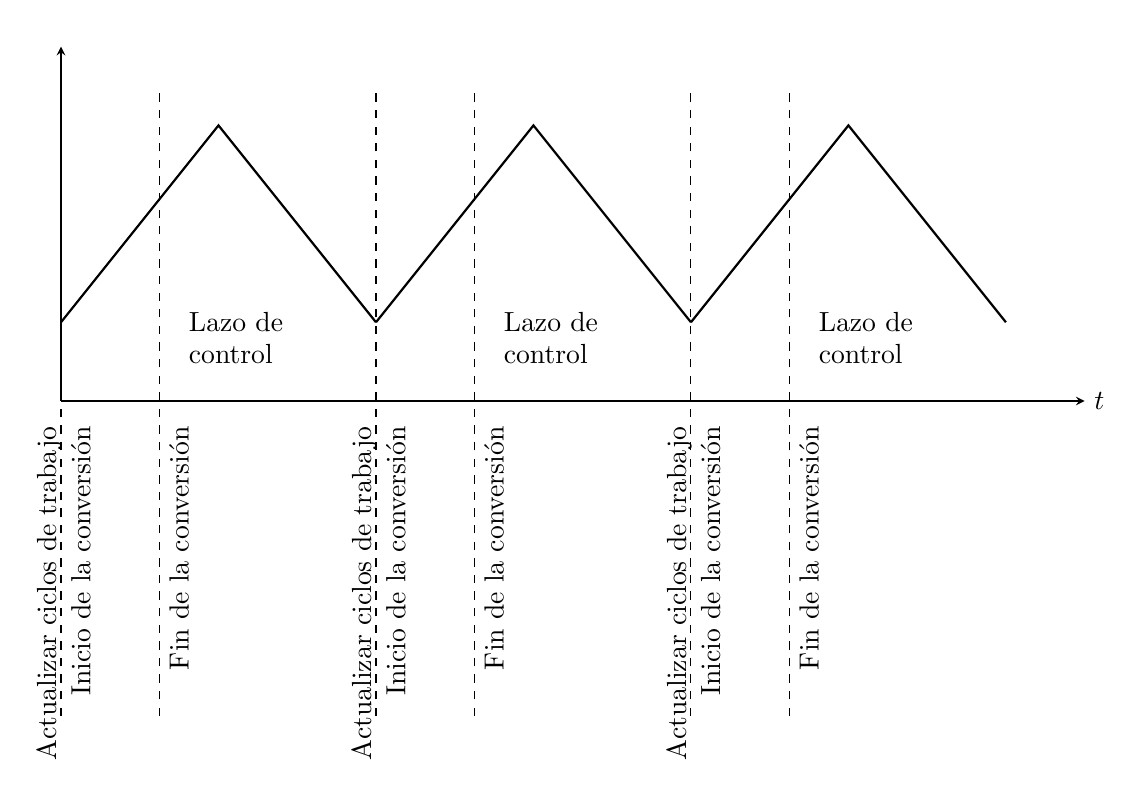
\begin{tikzpicture}[scale=1]
		% Parámetros
		\def\n{2} % Número de periodos
		
		% Ejes y etiquetas
		\draw[-stealth] (0,-1) -- (4*\n+5,-1) node[right] {$t$};
		\draw[-stealth] (0,-1) -- (0,3.5) node[above]{$ $};
		
		% Líneas verticales y etiquetas
		\foreach \i in {0,...,\n} {
			\draw[dashed] (4*\i,-5) -- (4*\i,3);
			\node at (4*\i-0.15,-1.2) [anchor=east, rotate=90] {Actualizar ciclos de trabajo};
			\node at (4*\i+0.25,-1.2) [anchor=east, rotate=90] {Inicio de la conversión};
			\draw[dashed] (4*\i+1.25,-5) -- (4*\i+1.25,3);
			\node at (4*\i+1.5,-1.2) [anchor=east, rotate=90] {Fin de la conversión};
            \node at (4*\i+1.5,0) [anchor=west] {Lazo de};
			\node at (4*\i+1.5,-0.4) [anchor=west] {control};
		}
		
		% Señal triangular
		\foreach \i in {0,...,\n} {
			\draw[thick] (4*\i,0) -- (4*\i+2,2.5) -- (4*\i+4,0);
		}
		
	\end{tikzpicture}
	\caption{Señal portadora (registro CNT del \textit{timer}) durante 3 periodos de conmutación y los eventos asociados.}
	\label{carrier}
\end{figure}


La implementación de código se maneja con la interrupción generada al final de las conversiones analógicas.

\begin{adjustbox}{max width=3\textwidth}
\begin{lstlisting}[language=C, breaklines=true, frame=single]

/**
* @brief Function to be executed every TS.
*
* This function is called by the ADC2 DMA handler every TS (ADC is triggered with TIM1).
*/
void tasks_critical_left(void){
	start_ticks = SysTick->VAL;
	
	// ADC
	get_currents_voltage(rawADC_left, &inverter_left.analog, &inverter_left.feedback, &inverter_left.errors, inverter_right.encoder.sinTheta_e, inverter_left.encoder.cosTheta_e);
	inverter_left.vsMax = 0.9F * inverter_left.analog.vDC * ISQ3; // Calculate max Vs voltage with a safety margin
	
	// FOC
	calc_current_reference(inverter_left.motor, &inverter_left.reference);
	
	// PIs and duty calc
	calc_current_loop(&inverter_left);
	saturate_voltage(&inverter_left);
	calc_duties(inverter_left.vd, inverter_left.vq, inverter_left.analog.vDC, inverter_left.encoder.sinTheta_e, inverter_left.encoder.cosTheta_e, &inverter_left.duties);
	
	update_PWM(inverter_left.htim, inverter_left.duties);
	
	
	elapsed_ticks = start_ticks - SysTick->VAL;
	
}	
\end{lstlisting}
\end{adjustbox}

Esta función vacía se llama dentro de la interrupción del ADC, que salta cuando el DMA llena el \textit{buffer} de datos, indicando que se ha completado la conversión.


\begin{adjustbox}{max width=\textwidth}
\begin{lstlisting}[language=C, breaklines=true, frame=single]
/**
* @brief This function handles DMA2 stream2 global interrupt.
*/
void DMA2_Stream2_IRQHandler(void)
{
	/* USER CODE BEGIN DMA2_Stream2_IRQn 0 */
	
	/* USER CODE END DMA2_Stream2_IRQn 0 */
	HAL_DMA_IRQHandler(&hdma_adc2);
	/* USER CODE BEGIN DMA2_Stream2_IRQn 1 */
	tasks_critical_left();
	
	/* USER CODE END DMA2_Stream2_IRQn 1 */
}
\end{lstlisting}
\end{adjustbox}

\subsubsection{Lazo de control}

El algoritmo \texttt{calc\_current\_reference} calcula las referencias de corriente a partir de la consigna de par. Este algoritmo se encarga de calcular la trayectoria MTPA y limita la consigna de corriente a \texttt{isMaxRef}, que se satura usando el \textit{derating} implementado anteriormente. La trayectoria MTPV no está implementada para optimizar el tiempo de cálculo debido a las características esperadas de los motores que se controlarán. Finalmente, se convierten las coordenadas polares de las referencias de corriente (\texttt{isRef} y \texttt{gammaRef}) a coordenadas cartesianas  (\texttt{idRef} e \texttt{iqRef}).

También se deja un espacio para la implementación de debilitamiento de campo. Para implementarlo, se debe añadir el lazo de tensión para modificar \texttt{gammaRef} y la trayectoria VLE. Además se debería implementar una selección de trayectorias adecuada que permita trabajar en todos los puntos de operación.

Para conocer el tiempo de ejecución del algoritmo, y de cualquier parte del código, se puede utilizar el \textit{timer} interno \texttt{SysTick} para contar los ciclos de reloj entre dos puntos del código. Se observó que es necesario activar la optimización de velocidad en las opciones del compilador para que los cálculos entren dentro del tiempo de conmutación de 25 \unit{\micro\second}. Se estaban obteniendo valores de unos 3000 ciclos antes de activar la optimización, y de 1800 después de activarla. Aún así, sería buena idea dejar más margen mediante un estudio de optimización del propio código, evitando cálculos innecesarios o proponiendo nuevas maneras de calcular funciones trigonométricas, que son las que más tiempo llevan.

\begin{figure}[H]
	\centering
	\includegraphics[width=0.7\linewidth]{fig/compilerOptimize}
	\caption{Optimización de velocidad en el compilador.}
\end{figure}


